\documentclass{aa}
\usepackage{amsmath}
\usepackage{hyperref}
\usepackage{xcolor}


\title{Gaps in stellar streams as a result of globular cluster fly-bys}

\subtitle{The case of Palomar~5}

\author{Salvatore Ferrone
       \inst{1,2,3}
         \and
       Marco Montuori\inst{3}
       \and
       Paola Di Matteo\inst{1}
       \and
       Alessandra Mastrobuono-Battisti \inst{4}
       \and 
       Rodrigo Ibata \inst{5}
       \and 
       Paolo Bianchini \inst{5}
       \and
       Sergey Khoperskov \inst{6}
       \and
       Nicolas Leclerc \inst{7}
       \and 
       Clement Hottier \inst{7}
       \and 
       Eliot Stein  \inst{8}
       \and
       David Valls-Gabaud \inst{9}
       \and
       Owain N. Snaith \inst{10}
       \and
       Misha Haywood \inst{1}
       }

\institute{
    LIRA, Observatoire de Paris, Université PSL, Sorbonne Université, Université Paris Cité, CY Cergy Paris Université, CNRS,  92190 Meudon, France\\
  \email{salvatore.ferrone@obspm.fr}
  \and
    Department of Physics, University  of Rome ``La Sapienza'' Piazzale Aldo Moro 5, 00185 Rome, Italy.
  \and 
    Institute for Complex Systems CNR, Piazzale Aldo Moro 2, 00185 Rome, Italy
  \and
    Dipartimento di Fisica e Astronomia. ``Galileo Gallilei'' Università di Padova, Vicolo dell'Osservatorio 3 Padova 35122, Italy.
  \and
    Universit\'e de Strasbourg, CNRS, Observatoire astronomique de Strasbourg, UMR 7550, F-67000 Strasbourg, France
  \and
    Leibniz-Institut für Astrophysik Potsdam (AIP), An der Sternwarte 16, 14482 Potsdam, Germany
  \and
    UNIDIA, Observatoire de Paris, Université PSL, CNRS, 92190 Meudon, France
  \and
    DTIS, ONERA, Université Paris Saclay, 91123 Palaiseau, France 
  \and
    LUX, CNRS UMR 8252, Observatoire de Paris, PSL, 61 Avenue de l'Observatoire, 75014 Paris, France
  \and
    Department of Physics and Astronomy, University of Exeter, Stocker Rd, Exeter EX4 4QL, United Kingdom
  }
      
  \date{Accepted 26 May 2025}

  \begin{document}
    \abstract
      {Thin stellar streams, such as those resulting from the tidal disruption of globular clusters, have long been known and used as probes of the gravitational potential of our Galaxy, both its visible and dark contents. The literature commonly interprets the presence of under-density regions, or gaps, along these streams as being due to the close passage of dark matter sub-halos. }
      {In this work, we investigate the perturbations induced on streams by the passage of dense stellar systems, such as globular clusters themselves, to test the possibility that they may cause the formation of gaps as well. In particular, we focus on the study of the stream generated by a cluster with characteristics (mass, size, and orbit) similar to the current characteristics of Palomar~5, a well-known globular cluster in the Galactic halo, which has particularly long tidal tails.  }
      {For this purpose, we used a particle-test code to simulate the formation and evolution of the stream when subjected to the Galaxy's gravitational field plus its whole system of globular clusters.}
      {Our study shows that such a stream can be strongly perturbed by the close passage of other clusters, in particular of NGC~2808, NGC~7078, and NGC~104, and that these perturbations induce the formation of gaps in the tails.}
      {These results show that globular clusters can induce gaps in cold streams--just as it has been demonstrated in the literature for that other baryonic components, such as giant molecular clouds and the galactic bar, may as well. Therefore, a future work that attempts to infer the dark matter sub-halo distribution from stellar stream gaps must include the contributions from globular clusters.}


    \maketitle

  \section{Gallery of gaps} \label{sec:gallery_of_gaps}
    Figures~\ref{fig:gallery0}-\ref{fig:gallery11} include all of the realizations of the \texttt{full} simulations of Palomar~5 in tail coordinates. A red arrow aids the reader in identifying the gap, accompanied by the responsible globular cluster. For the gaps that are not easily visible, we show the 1D profiles showing the significant under-densities compared to the \texttt{reference} simulations. For instance, the second and last panels of Fig.~\ref{fig:gallery0}. However, marginalizing the 2D distribution to 1D can erase the signal of oblique gaps. Thus, not all gaps in the 2D space are visible in the density profiles. For example, in \texttt{Sampling 000}, the gaps from NGC~2808 and NGC~5634 are not flagged as present in the marginalized density profile.

    \begin{figure*}
      \centering
      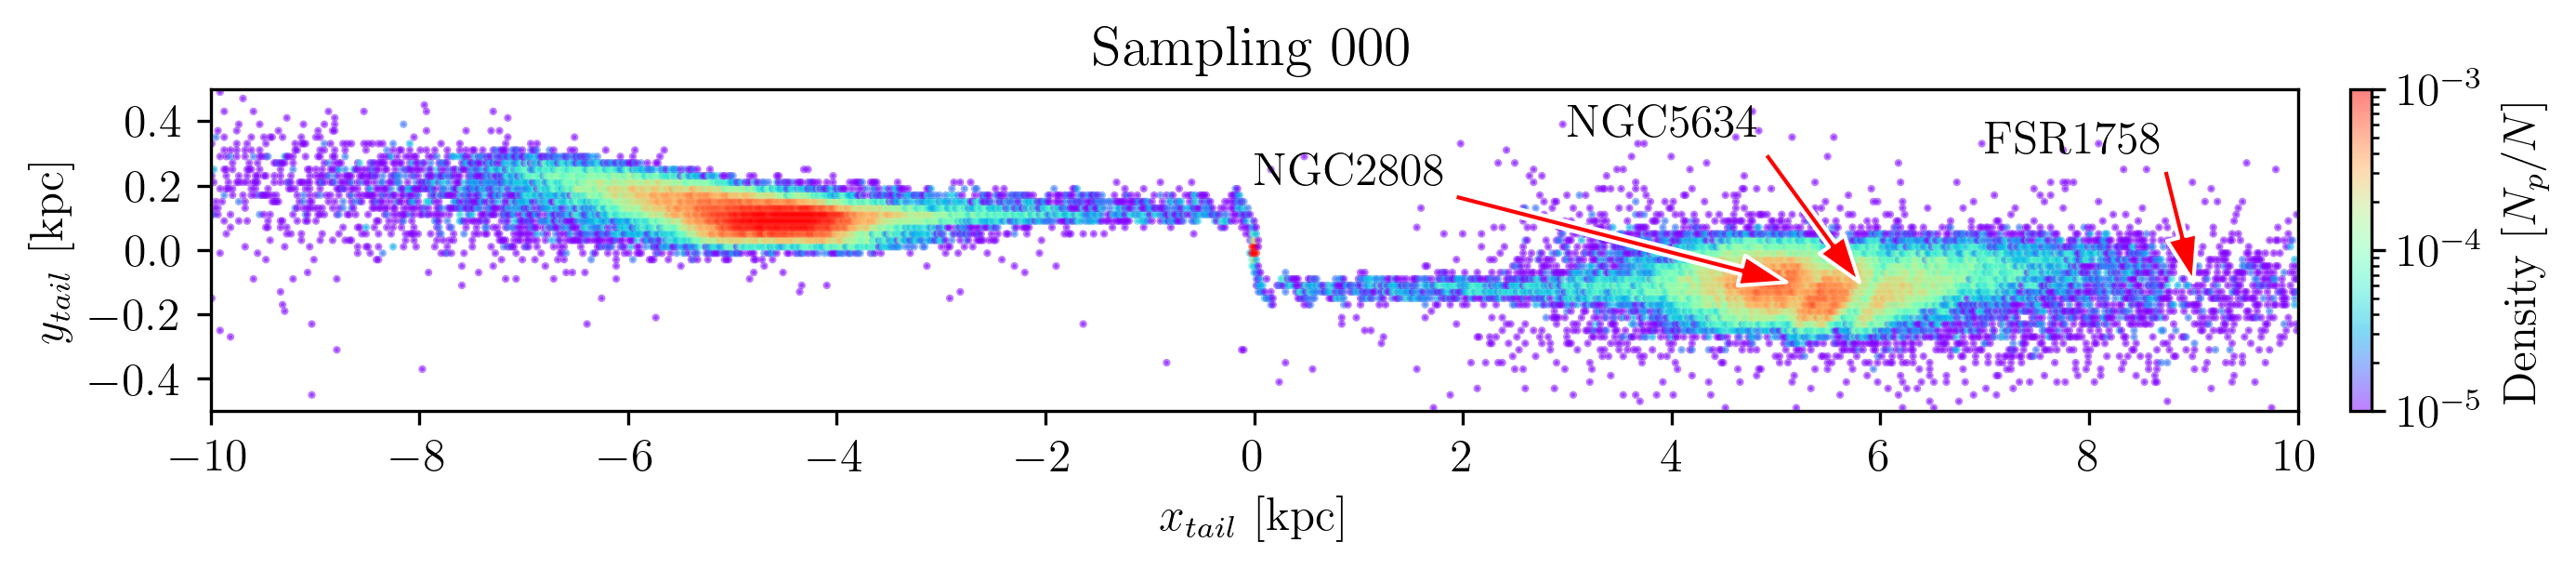
\includegraphics[width=\linewidth]{gallery_of_gaps_monte-carlo-000.png}
      
\includegraphics[width=\linewidth]{tau-profile-monte-carlo-000.png}
      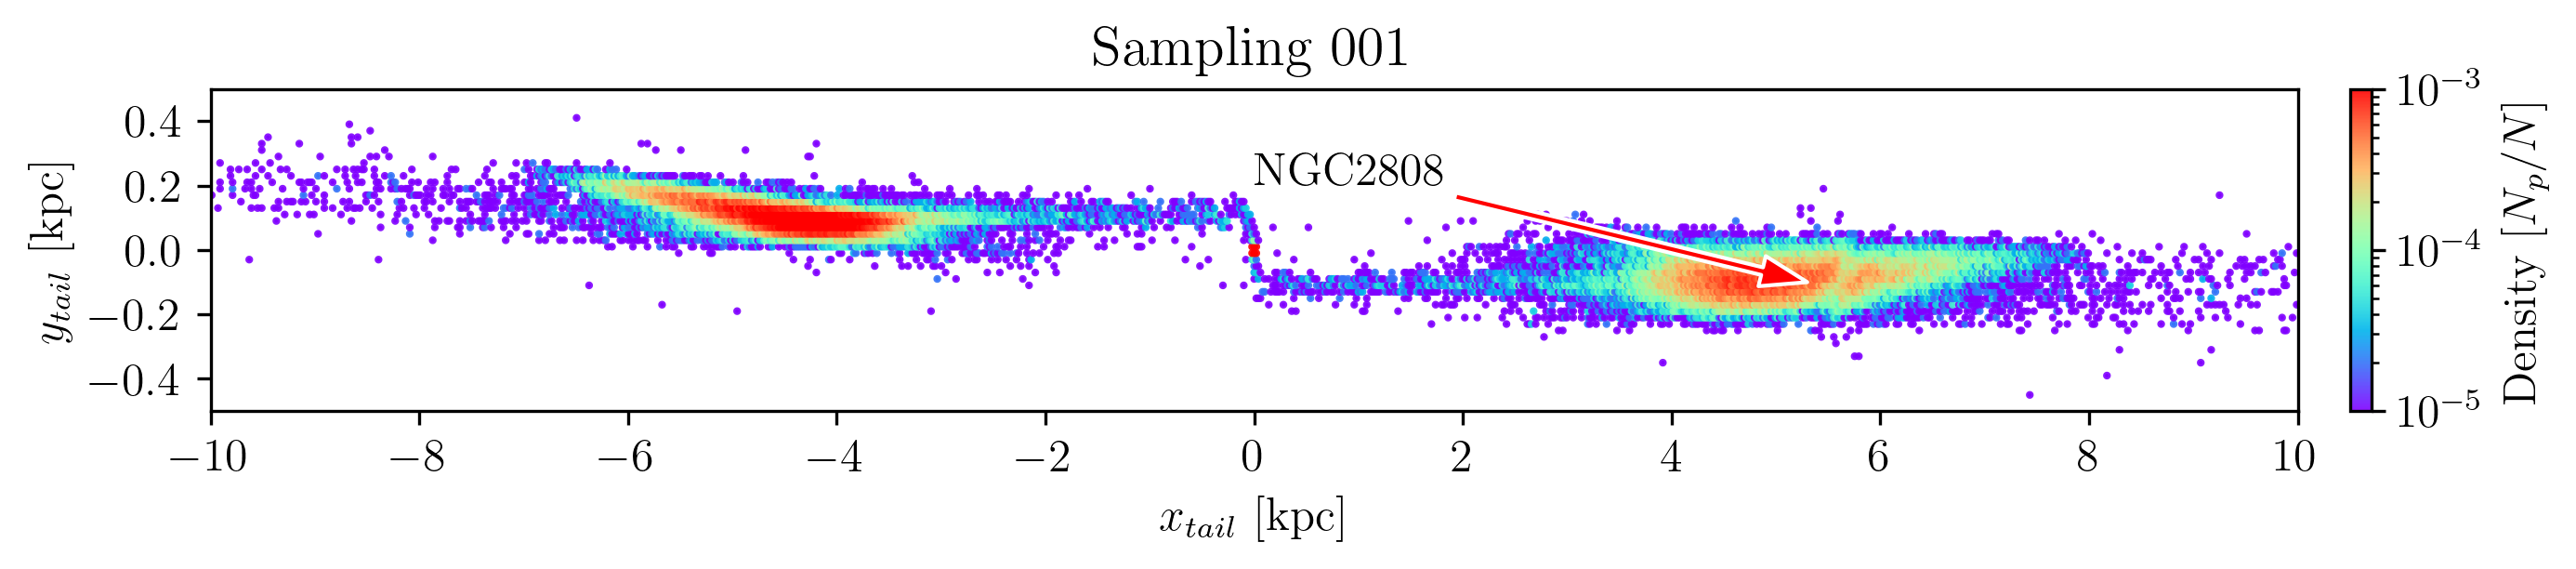
\includegraphics[width=\linewidth]{gallery_of_gaps_monte-carlo-001.png}
      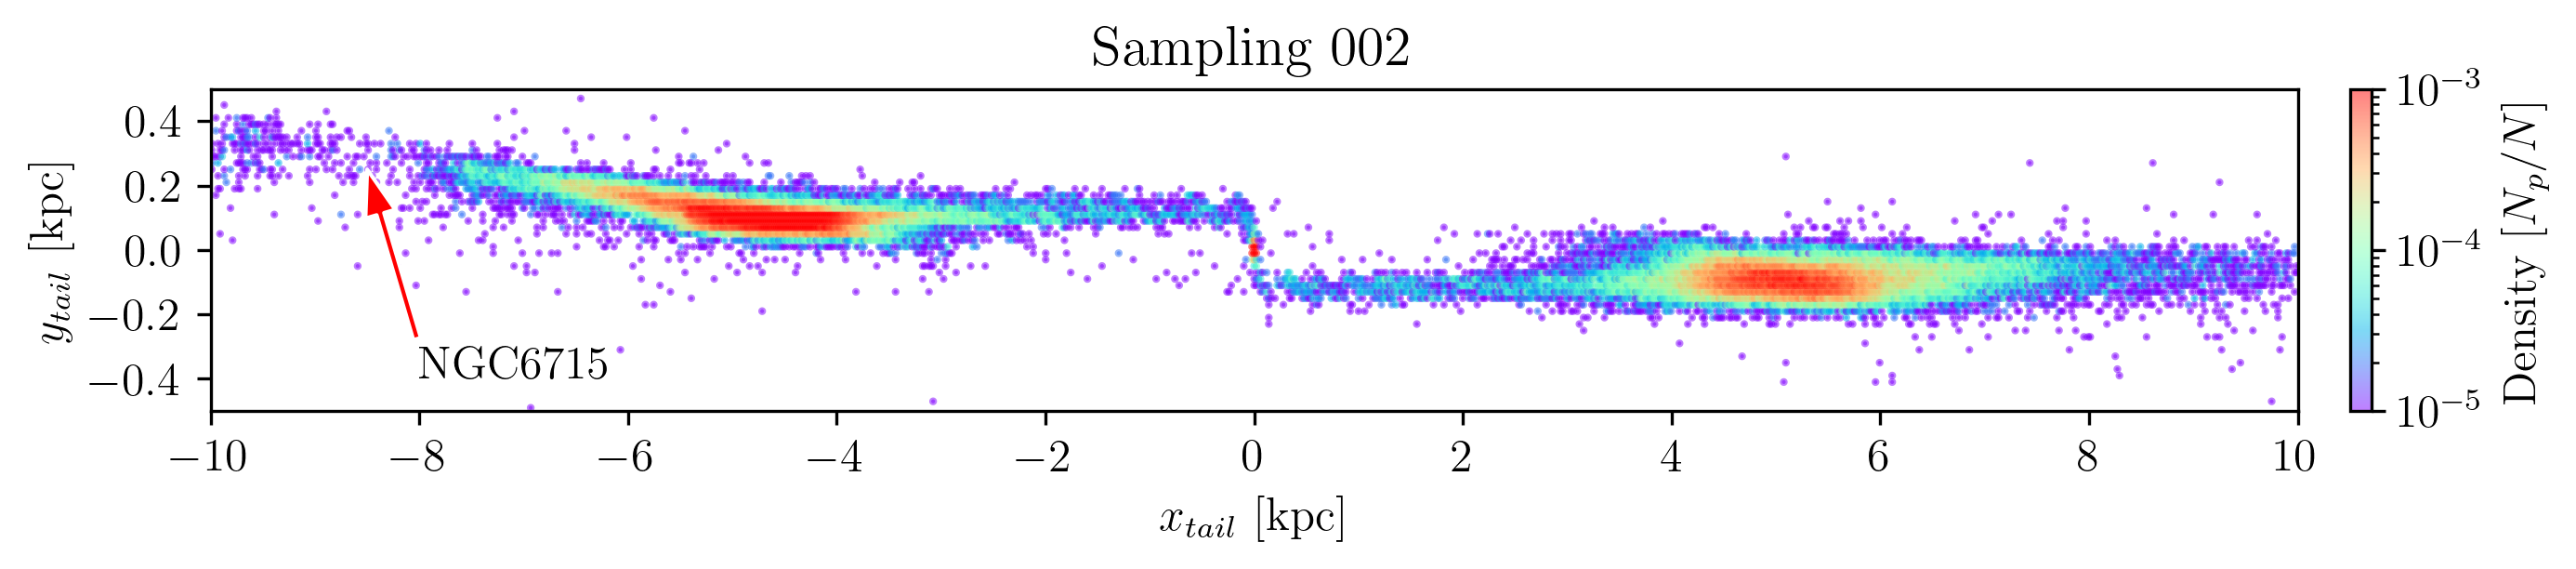
\includegraphics[width=\linewidth]{gallery_of_gaps_monte-carlo-002.png}
      
\includegraphics[width=\linewidth]{tau-profile-monte-carlo-002.png}
      \caption{First gap gallery. We present 50 Monte Carlo realizations of the Palomar~5 stream from our simulations. Gaps are labeled with arrows, along with the globular cluster responsible for each perturbation. For gaps identified via a 1D density profile, the profile is shown following the corresponding 2D density map. Gap candidates are locations where the difference between the vanilla (reference) simulation and the full simulation case exceeds the noise level. }
      \label{fig:gallery0}
      \end{figure*}

    \begin{figure*}
      \centering
      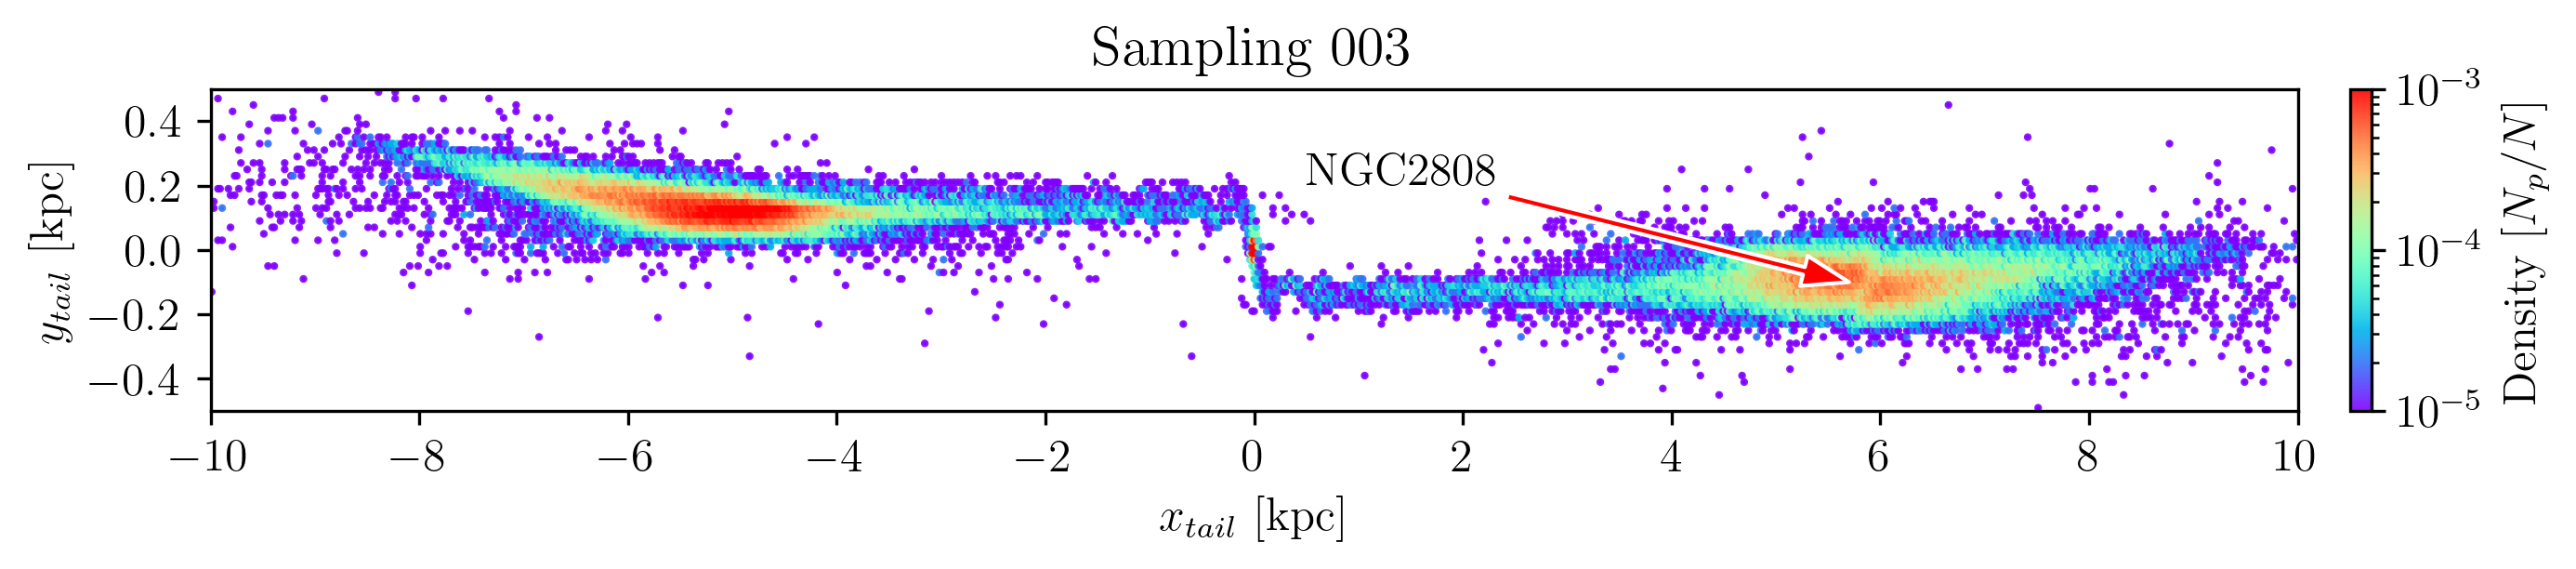
\includegraphics[width=\linewidth]{gallery_of_gaps_monte-carlo-003.png}      
      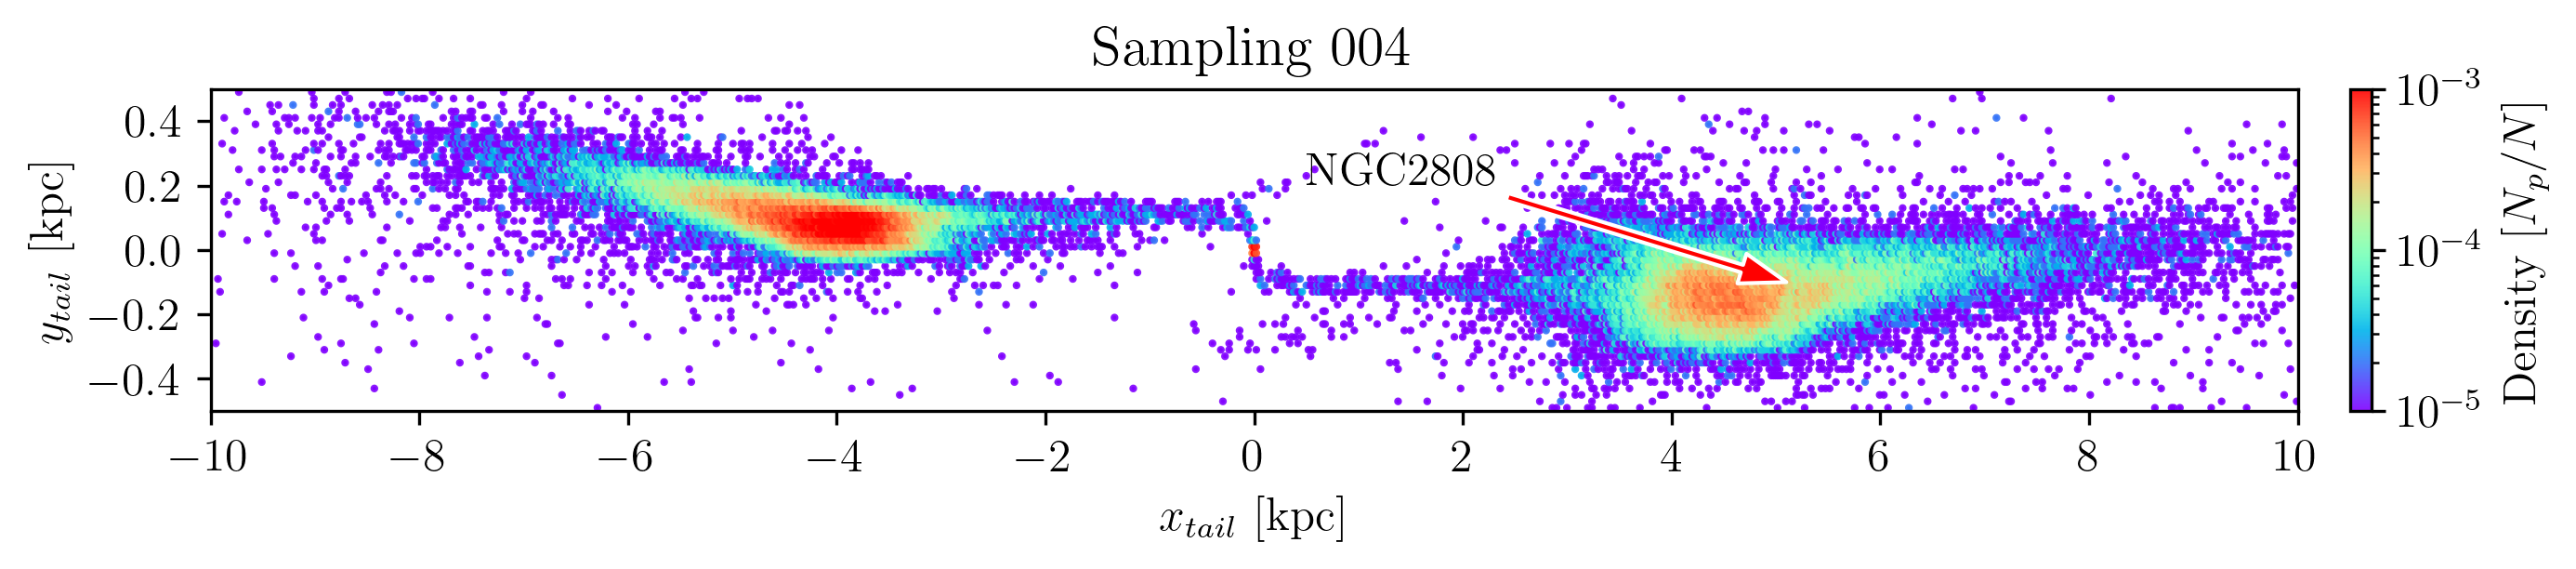
\includegraphics[width=\linewidth]{gallery_of_gaps_monte-carlo-004.png}
      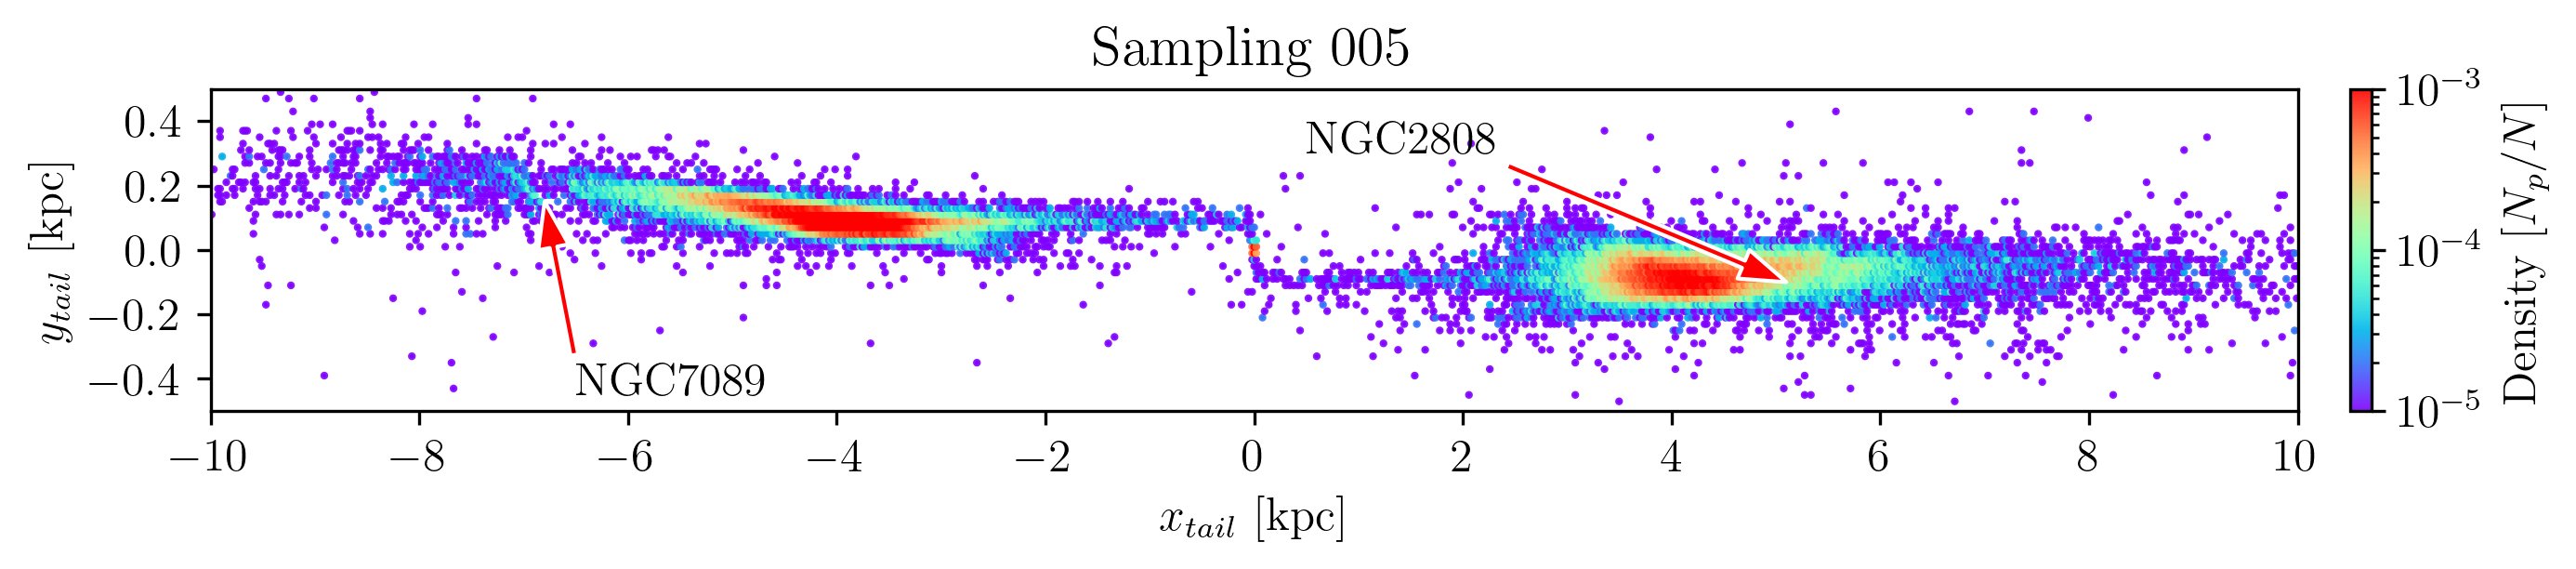
\includegraphics[width=\linewidth]{gallery_of_gaps_monte-carlo-005.png}
      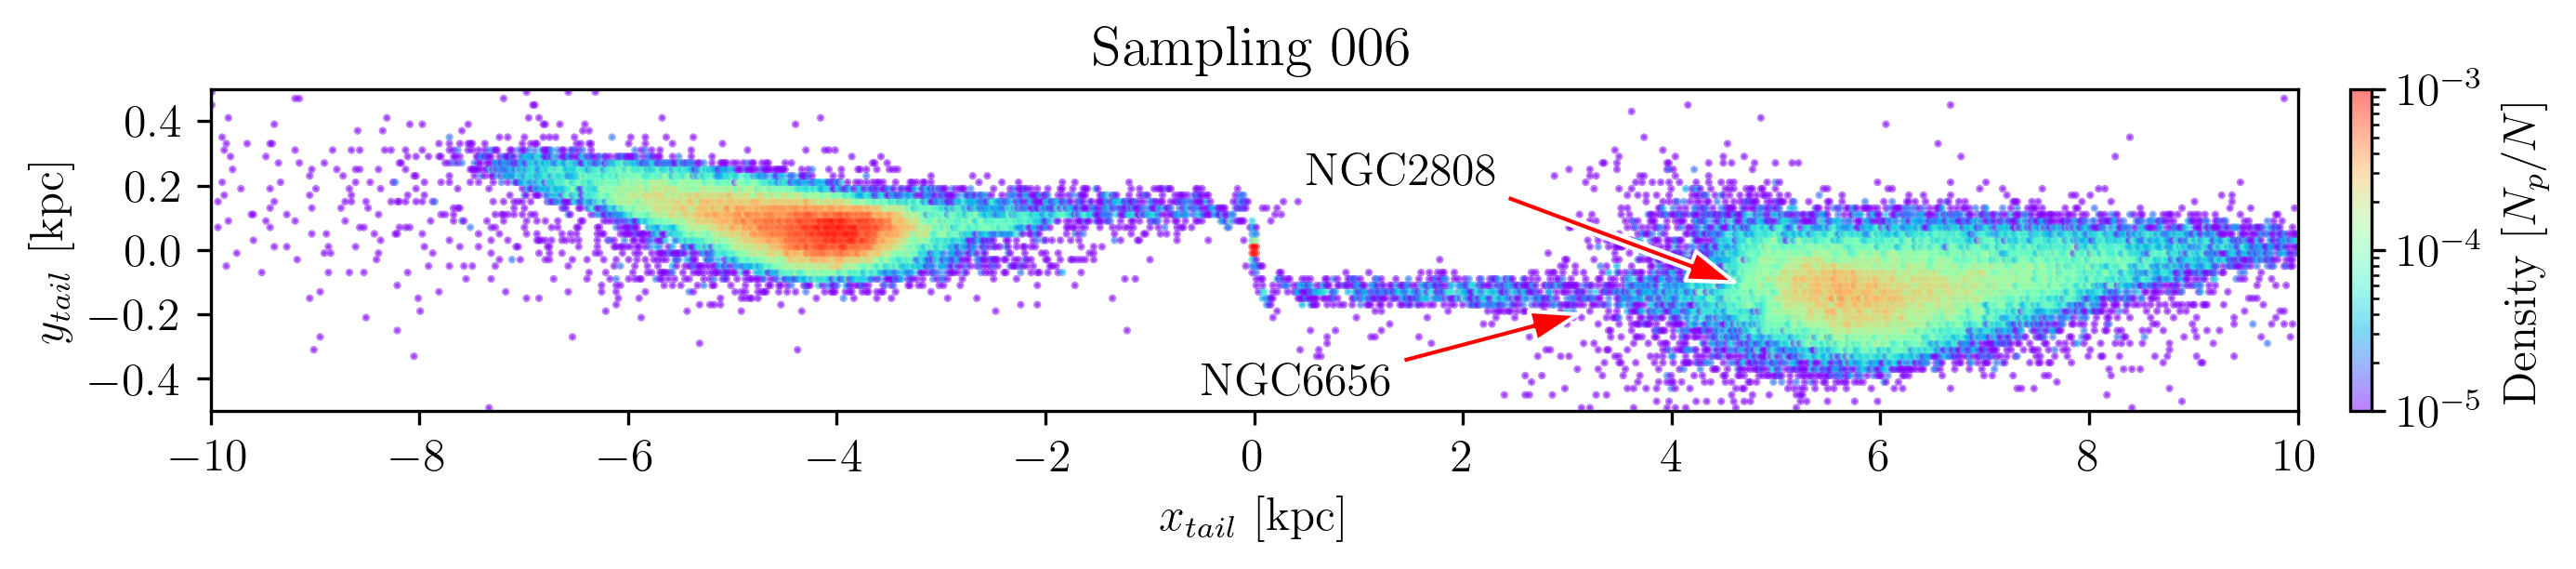
\includegraphics[width=\linewidth]{gallery_of_gaps_monte-carlo-006.png}
      
\includegraphics[width=\linewidth]{tau-profile-monte-carlo-006.png}
      \caption{Second gap gallery}
      \label{fig:gallery1}
      \end{figure*}

    \begin{figure*}
      \centering
      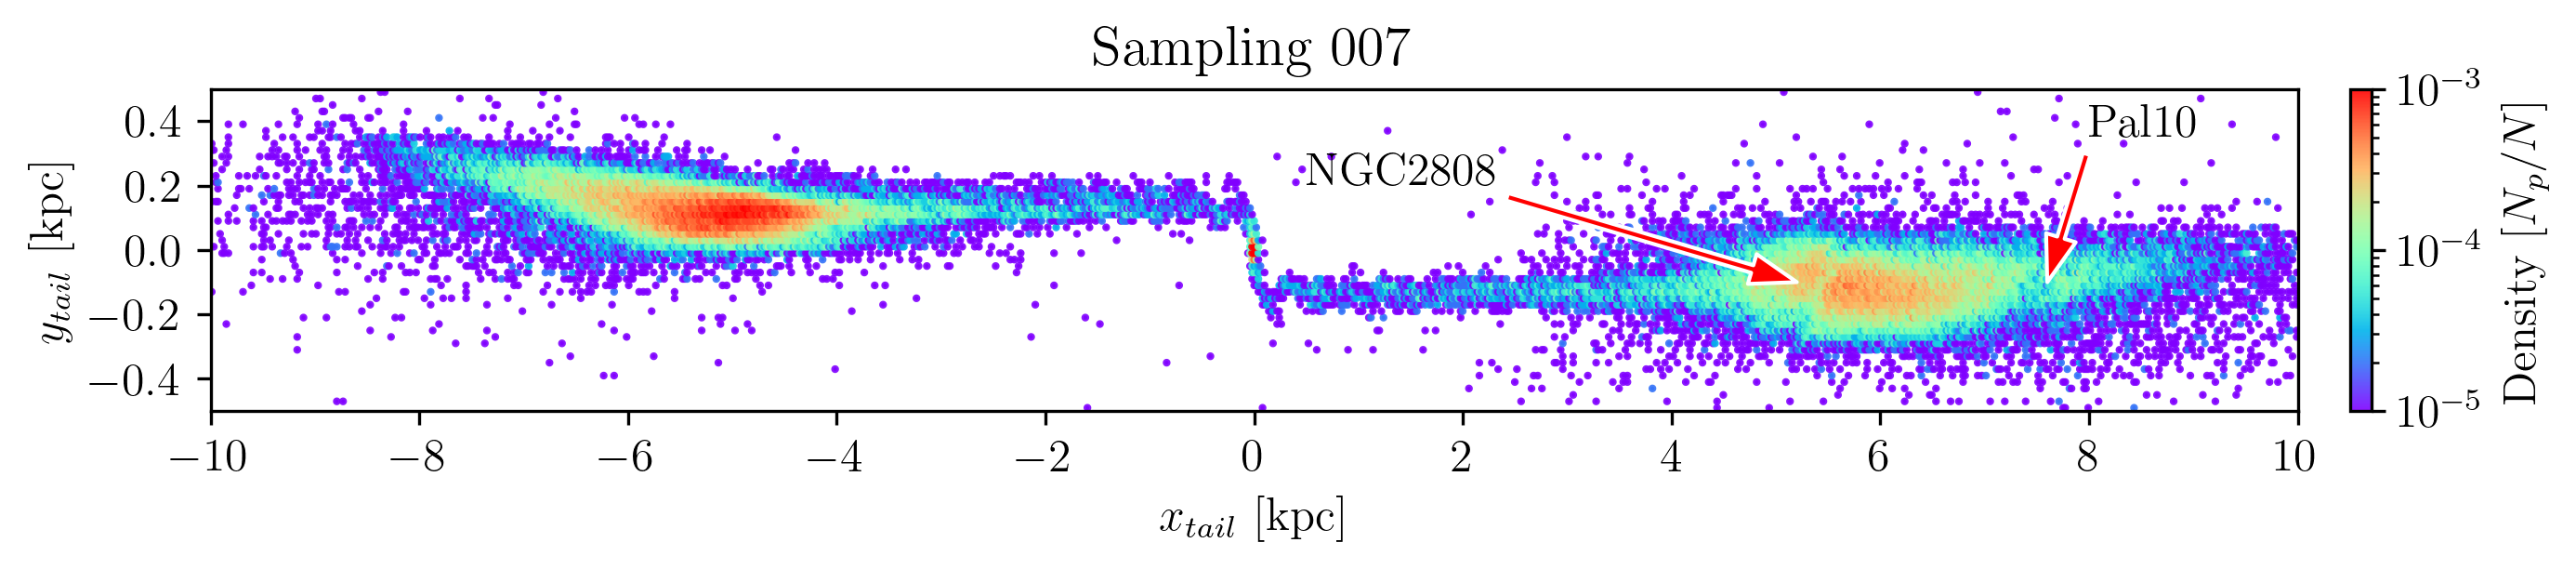
\includegraphics[width=\linewidth]{gallery_of_gaps_monte-carlo-007.png}
      
\includegraphics[width=\linewidth]{gallery_of_gaps_monte-carlo-008.png}
      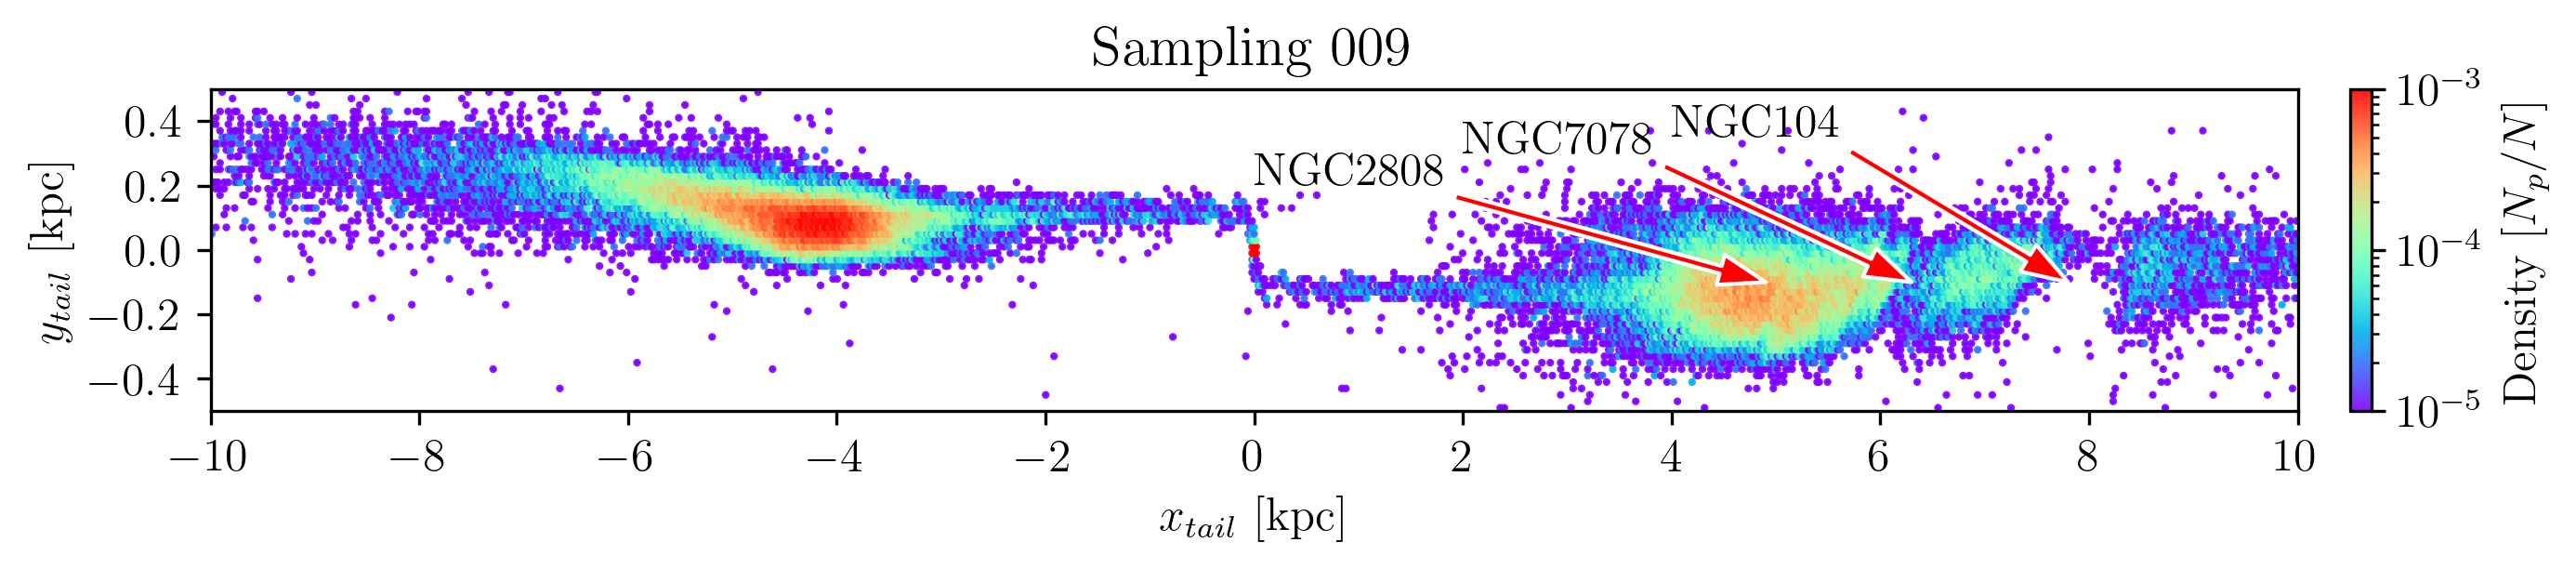
\includegraphics[width=\linewidth]{gallery_of_gaps_monte-carlo-009.png}      
      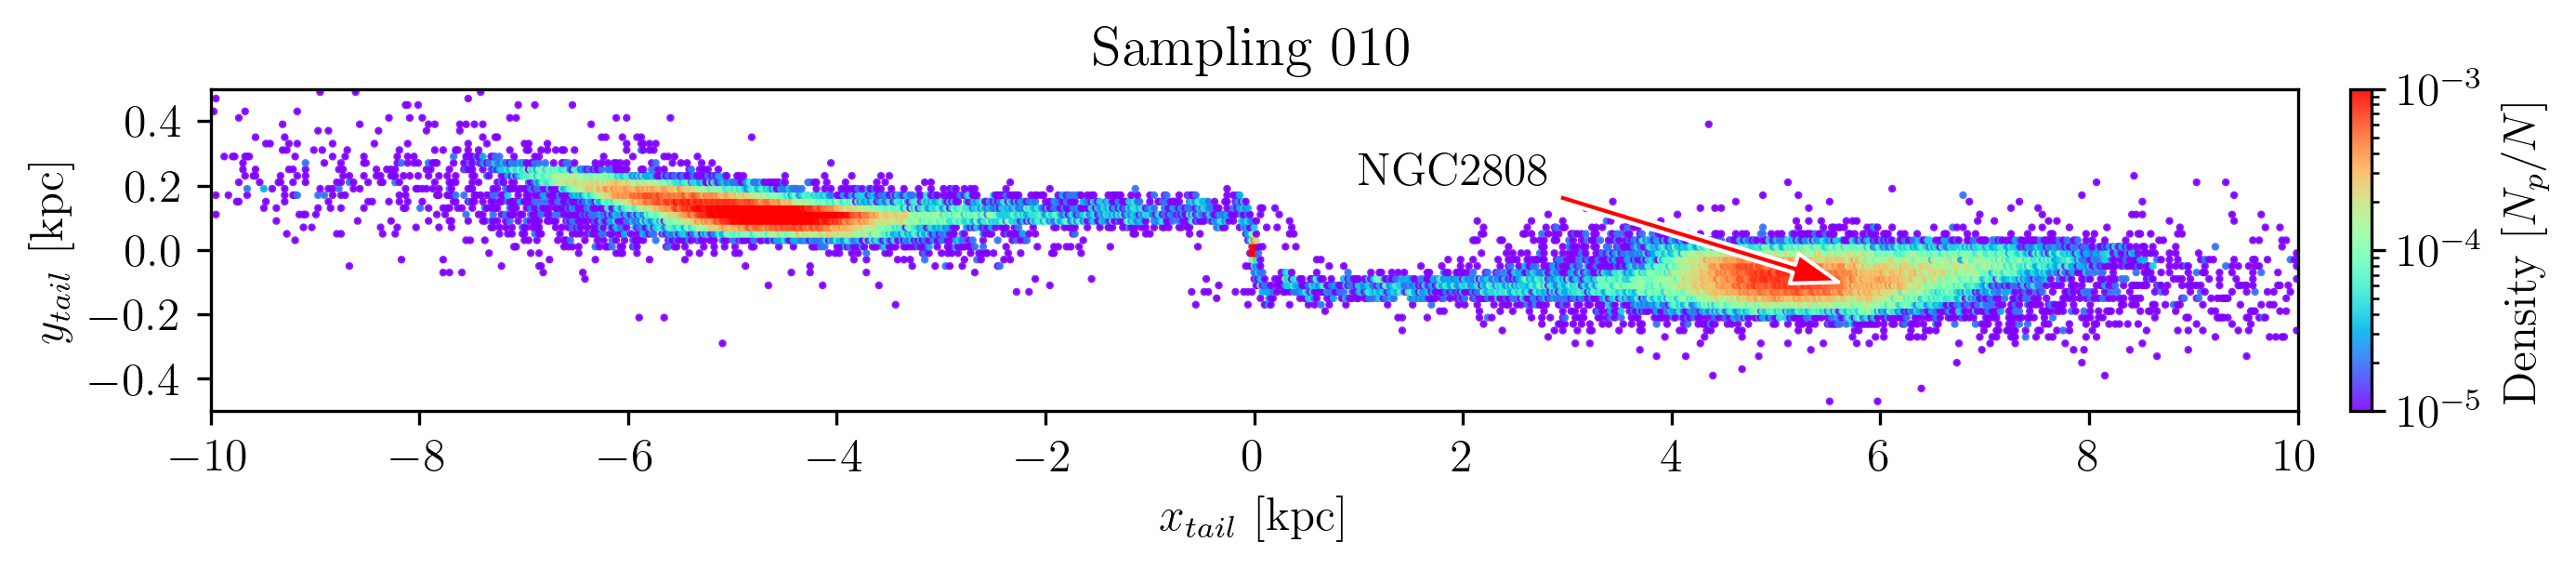
\includegraphics[width=\linewidth]{gallery_of_gaps_monte-carlo-010.png}
      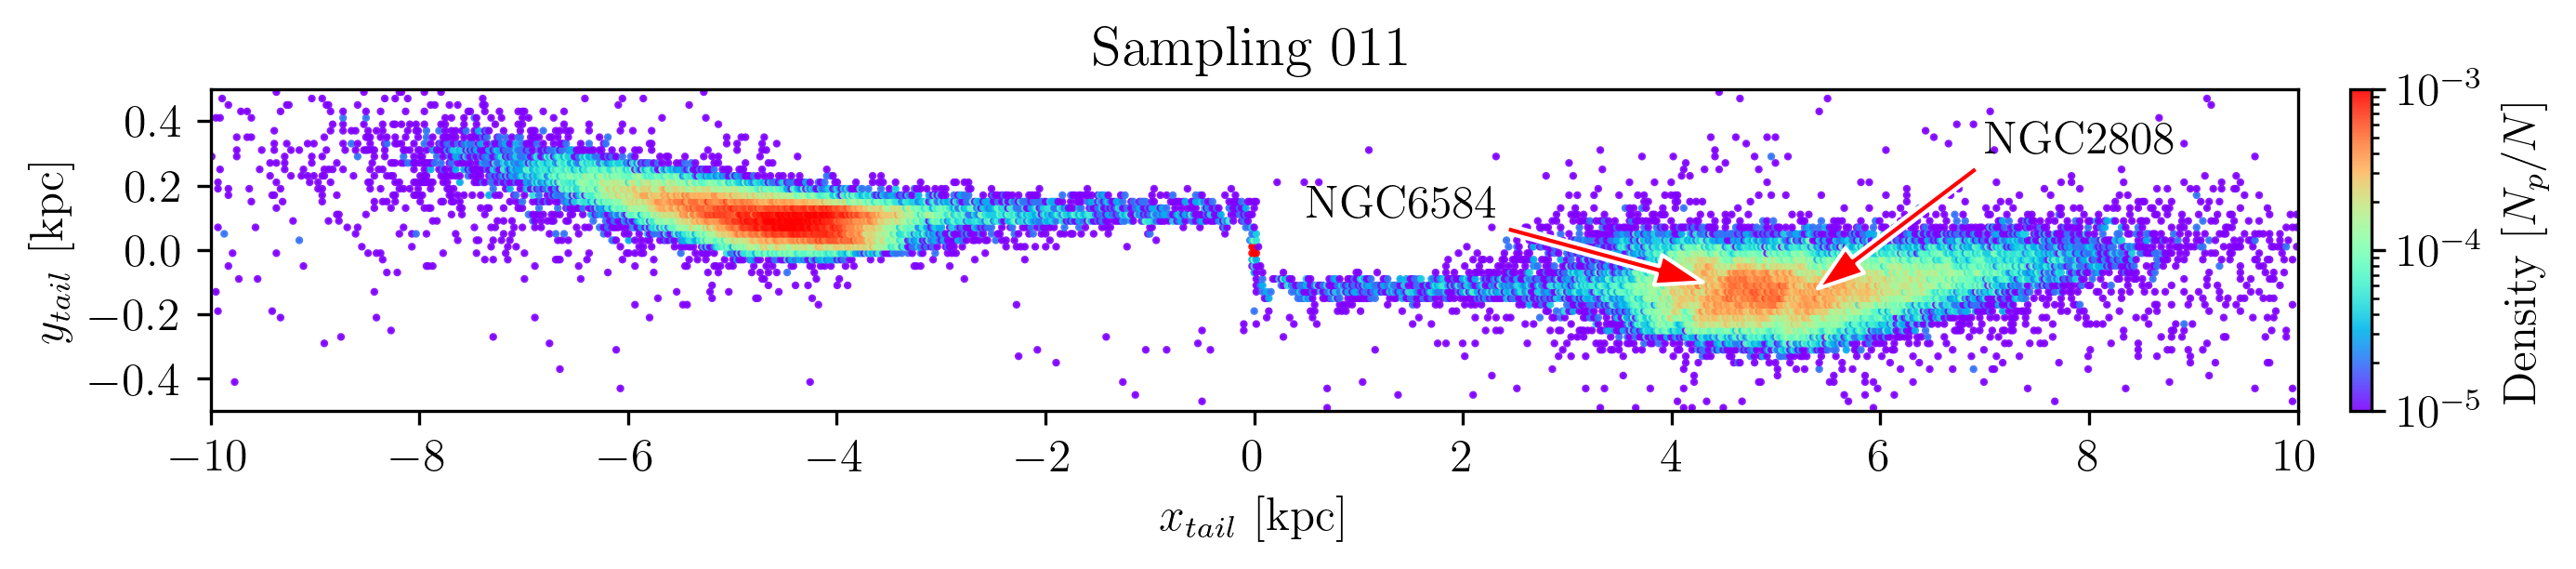
\includegraphics[width=\linewidth]{gallery_of_gaps_monte-carlo-011.png}
      \caption{Third gap gallery}
      \label{fig:gallery2}
      \end{figure*}

    \begin{figure*}
      \centering
      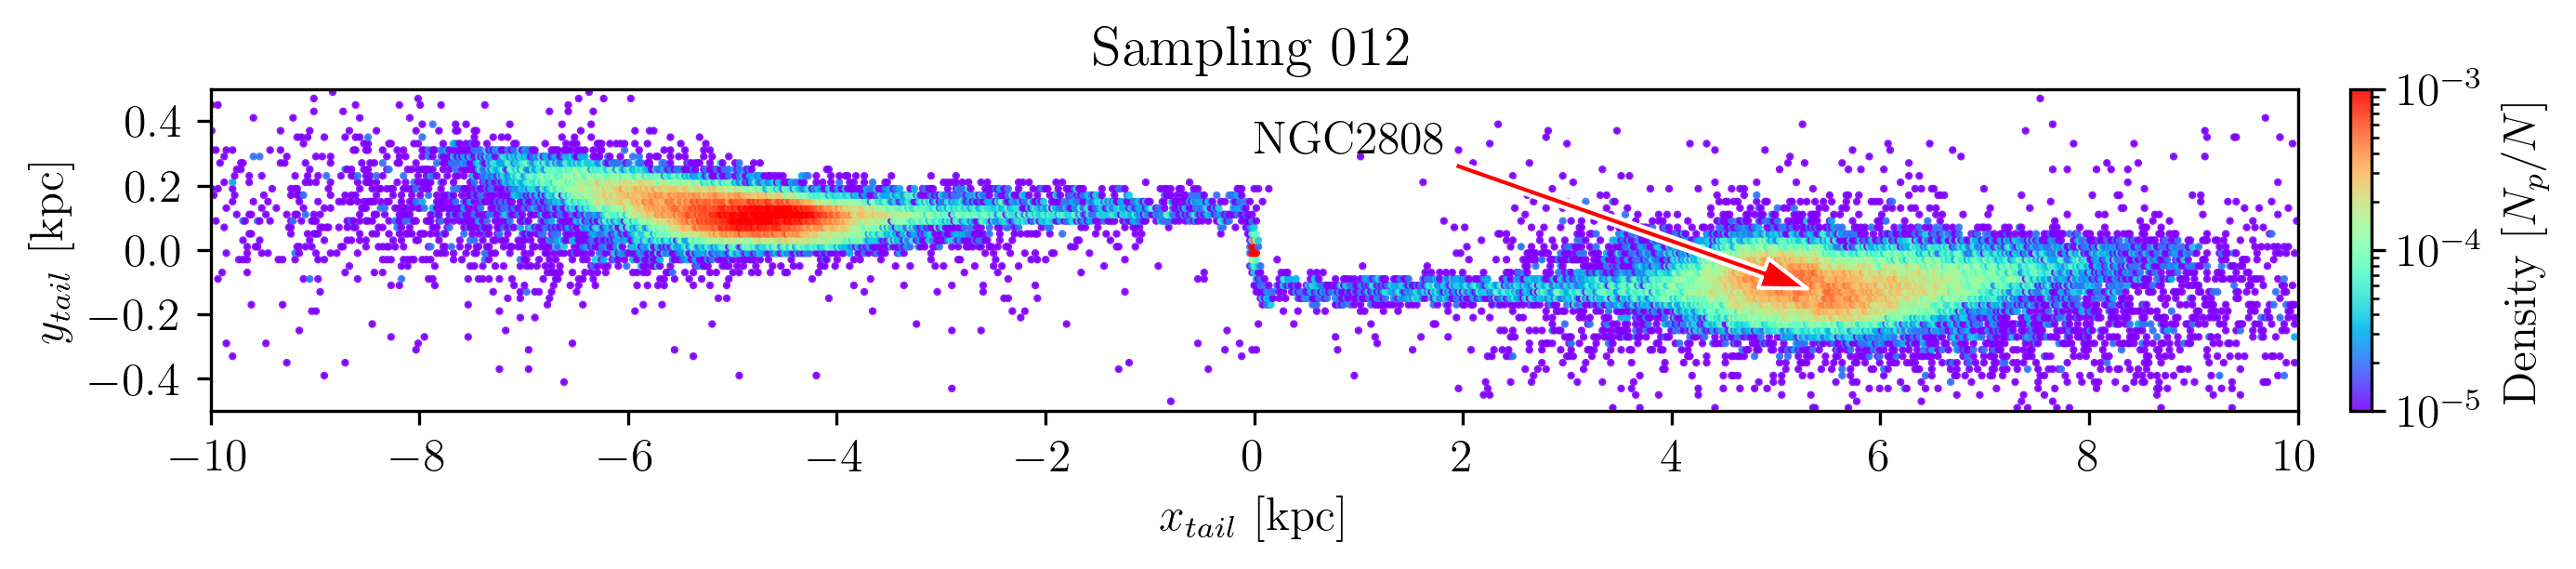
\includegraphics[width=\linewidth]{gallery_of_gaps_monte-carlo-012.png}
      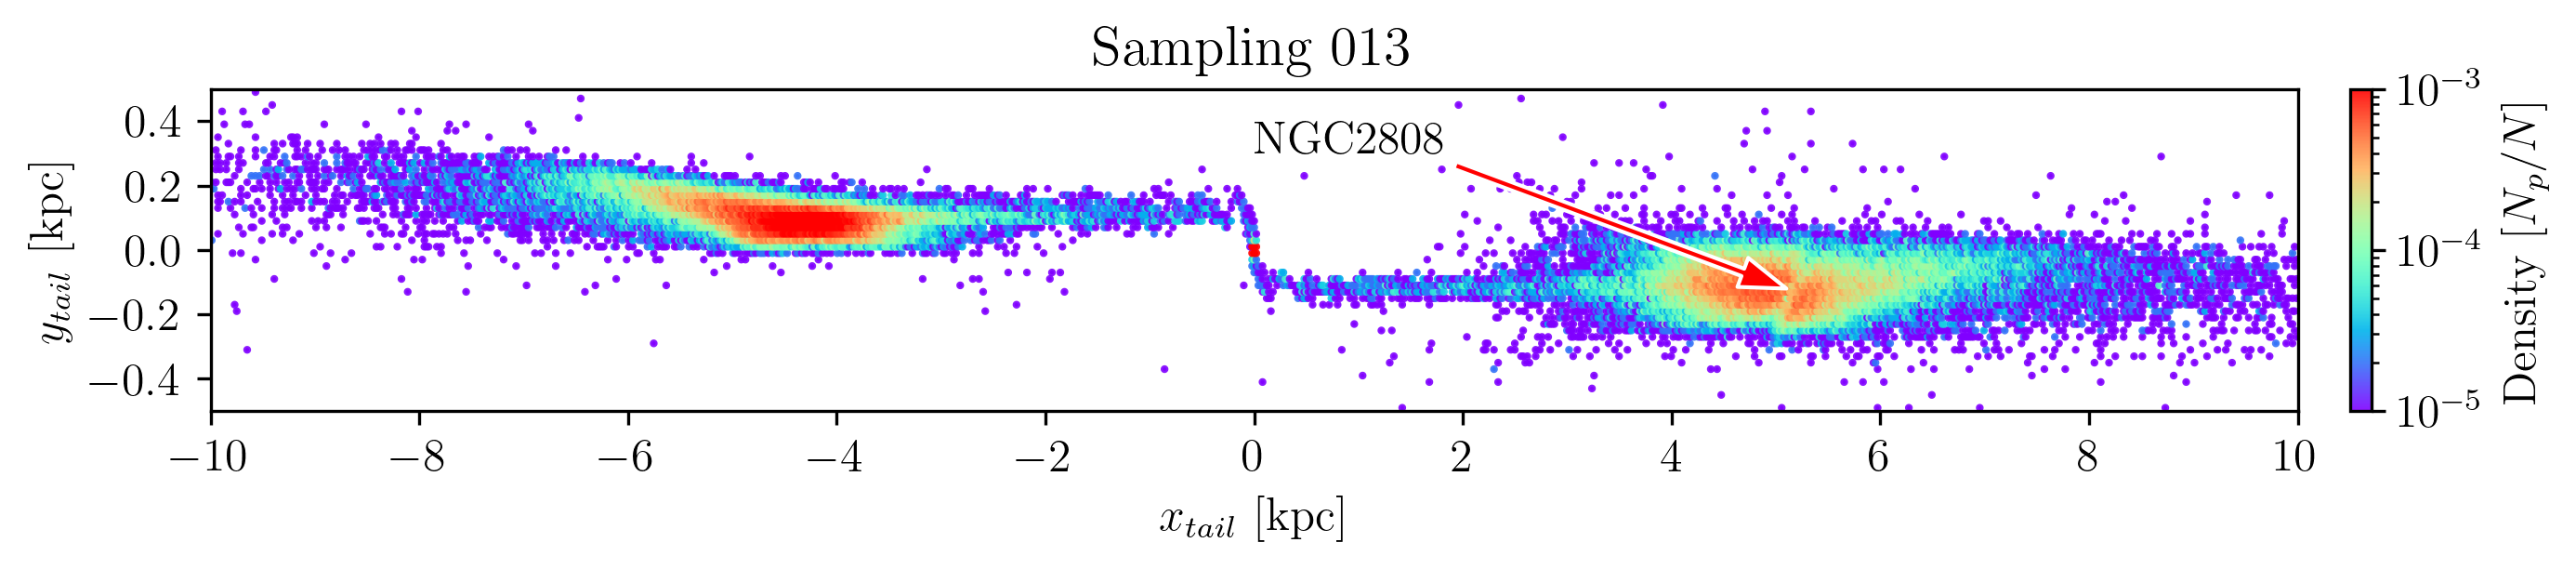
\includegraphics[width=\linewidth]{gallery_of_gaps_monte-carlo-013.png}
      
\includegraphics[width=\linewidth]{gallery_of_gaps_monte-carlo-014.png}      
      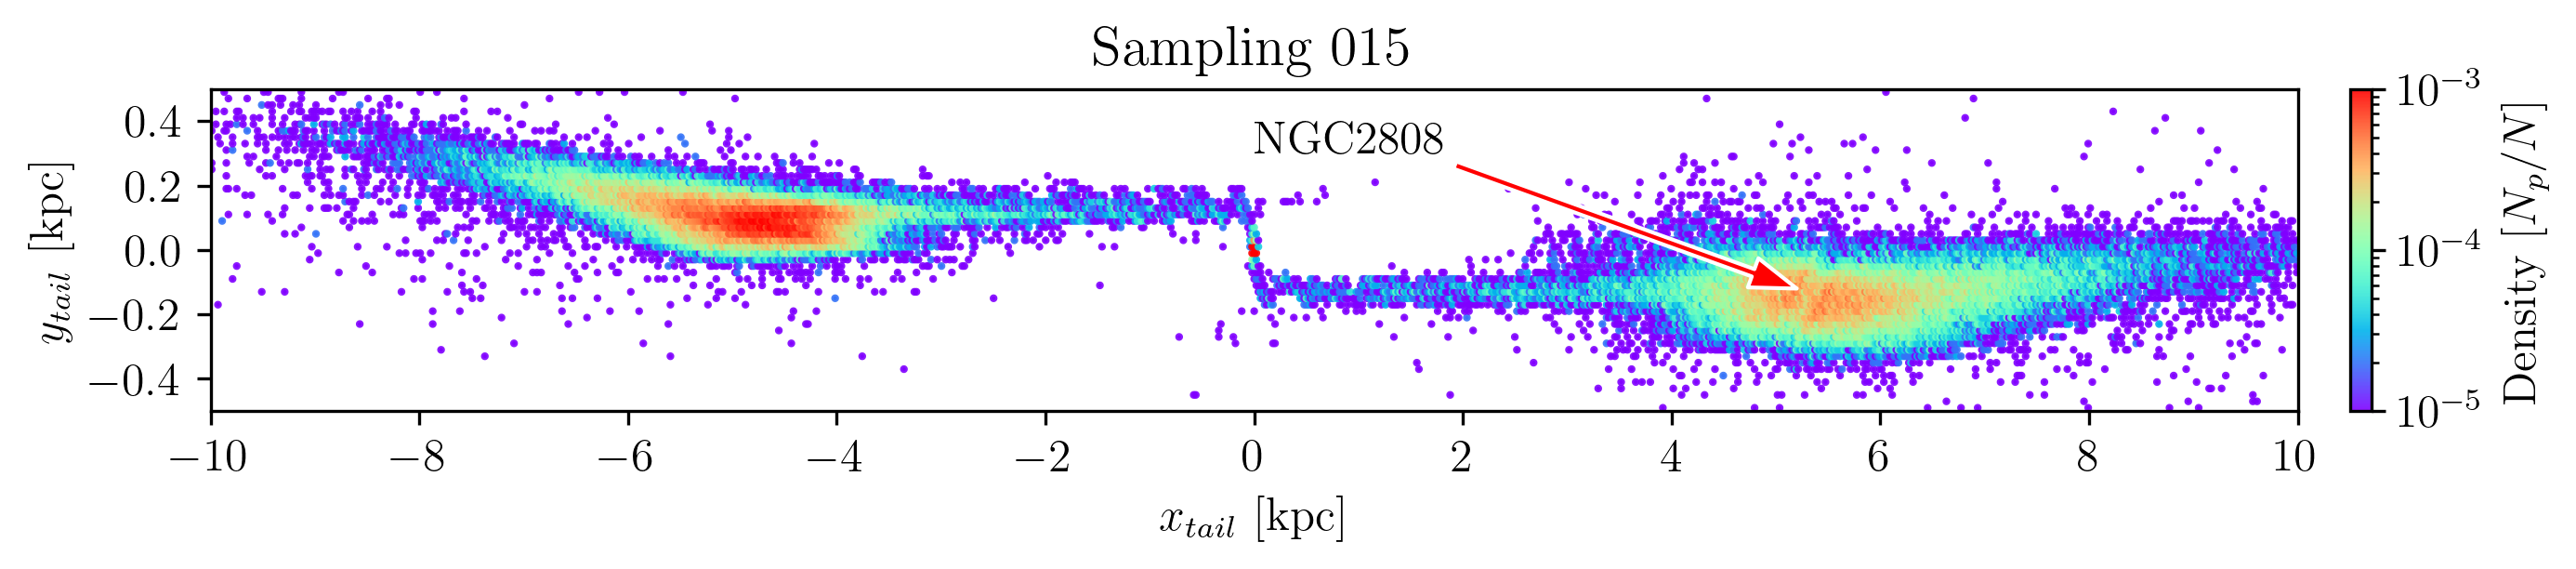
\includegraphics[width=\linewidth]{gallery_of_gaps_monte-carlo-015.png}
      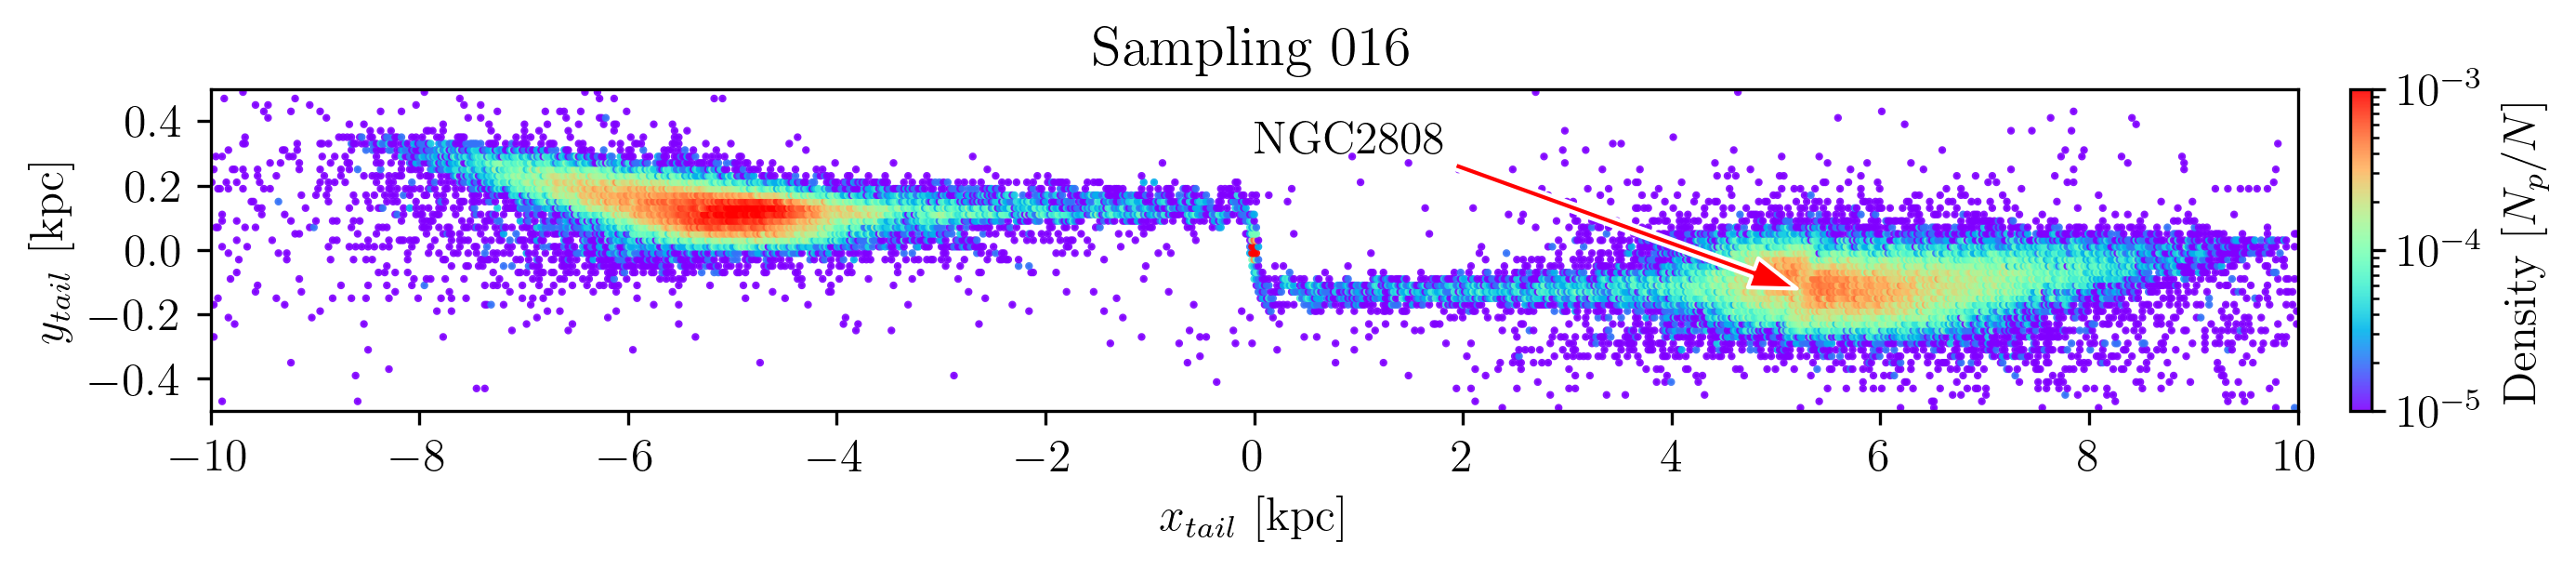
\includegraphics[width=\linewidth]{gallery_of_gaps_monte-carlo-016.png}
      \caption{Fourth gap gallery}
      \label{fig:gallery3}
      \end{figure*}

    \begin{figure*}
      \centering
      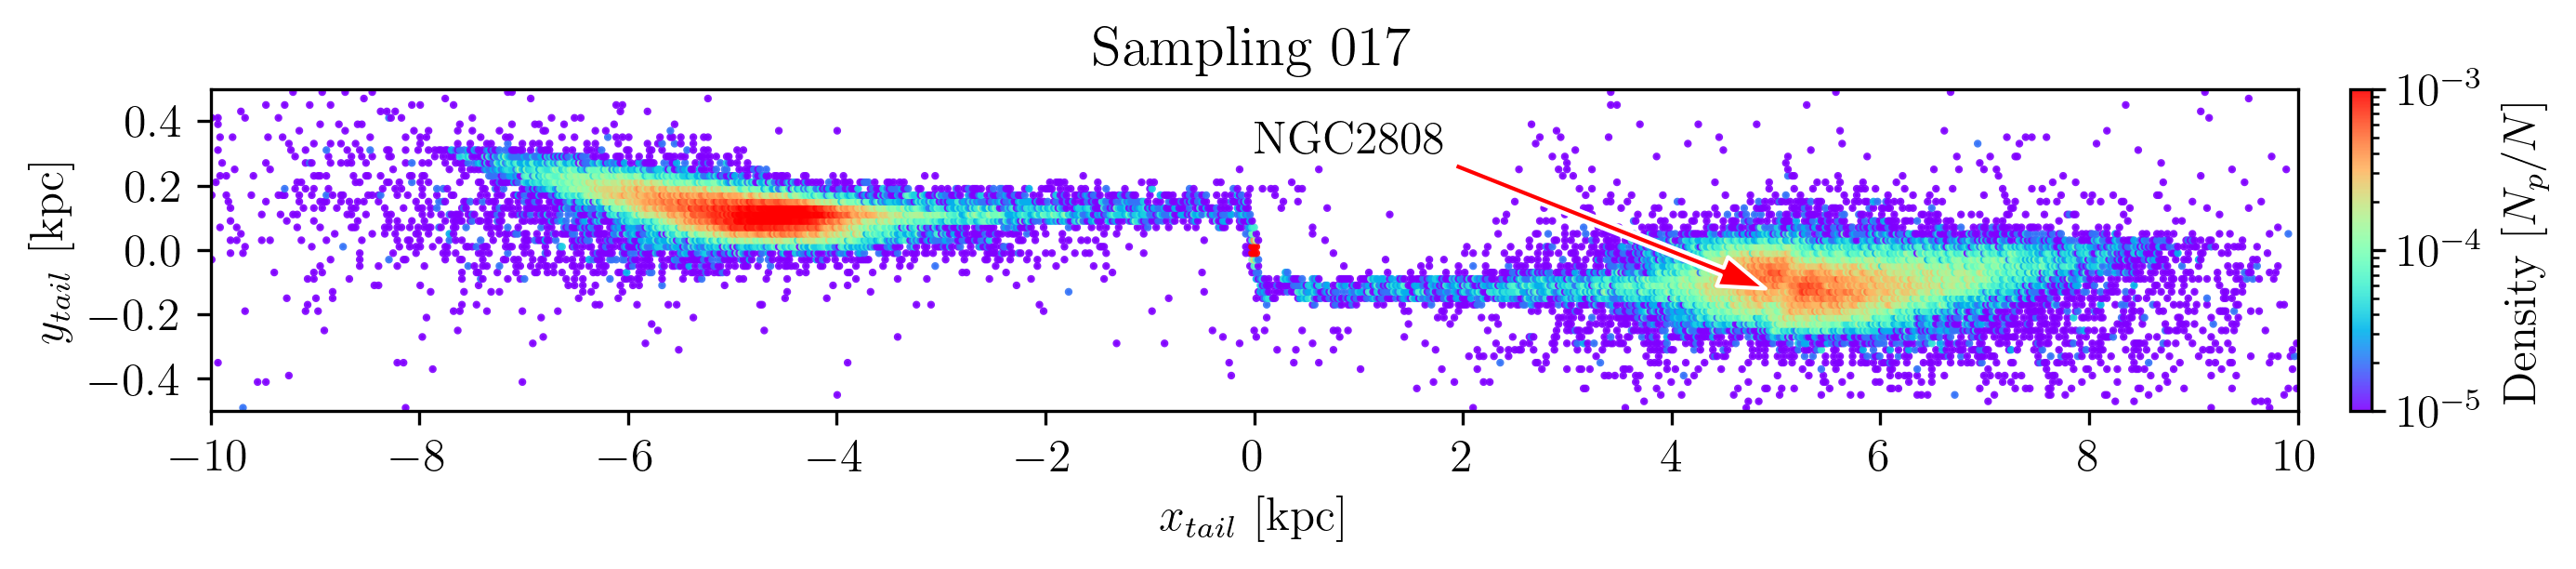
\includegraphics[width=\linewidth]{gallery_of_gaps_monte-carlo-017.png}
      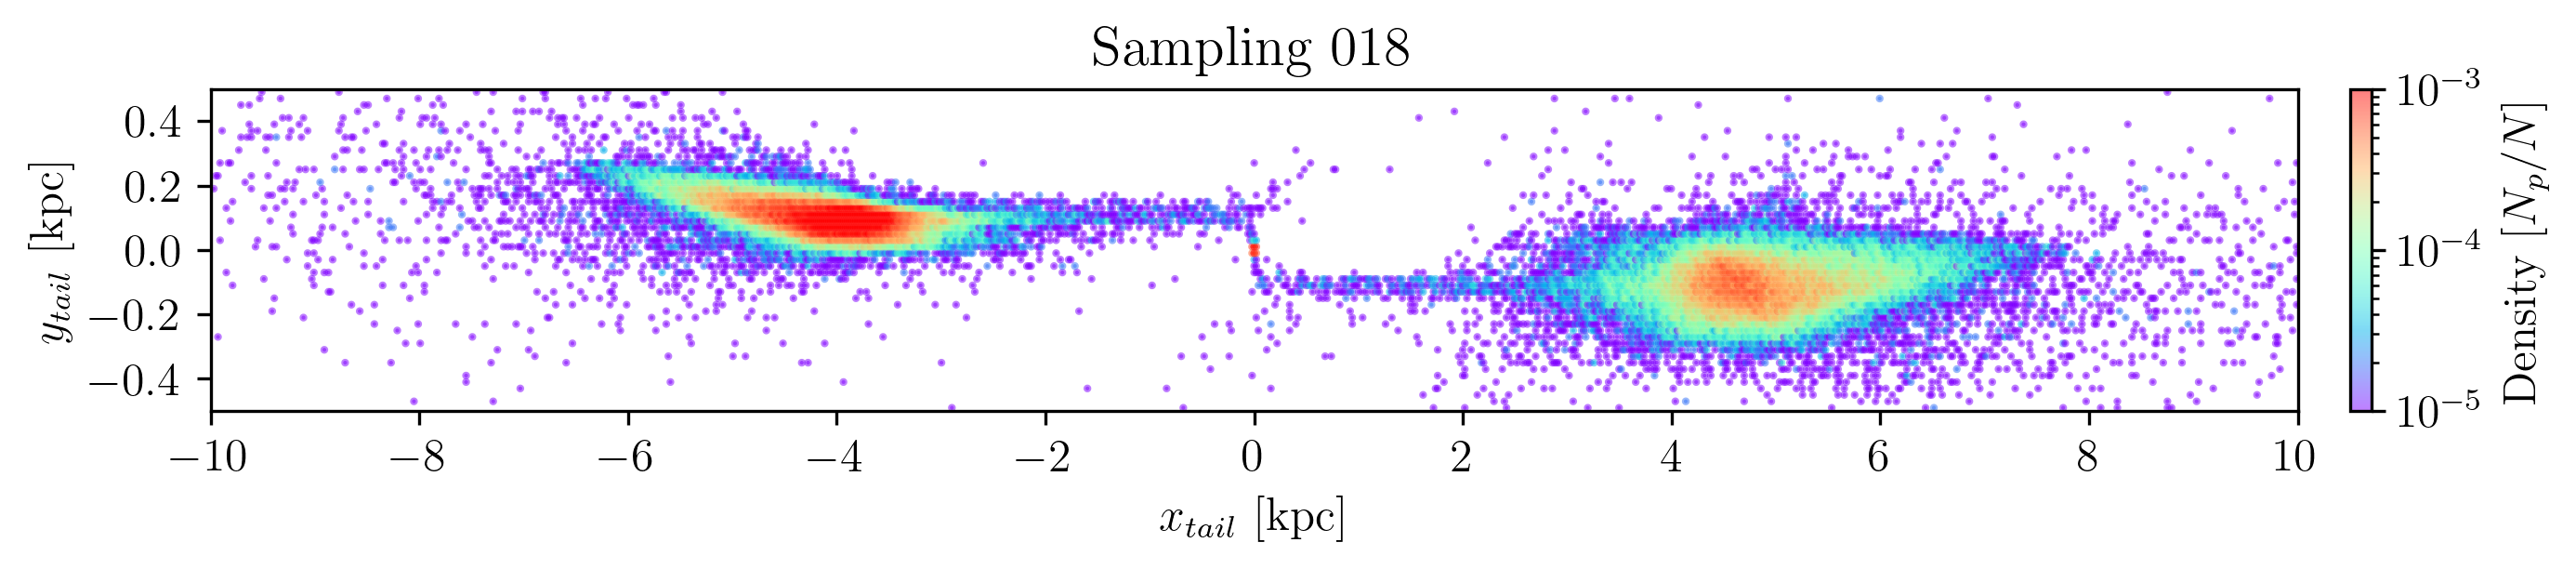
\includegraphics[width=\linewidth]{gallery_of_gaps_monte-carlo-018.png}
      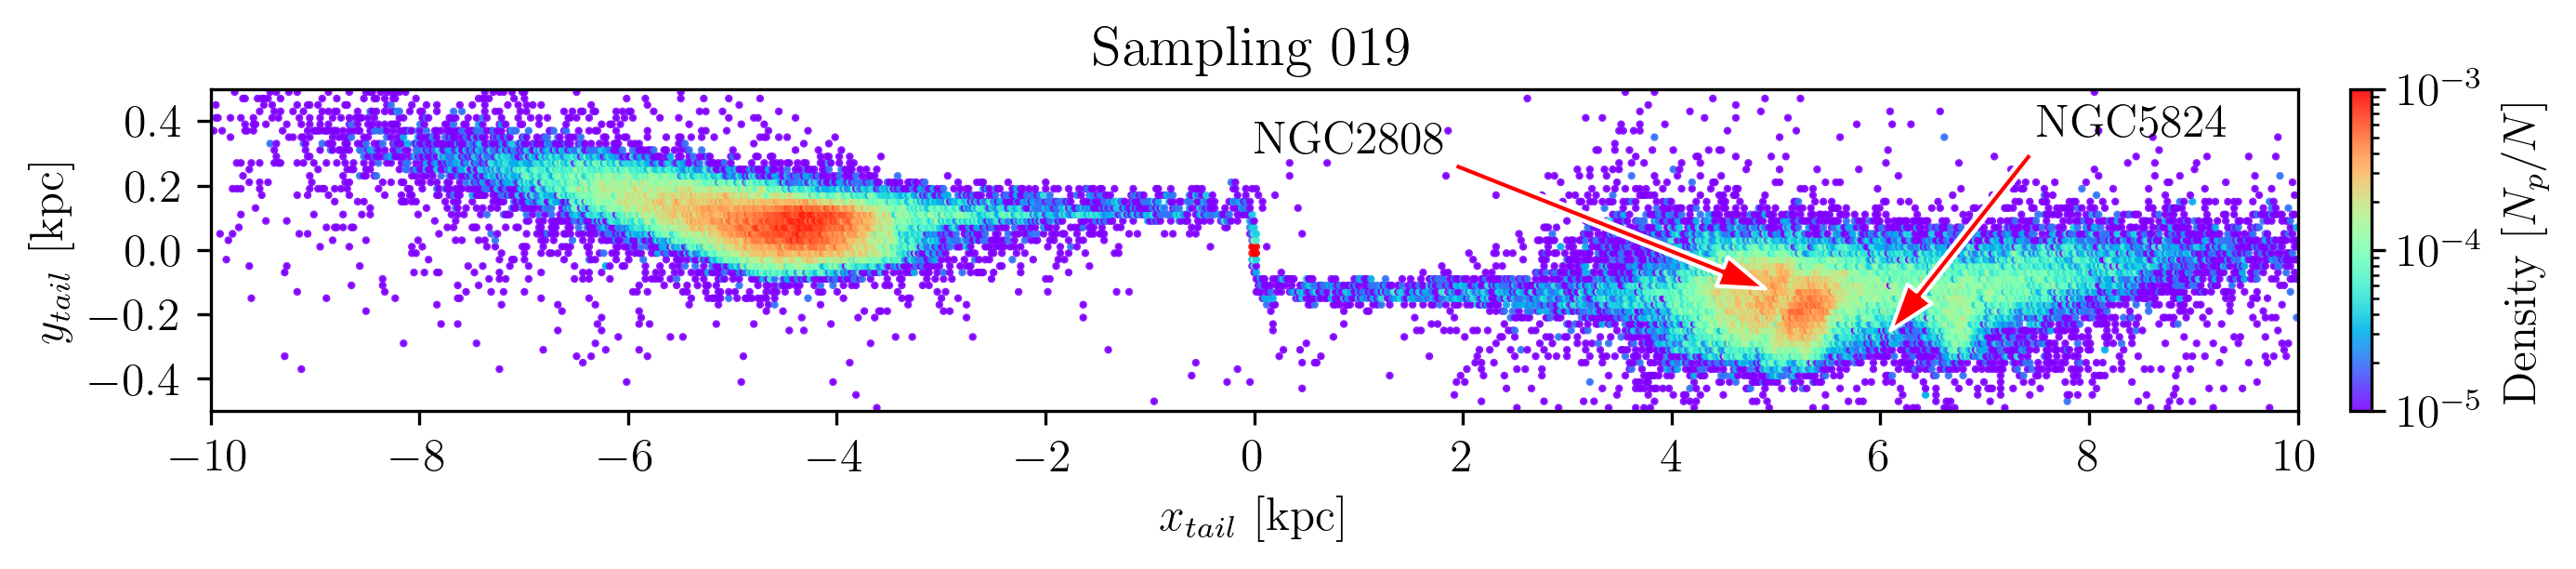
\includegraphics[width=\linewidth]{gallery_of_gaps_monte-carlo-019.png}      
      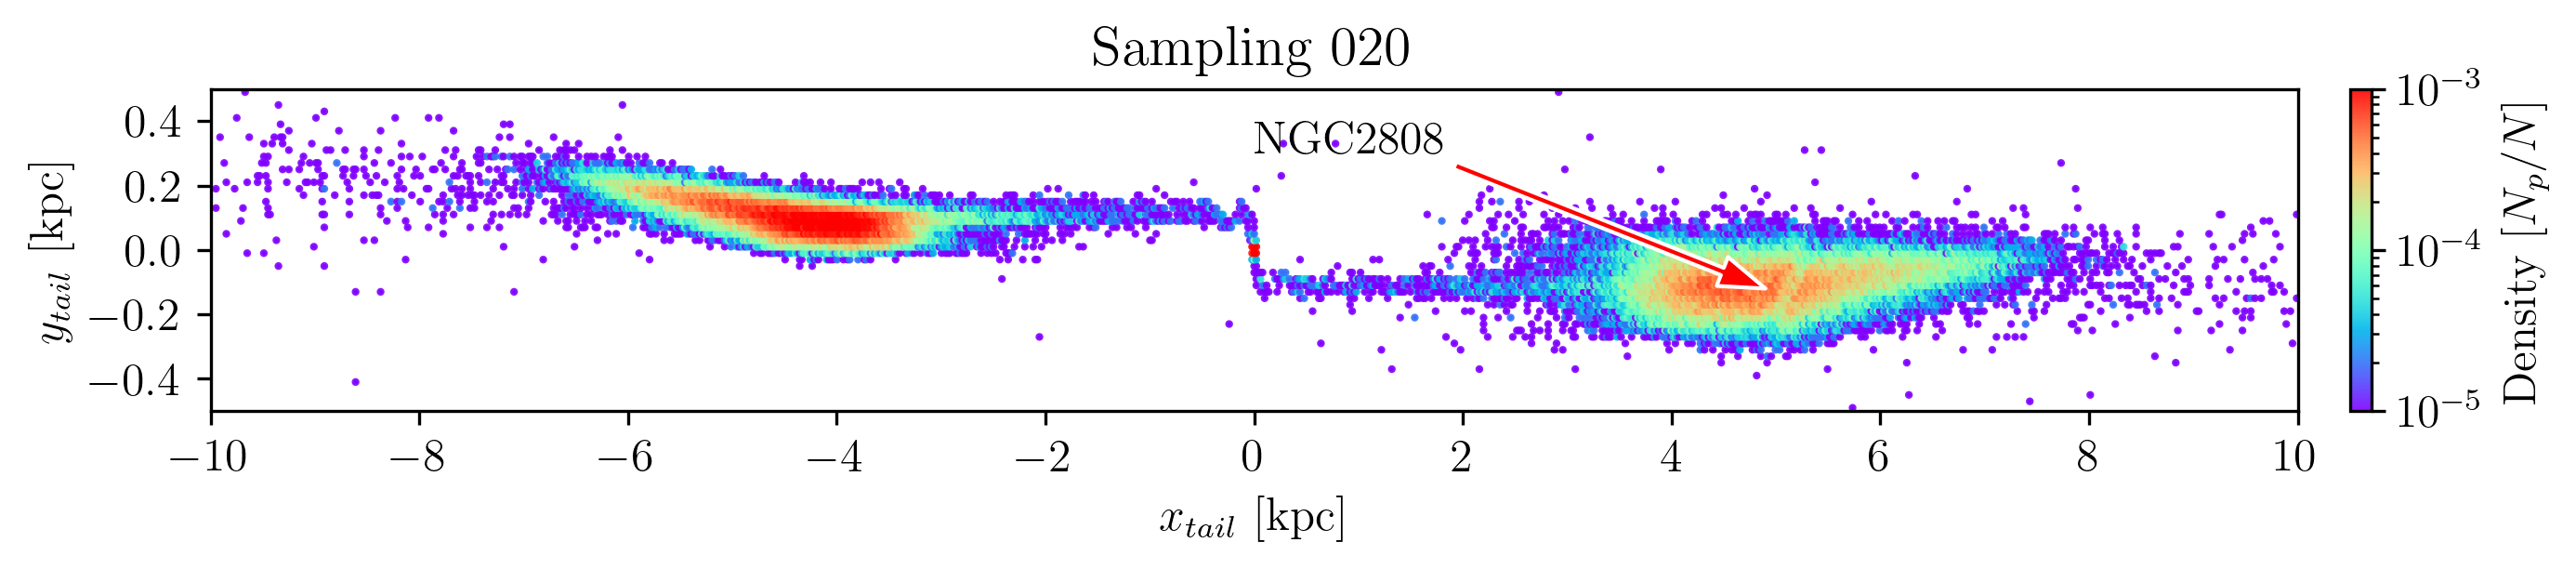
\includegraphics[width=\linewidth]{gallery_of_gaps_monte-carlo-020.png}
      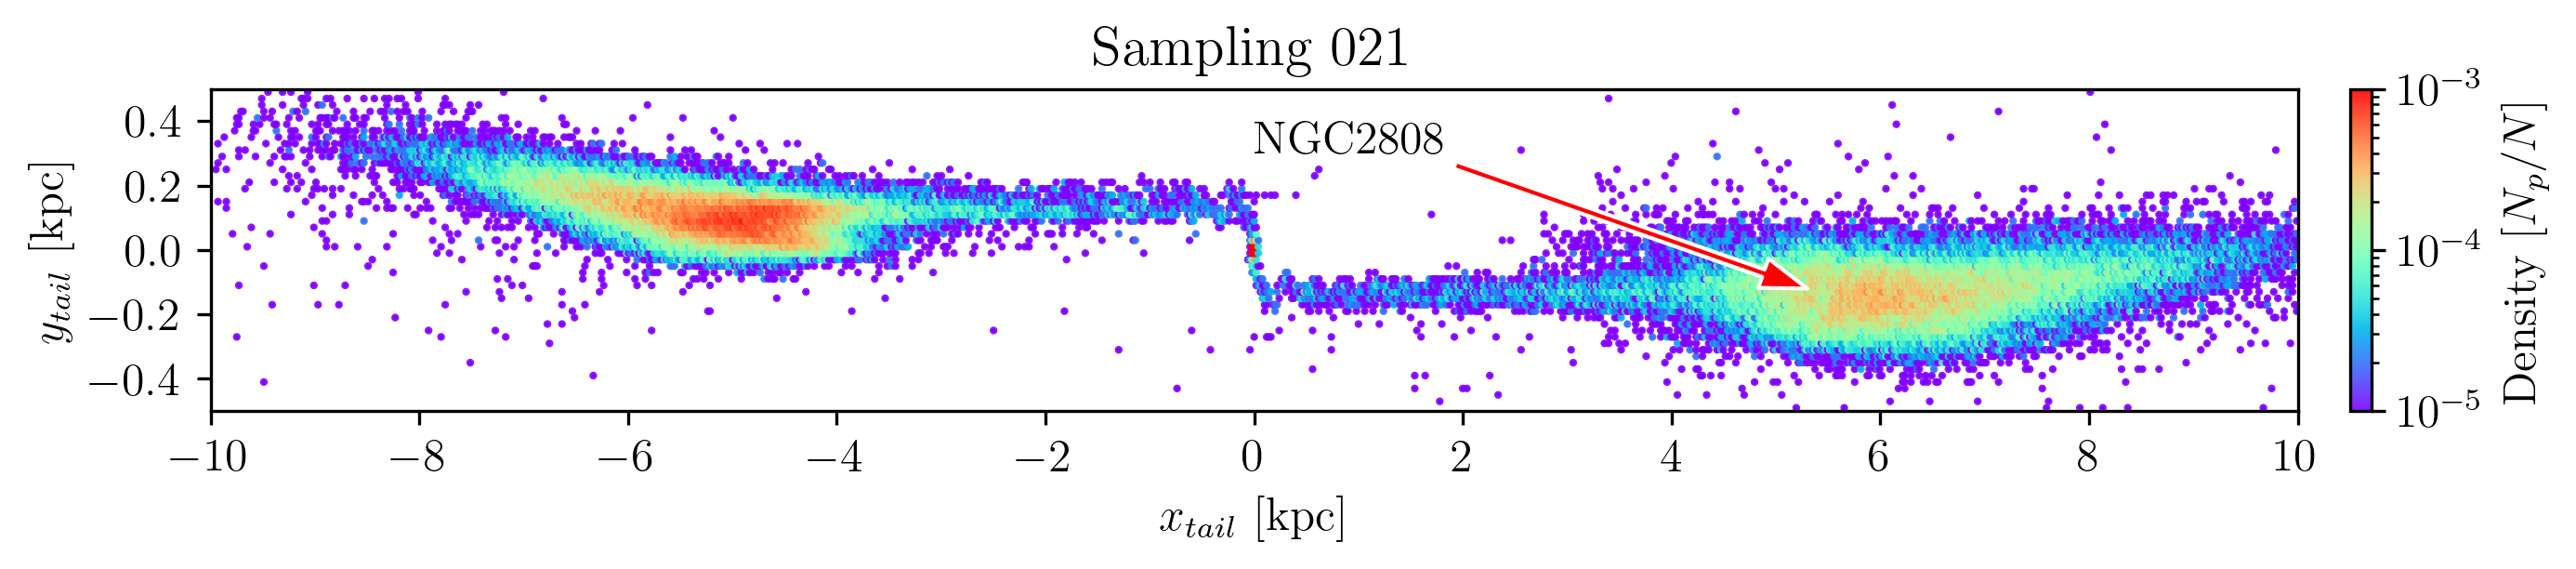
\includegraphics[width=\linewidth]{gallery_of_gaps_monte-carlo-021.png}
      \caption{Fifth gap gallery}
      \label{fig:gallery4}
      \end{figure*}

    \begin{figure*}
      \centering
      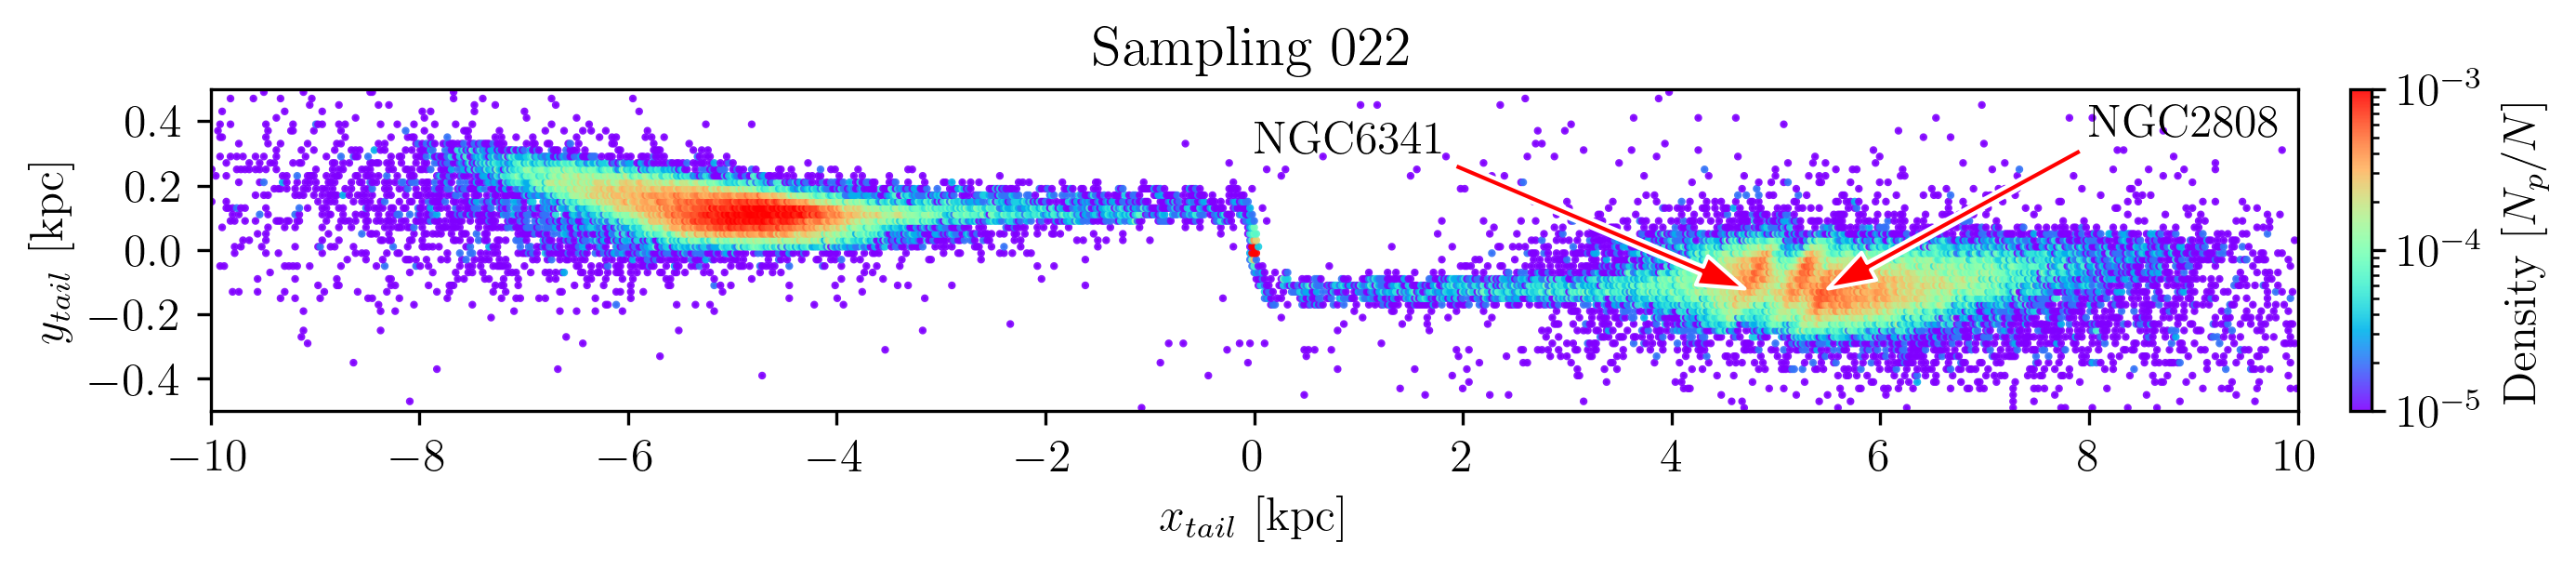
\includegraphics[width=\linewidth]{gallery_of_gaps_monte-carlo-022.png}
      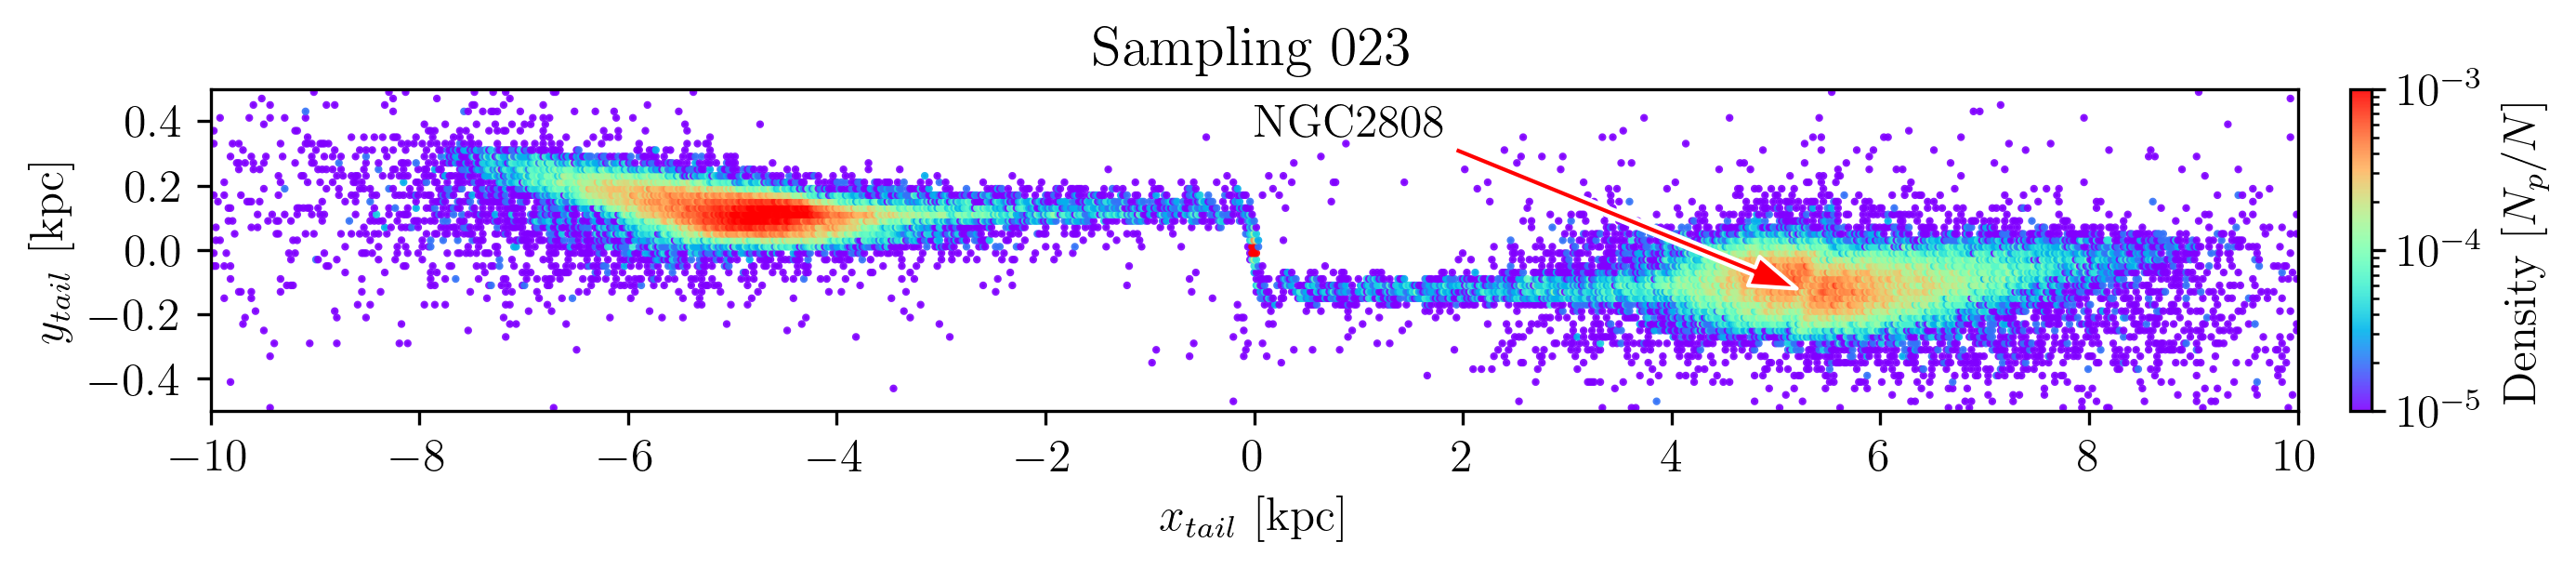
\includegraphics[width=\linewidth]{gallery_of_gaps_monte-carlo-023.png}
      
\includegraphics[width=\linewidth]{gallery_of_gaps_monte-carlo-024.png}   
      
\includegraphics[width=\linewidth]{tau-profile-monte-carlo-024.png}
      
\includegraphics[width=\linewidth]{gallery_of_gaps_monte-carlo-025.png}
      \caption{Sixth gap gallery}
      \label{fig:gallery5}
      \end{figure*}

    \begin{figure*}
      \centering
      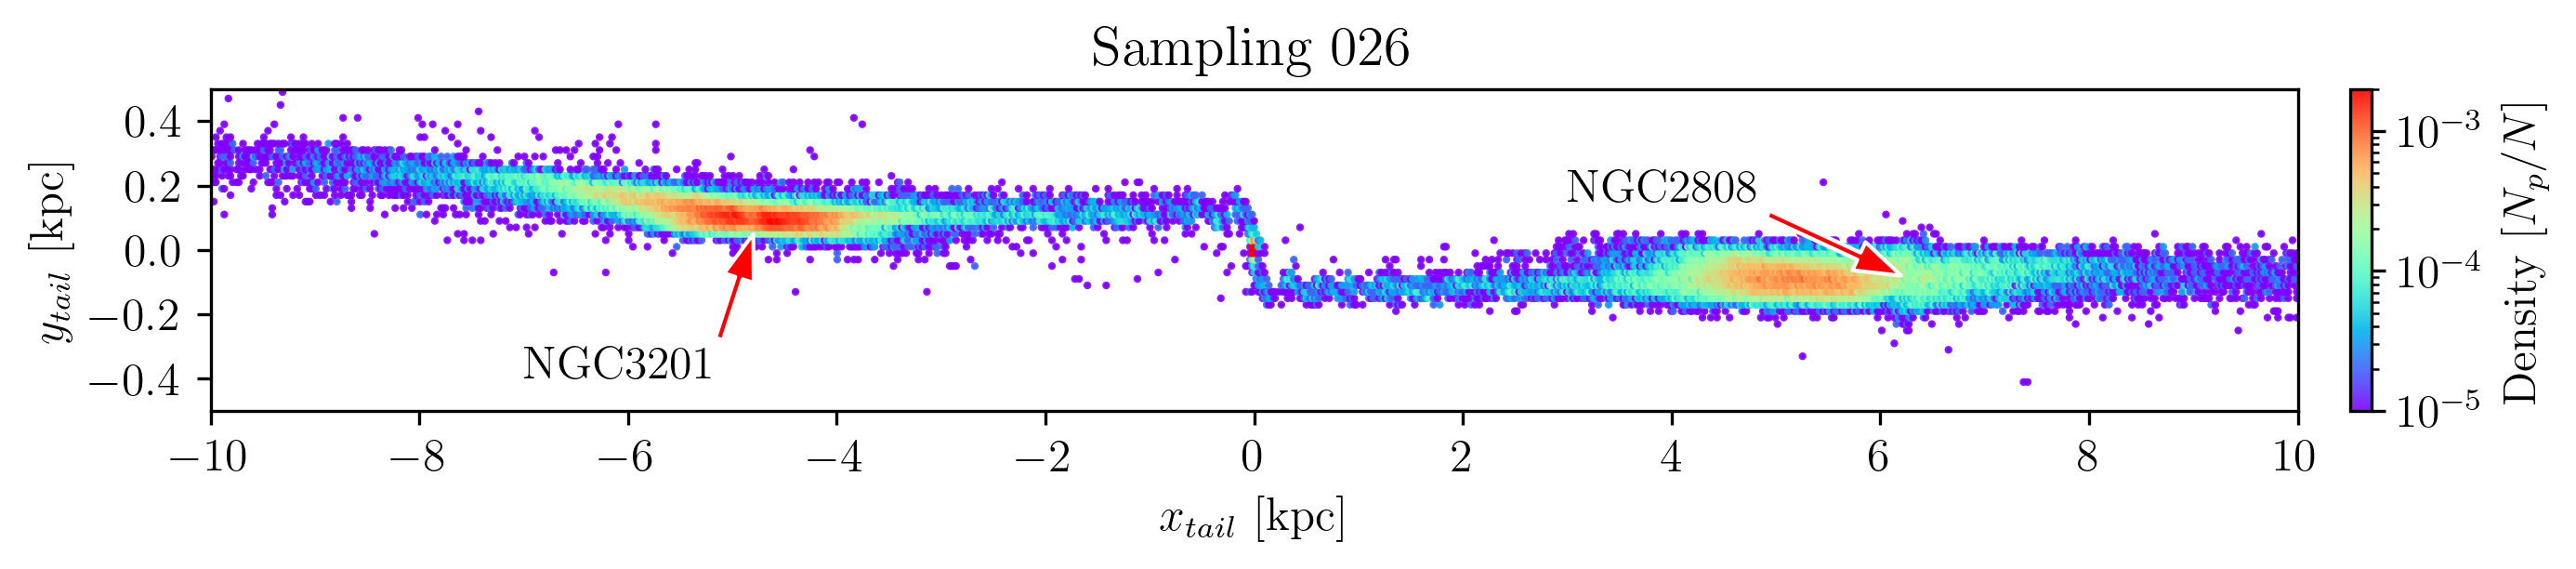
\includegraphics[width=\linewidth]{gallery_of_gaps_monte-carlo-026.png}
      
\includegraphics[width=\linewidth]{gallery_of_gaps_monte-carlo-027.png}
      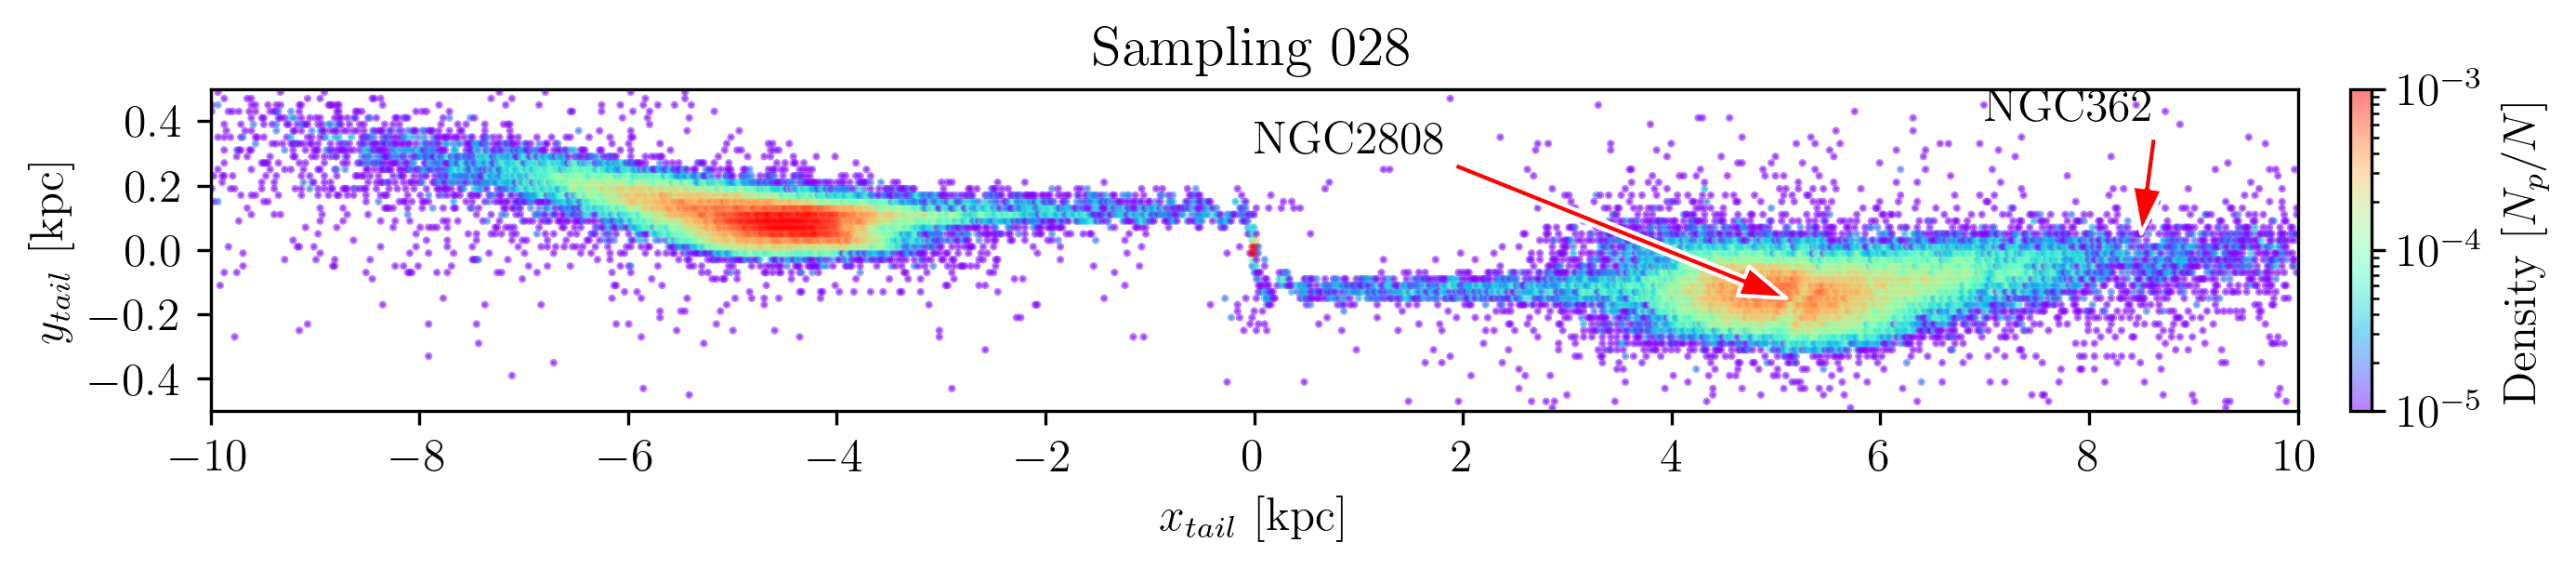
\includegraphics[width=\linewidth]{gallery_of_gaps_monte-carlo-028.png}
      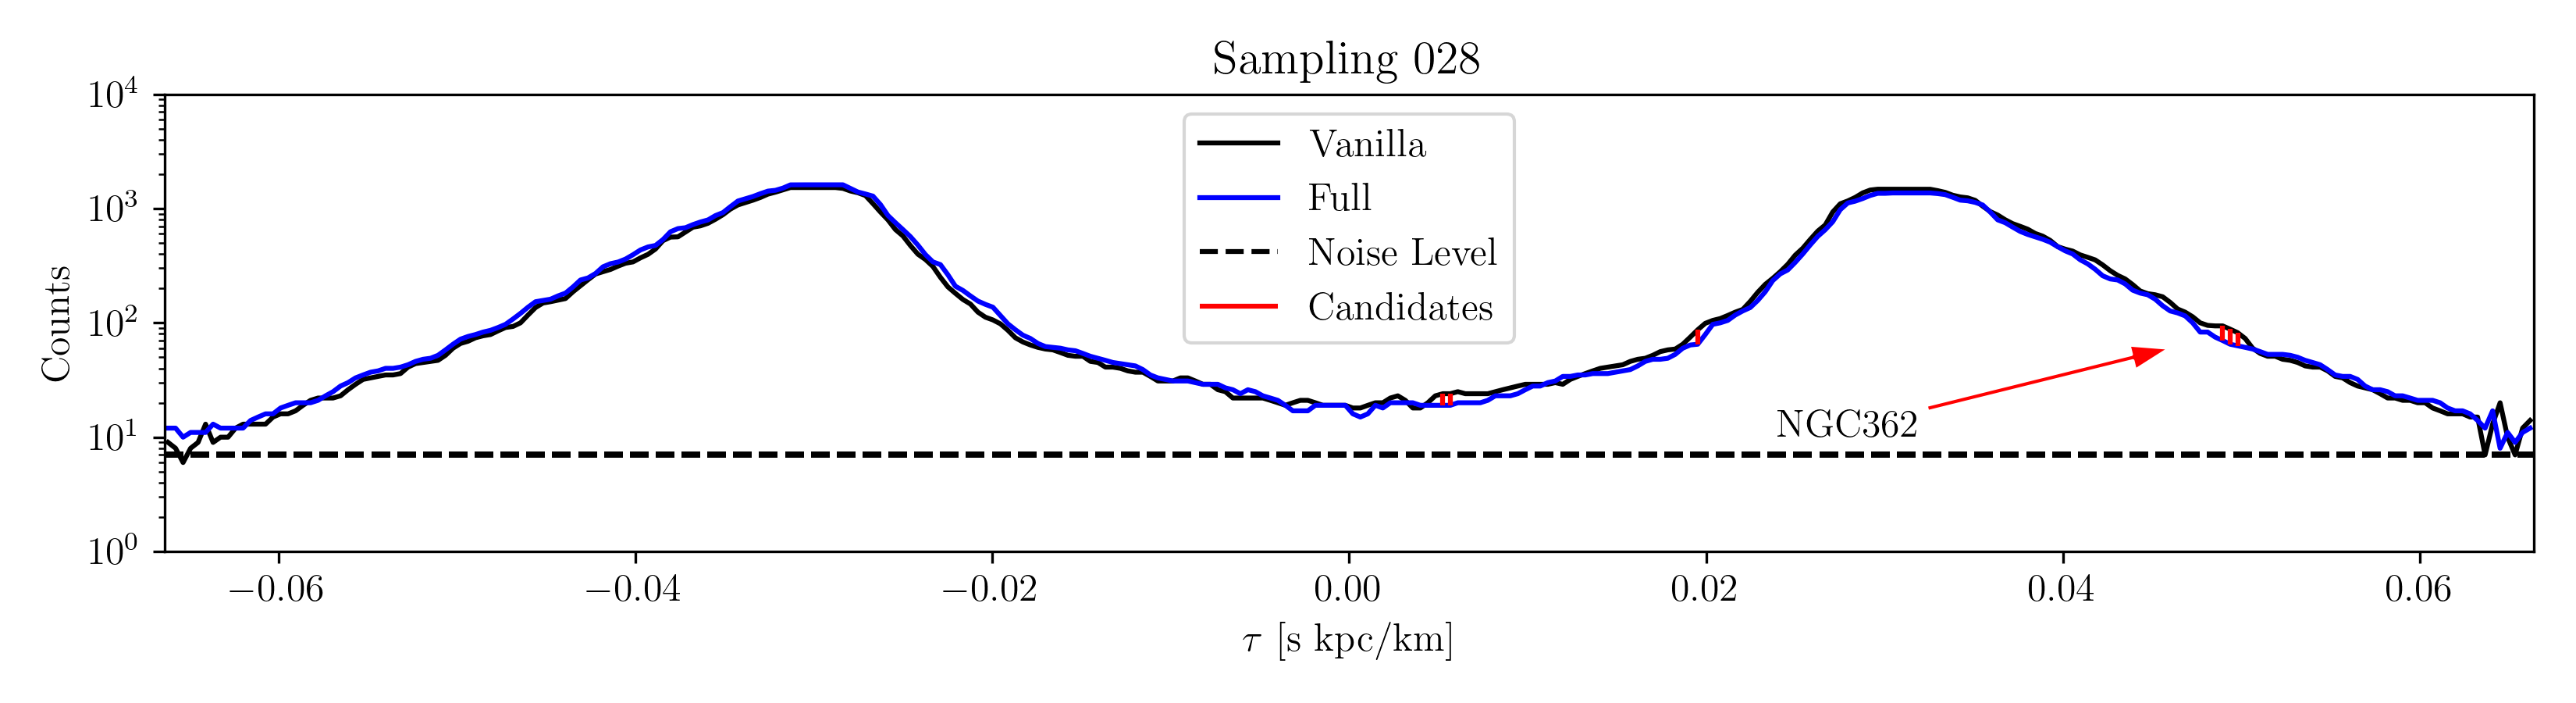
\includegraphics[width=\linewidth]{tau-profile-monte-carlo-028.png}
      \caption{Seventh gap gallery}
      \label{fig:gallery6}
      \end{figure*}

    \begin{figure*}
      \centering      
      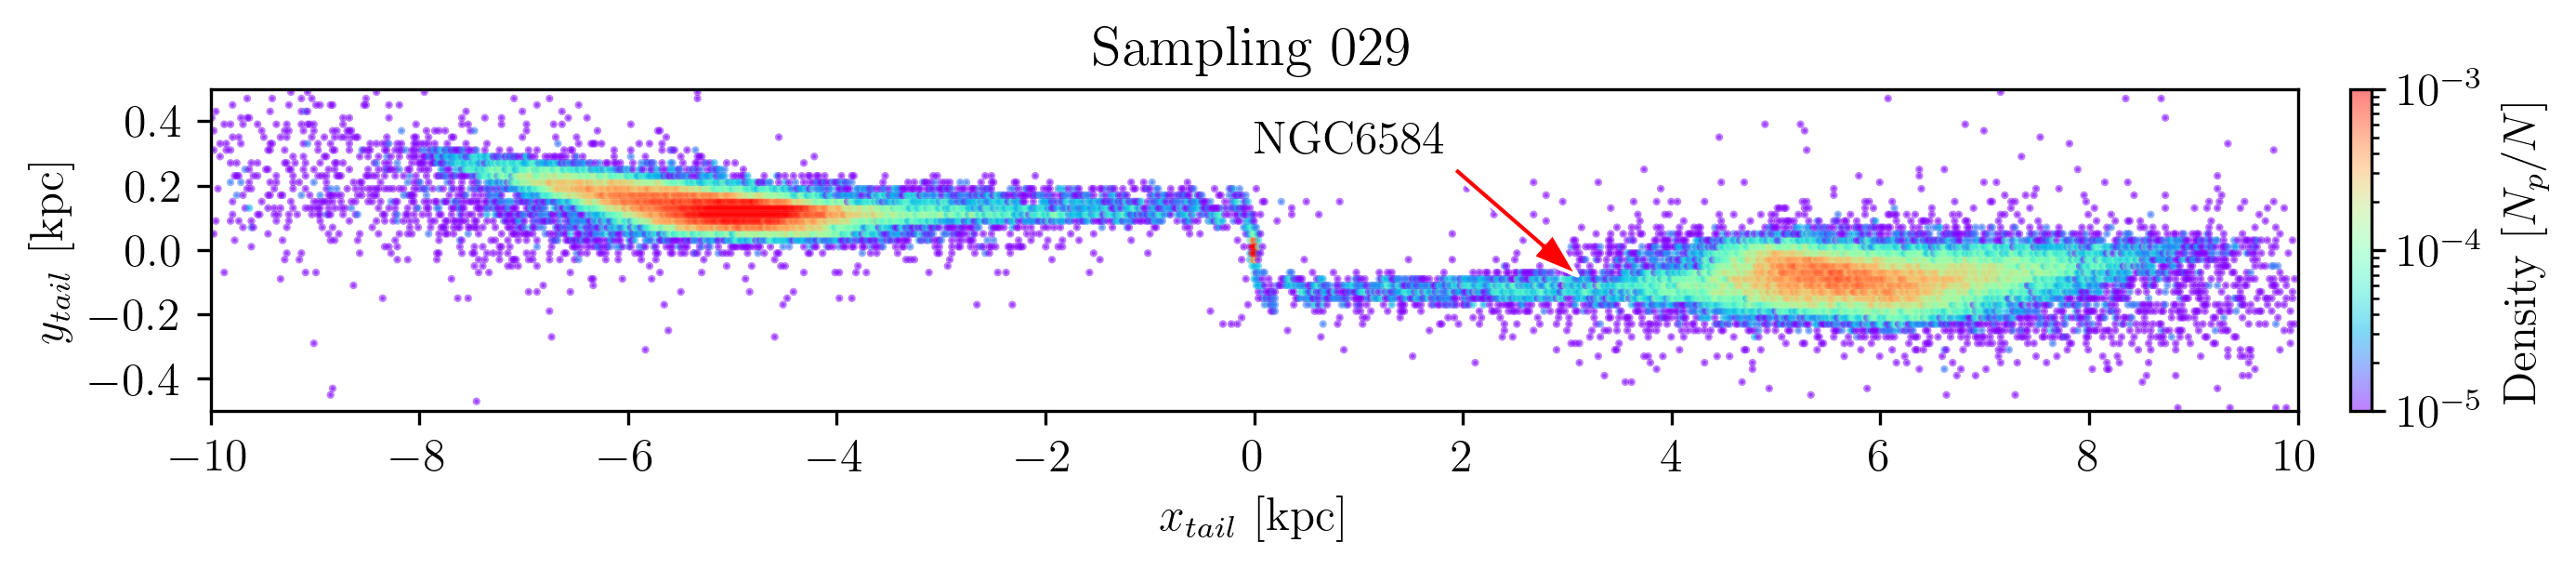
\includegraphics[width=\linewidth]{gallery_of_gaps_monte-carlo-029.png}    
      
\includegraphics[width=\linewidth]{tau-profile-monte-carlo-029.png}  
      
\includegraphics[width=\linewidth]{gallery_of_gaps_monte-carlo-030.png}
      
\includegraphics[width=\linewidth]{tau-profile-monte-carlo-030.png}
      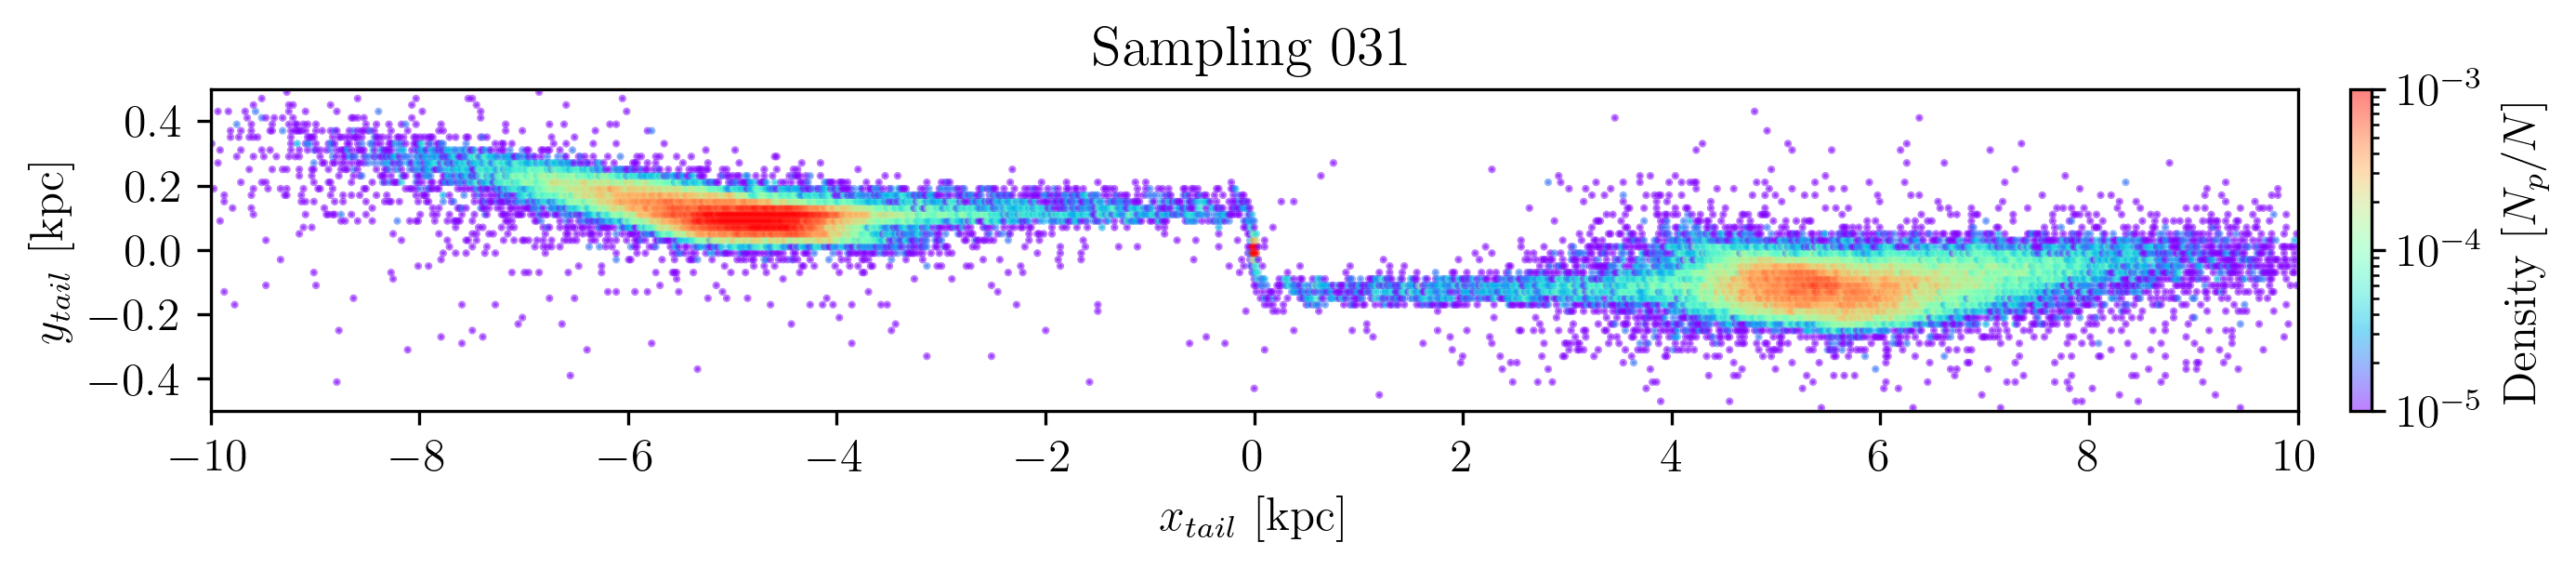
\includegraphics[width=\linewidth]{gallery_of_gaps_monte-carlo-031.png}
      \caption{Eighth gap gallery}
      \label{fig:gallery7}
      \end{figure*}

    \begin{figure*}
      \centering
      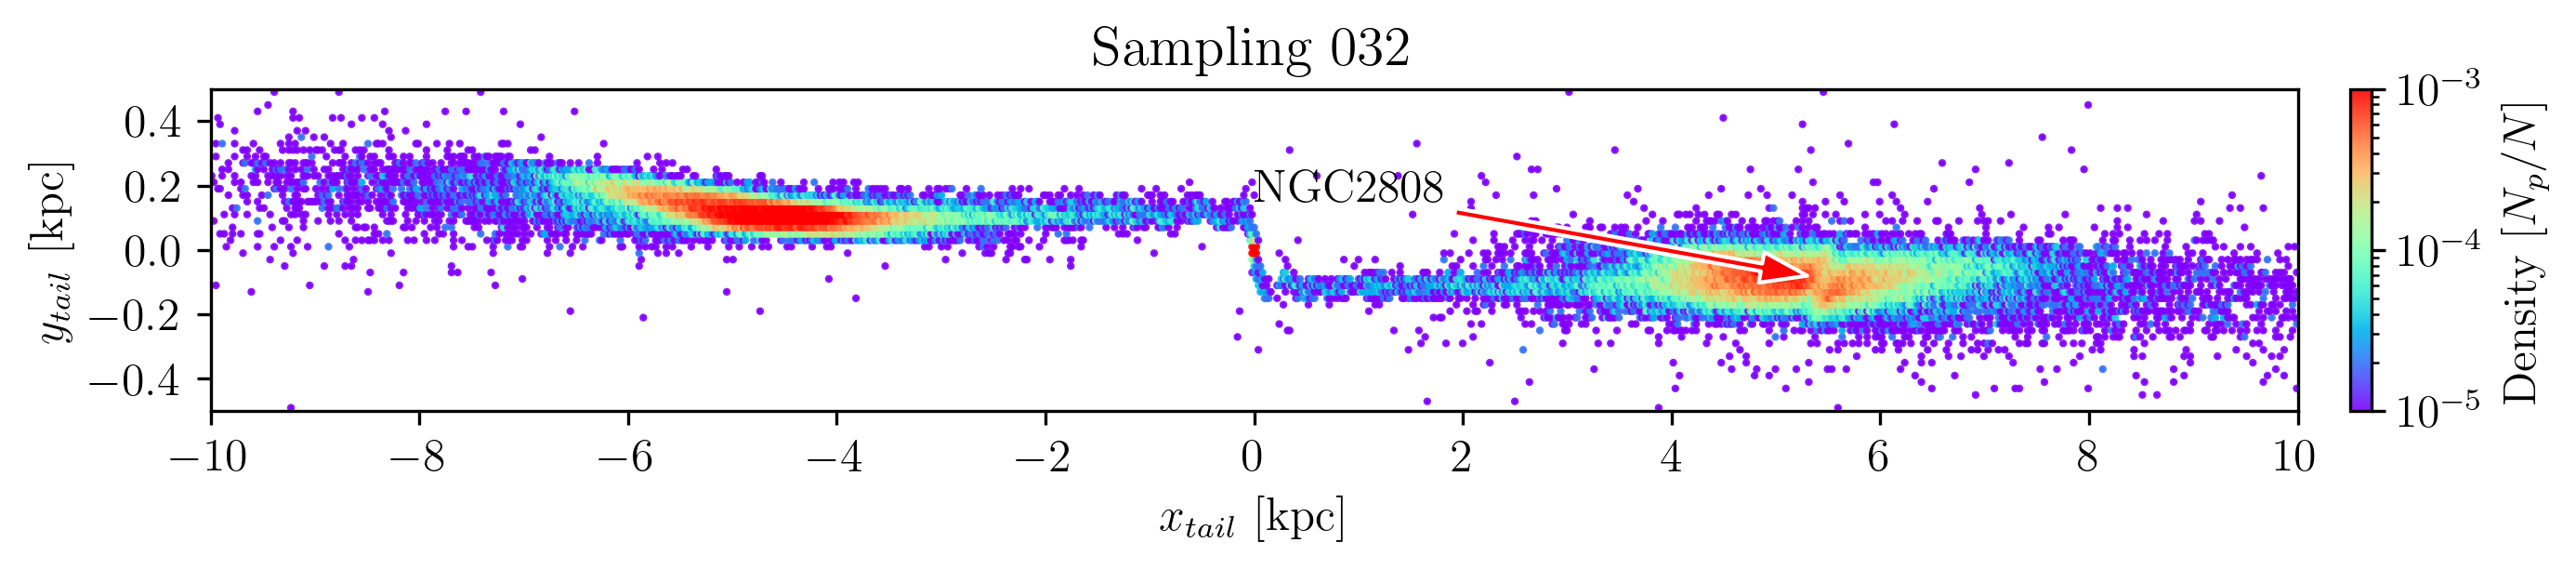
\includegraphics[width=\linewidth]{gallery_of_gaps_monte-carlo-032.png}
      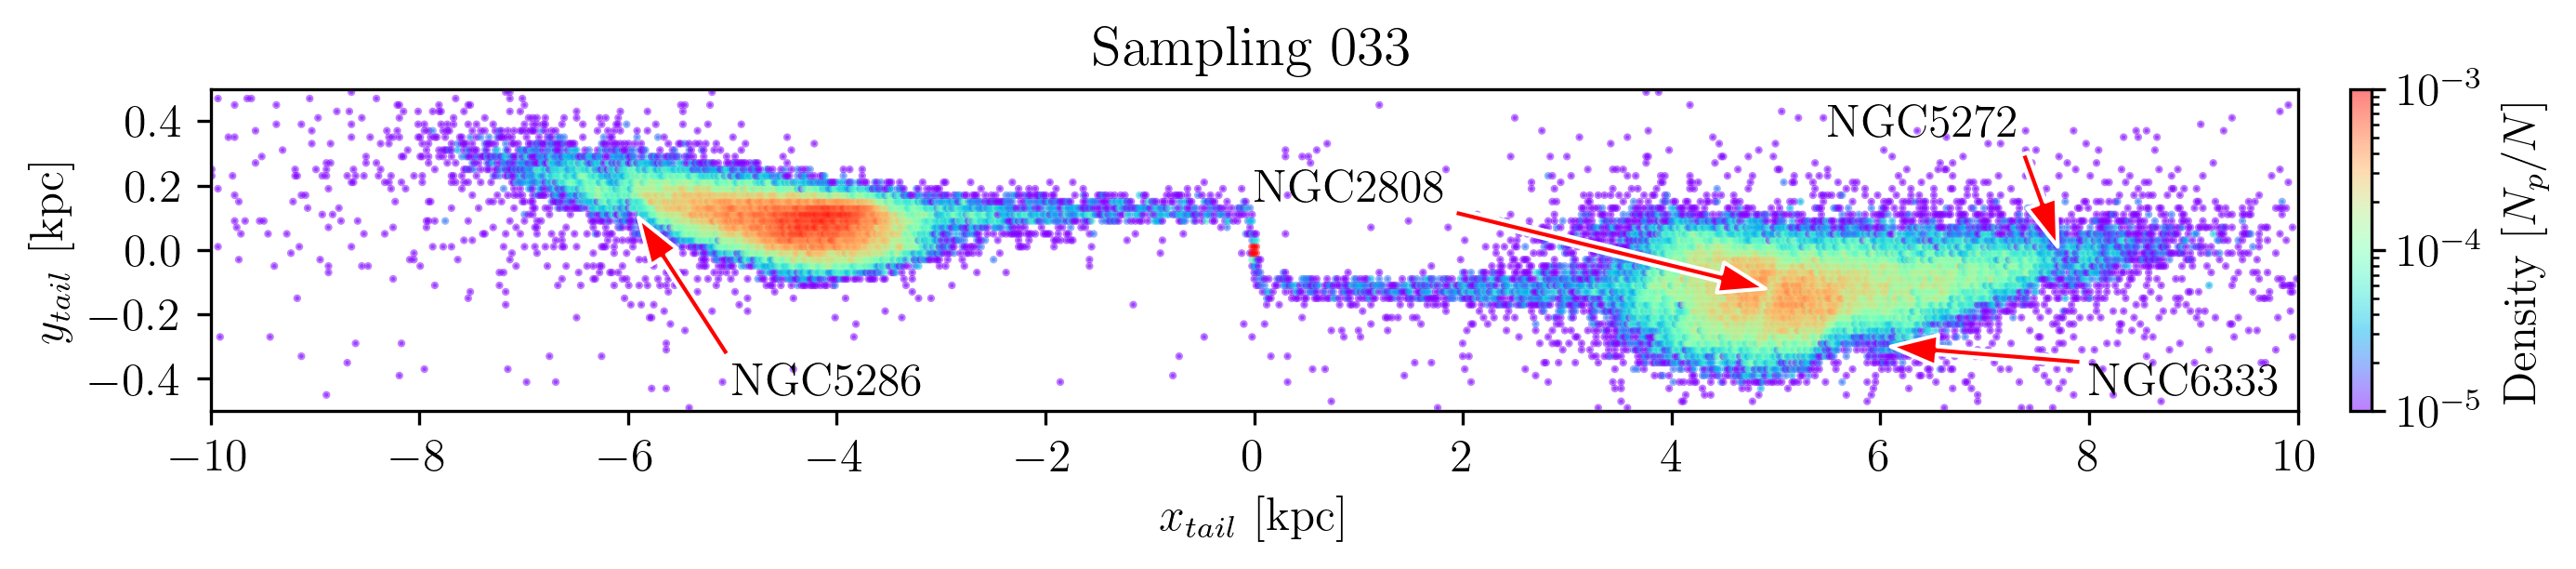
\includegraphics[width=\linewidth]{gallery_of_gaps_monte-carlo-033.png}
      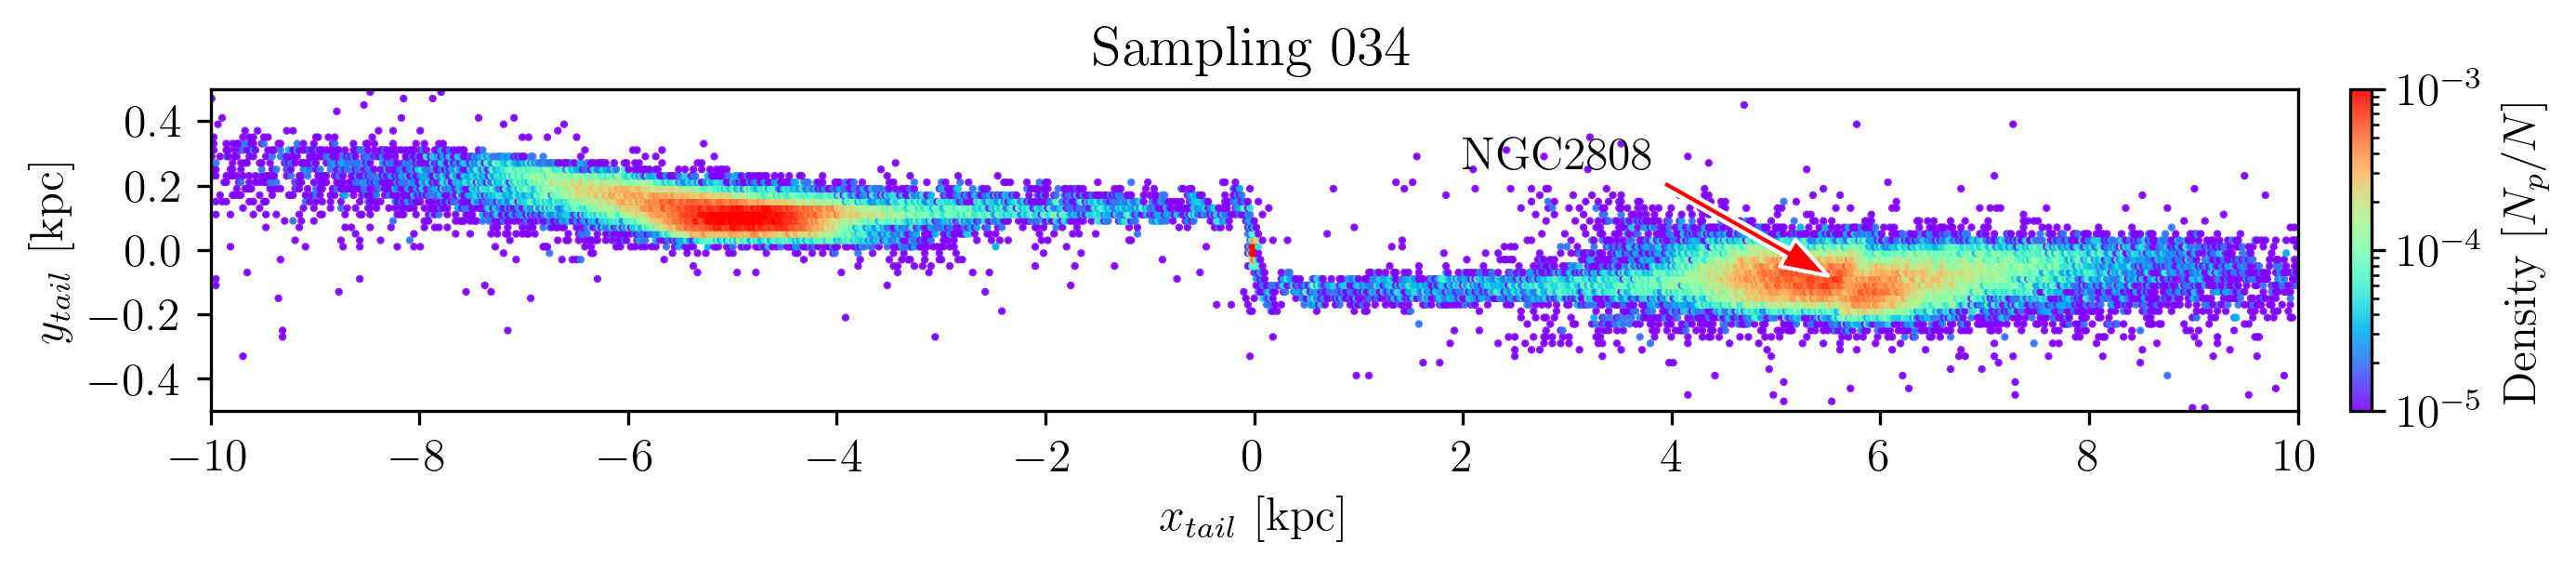
\includegraphics[width=\linewidth]{gallery_of_gaps_monte-carlo-034.png}      
      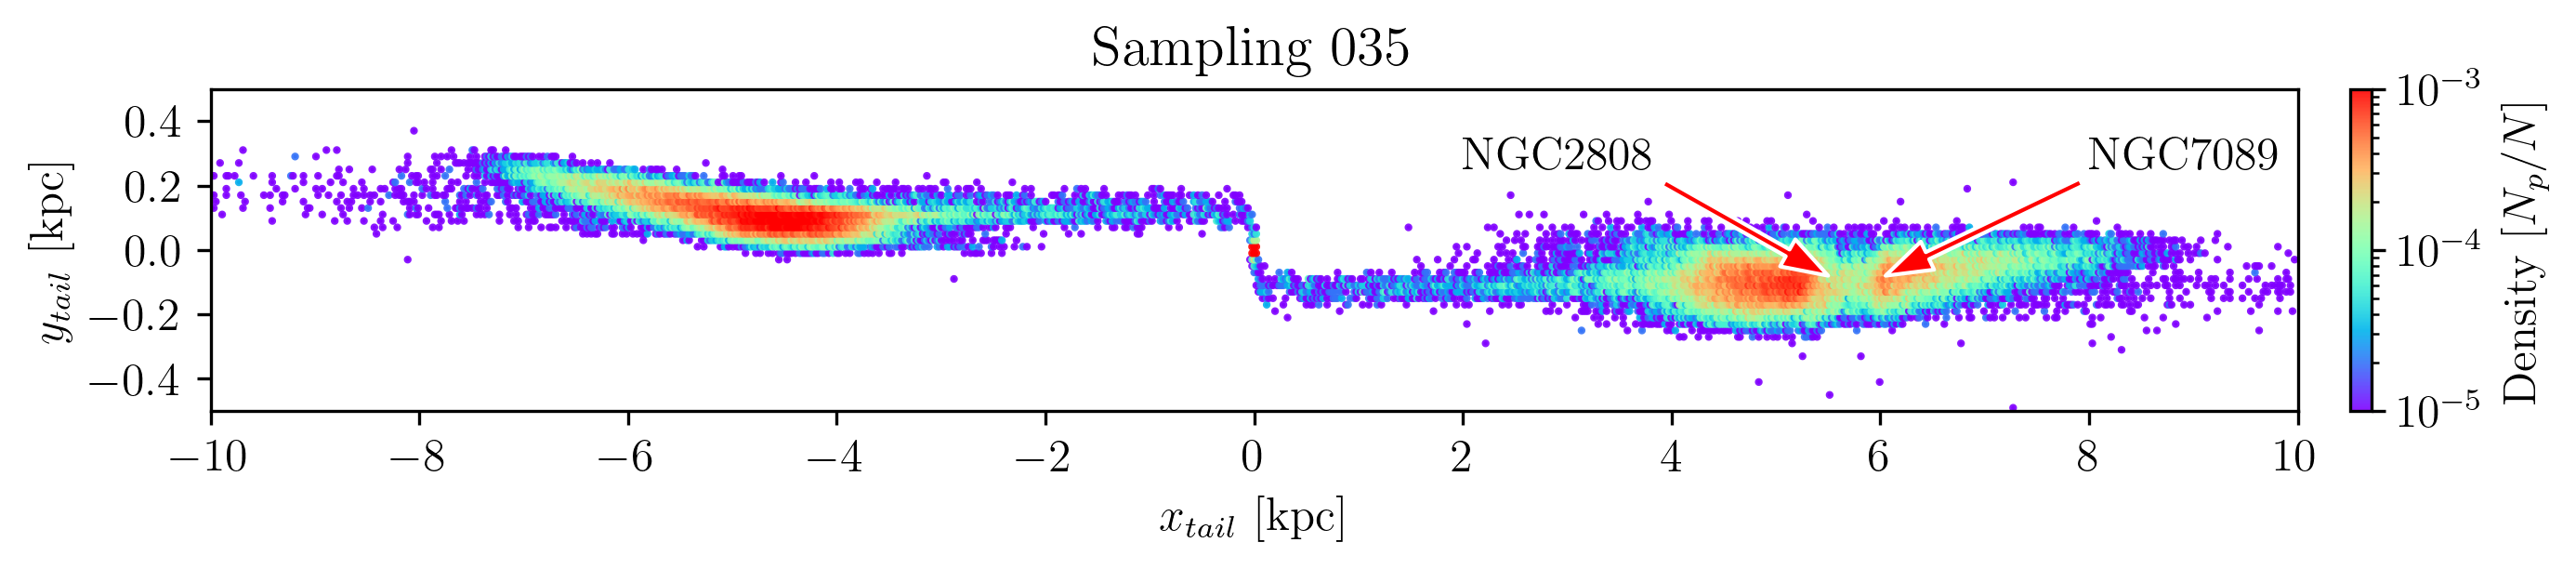
\includegraphics[width=\linewidth]{gallery_of_gaps_monte-carlo-035.png}
      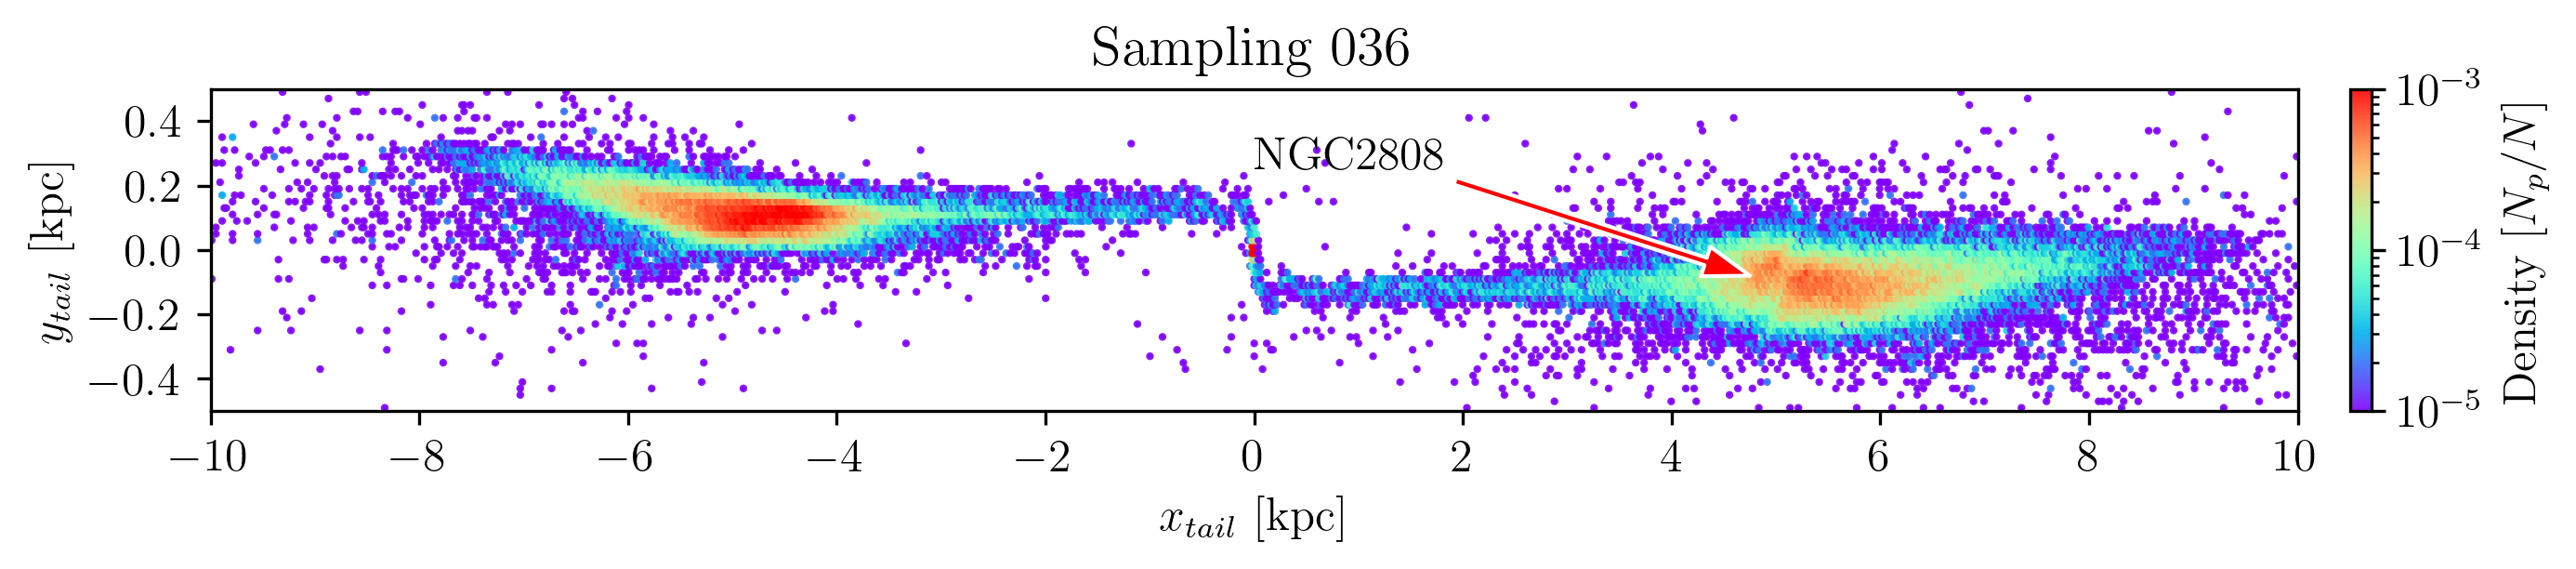
\includegraphics[width=\linewidth]{gallery_of_gaps_monte-carlo-036.png}      
      \caption{Ninth gap gallery}
      \label{fig:gallery8}
      \end{figure*}

    \begin{figure*}
      \centering
      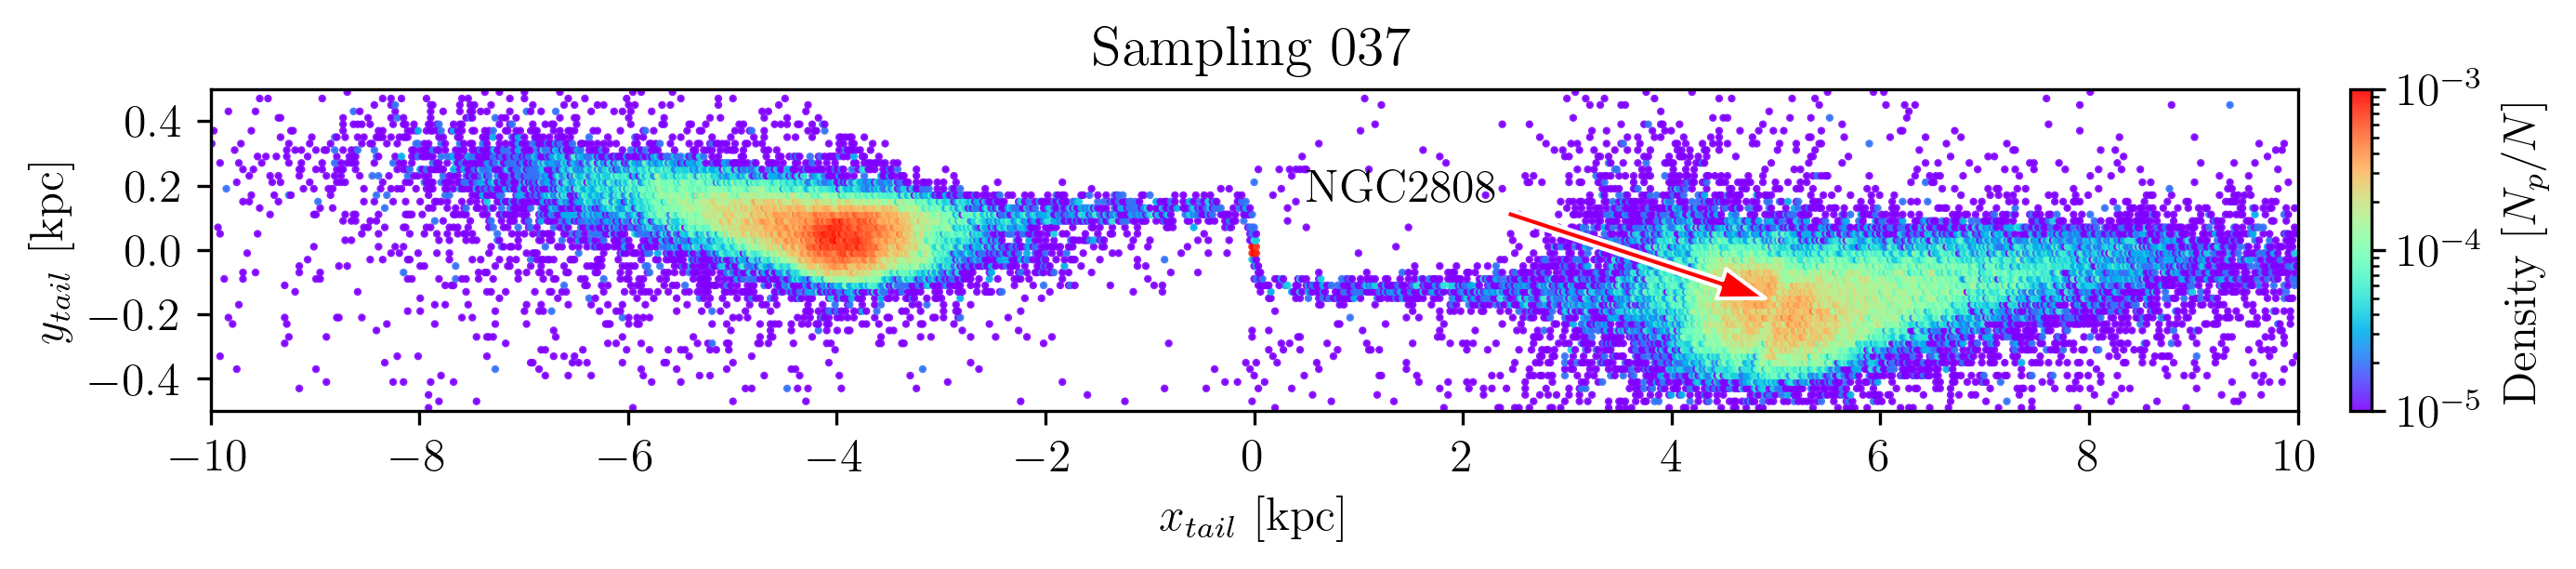
\includegraphics[width=\linewidth]{gallery_of_gaps_monte-carlo-037.png}
      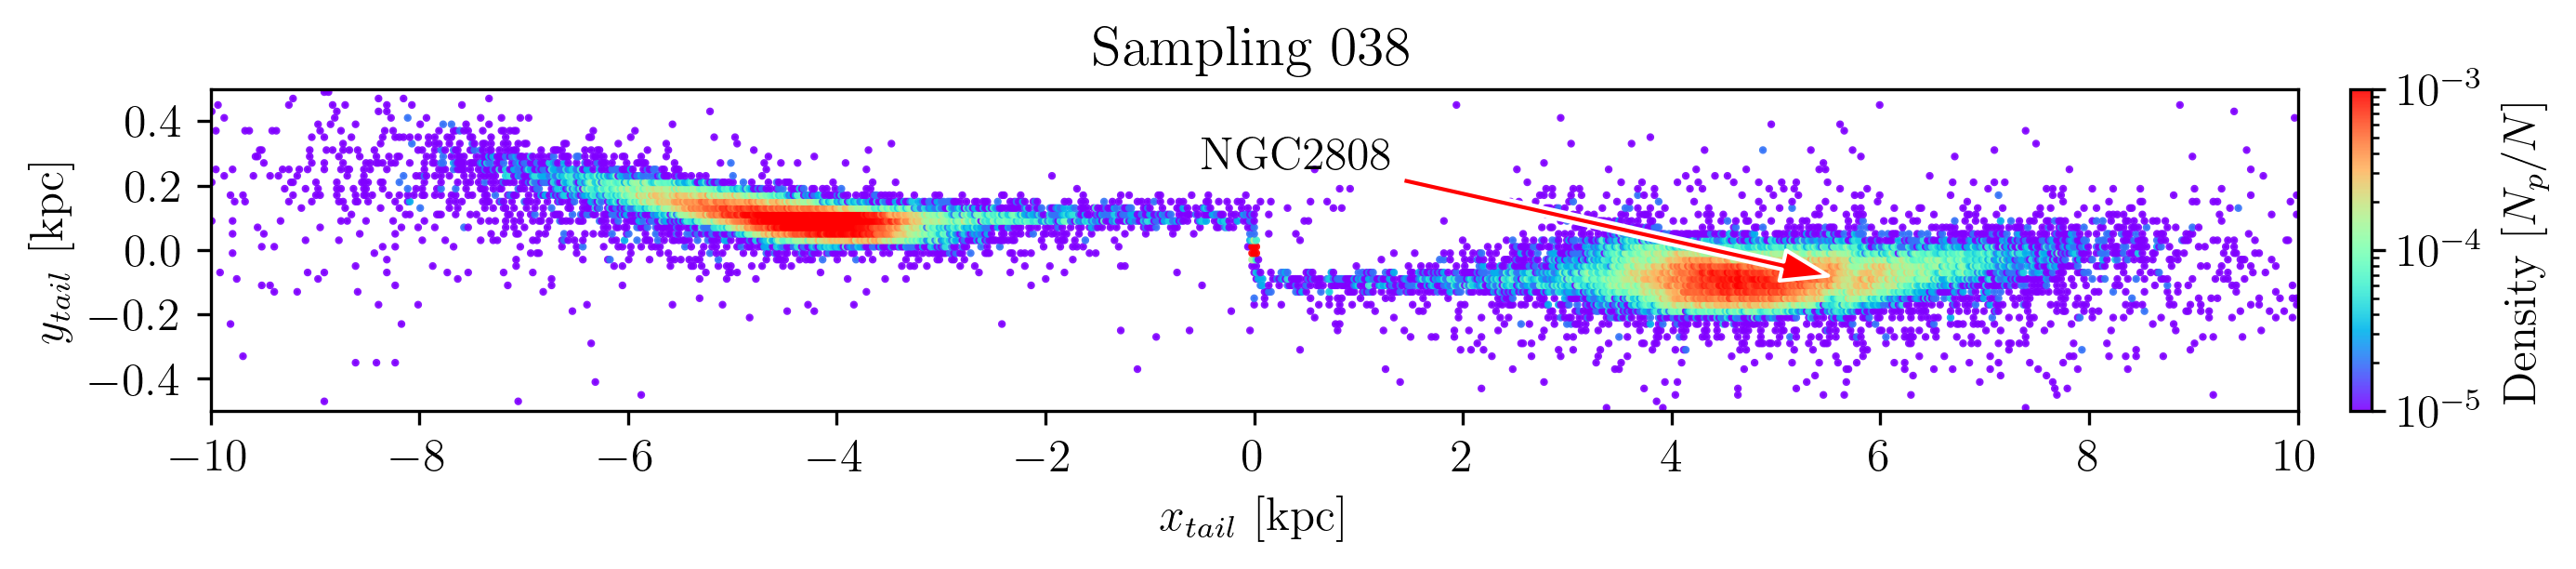
\includegraphics[width=\linewidth]{gallery_of_gaps_monte-carlo-038.png}
      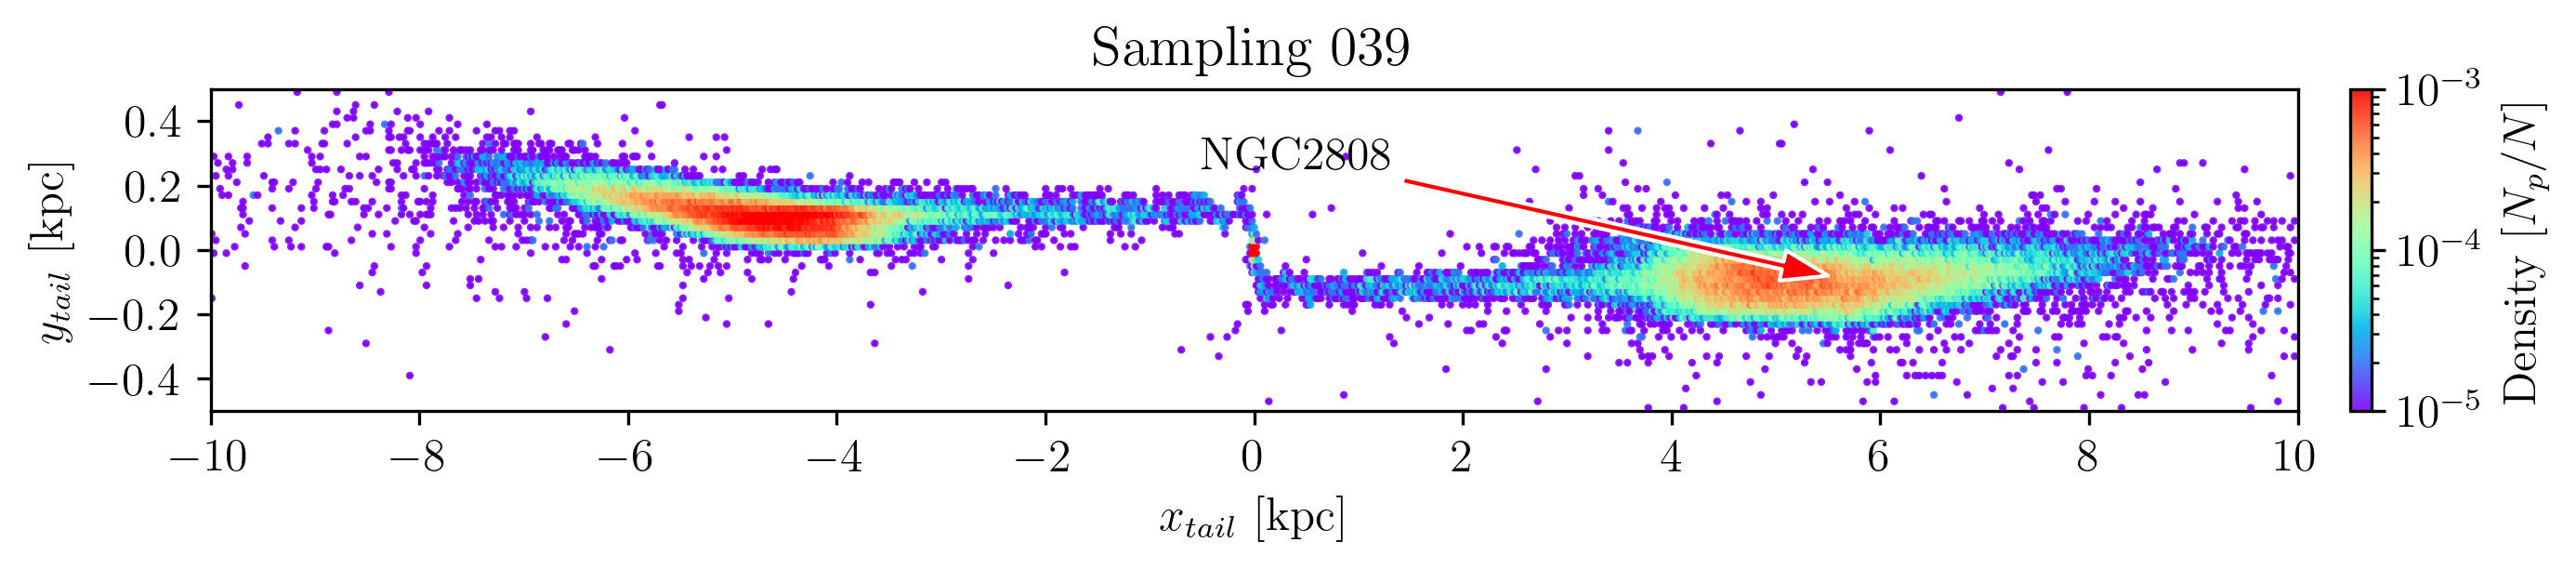
\includegraphics[width=\linewidth]{gallery_of_gaps_monte-carlo-039.png}
      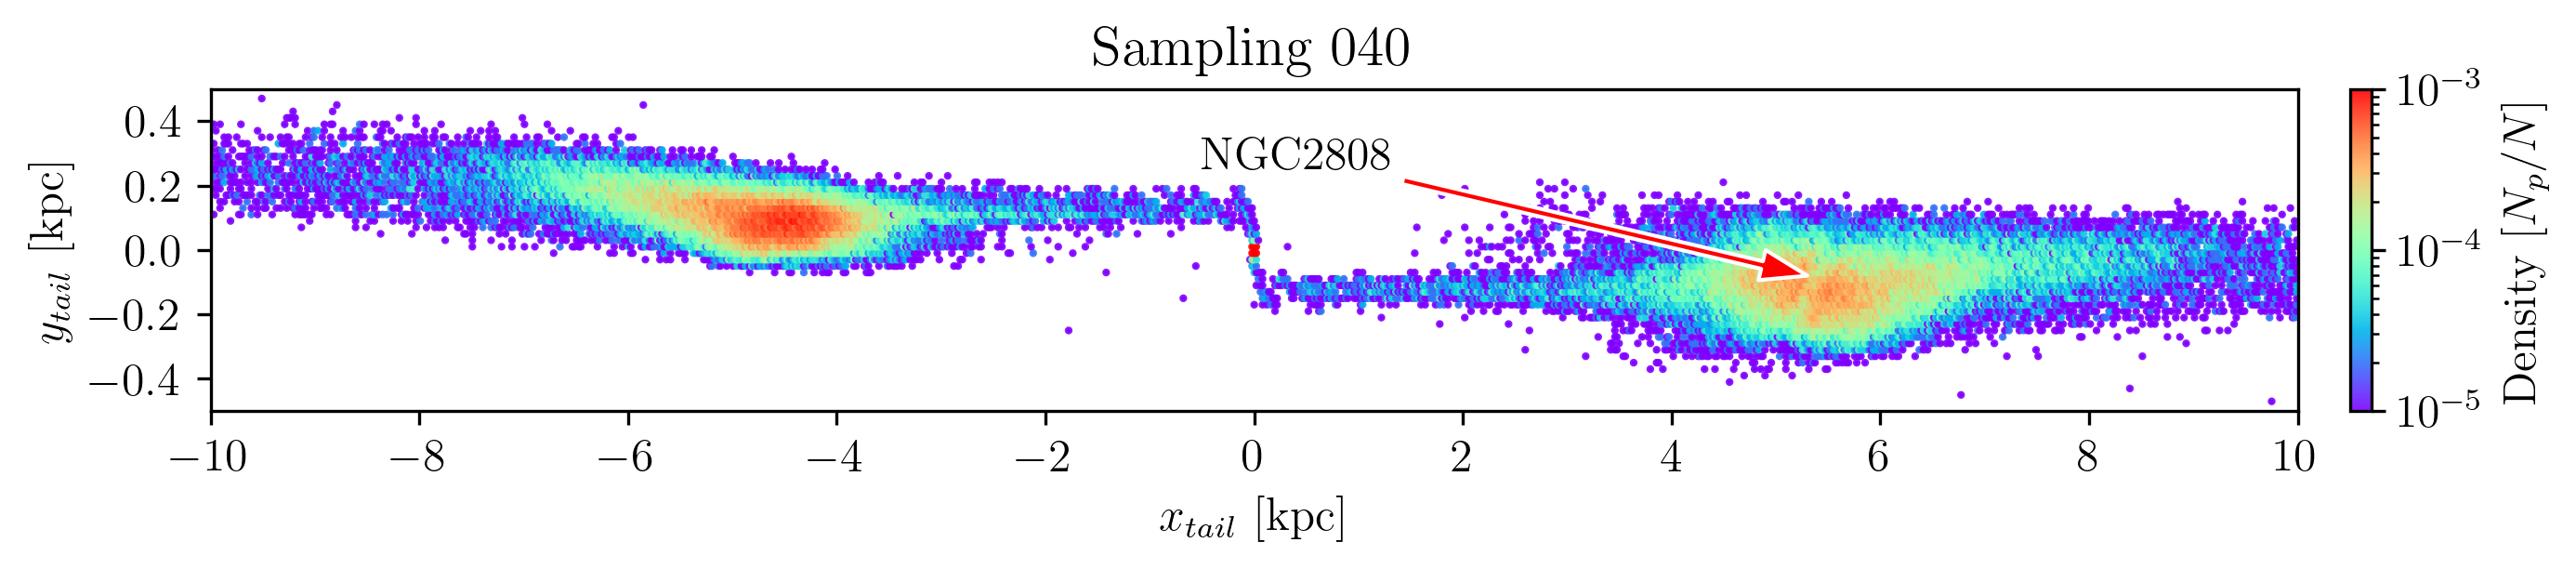
\includegraphics[width=\linewidth]{gallery_of_gaps_monte-carlo-040.png}
      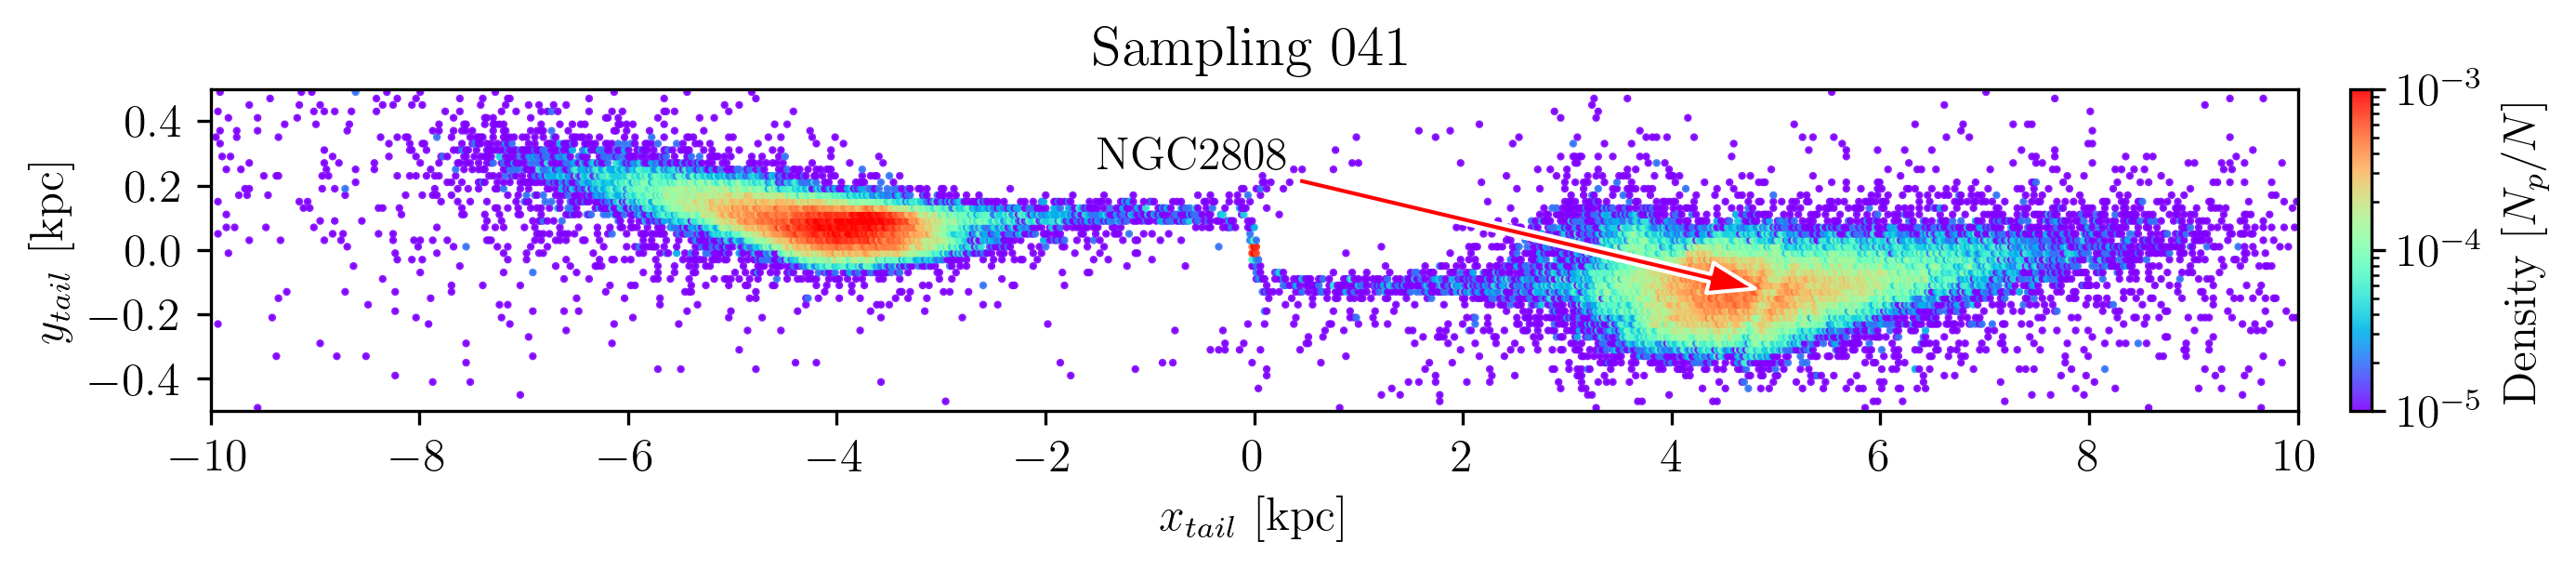
\includegraphics[width=\linewidth]{gallery_of_gaps_monte-carlo-041.png}      
      \caption{Tenth gap gallery}
      \label{fig:gallery9}
    \end{figure*}
    
    \begin{figure*}
      \centering
      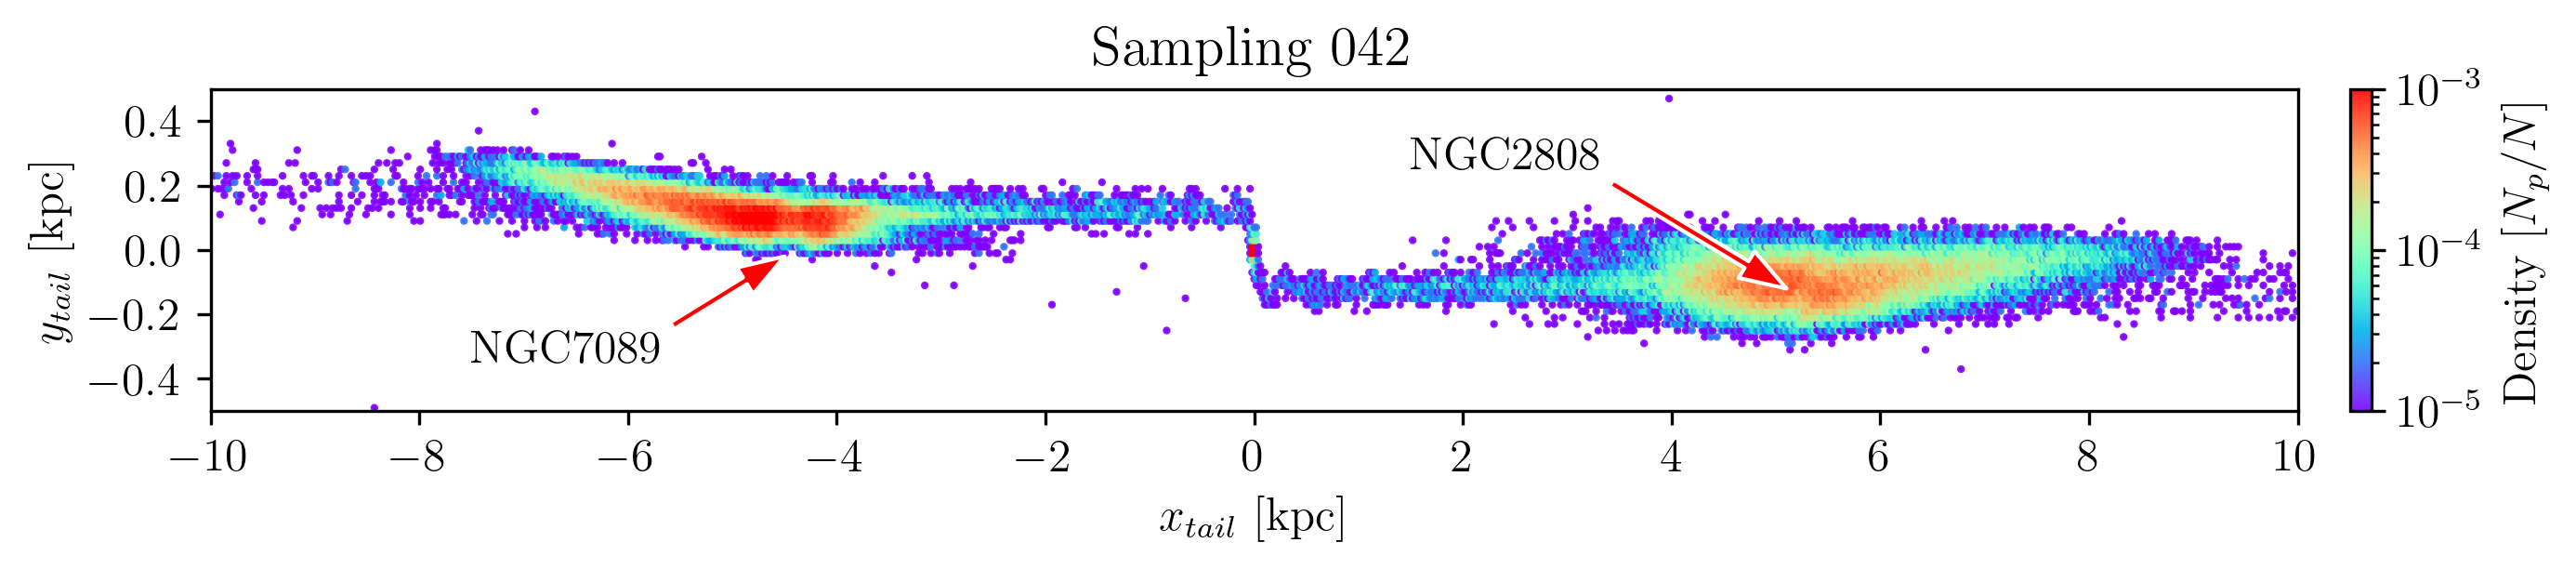
\includegraphics[width=\linewidth]{gallery_of_gaps_monte-carlo-042.png}
      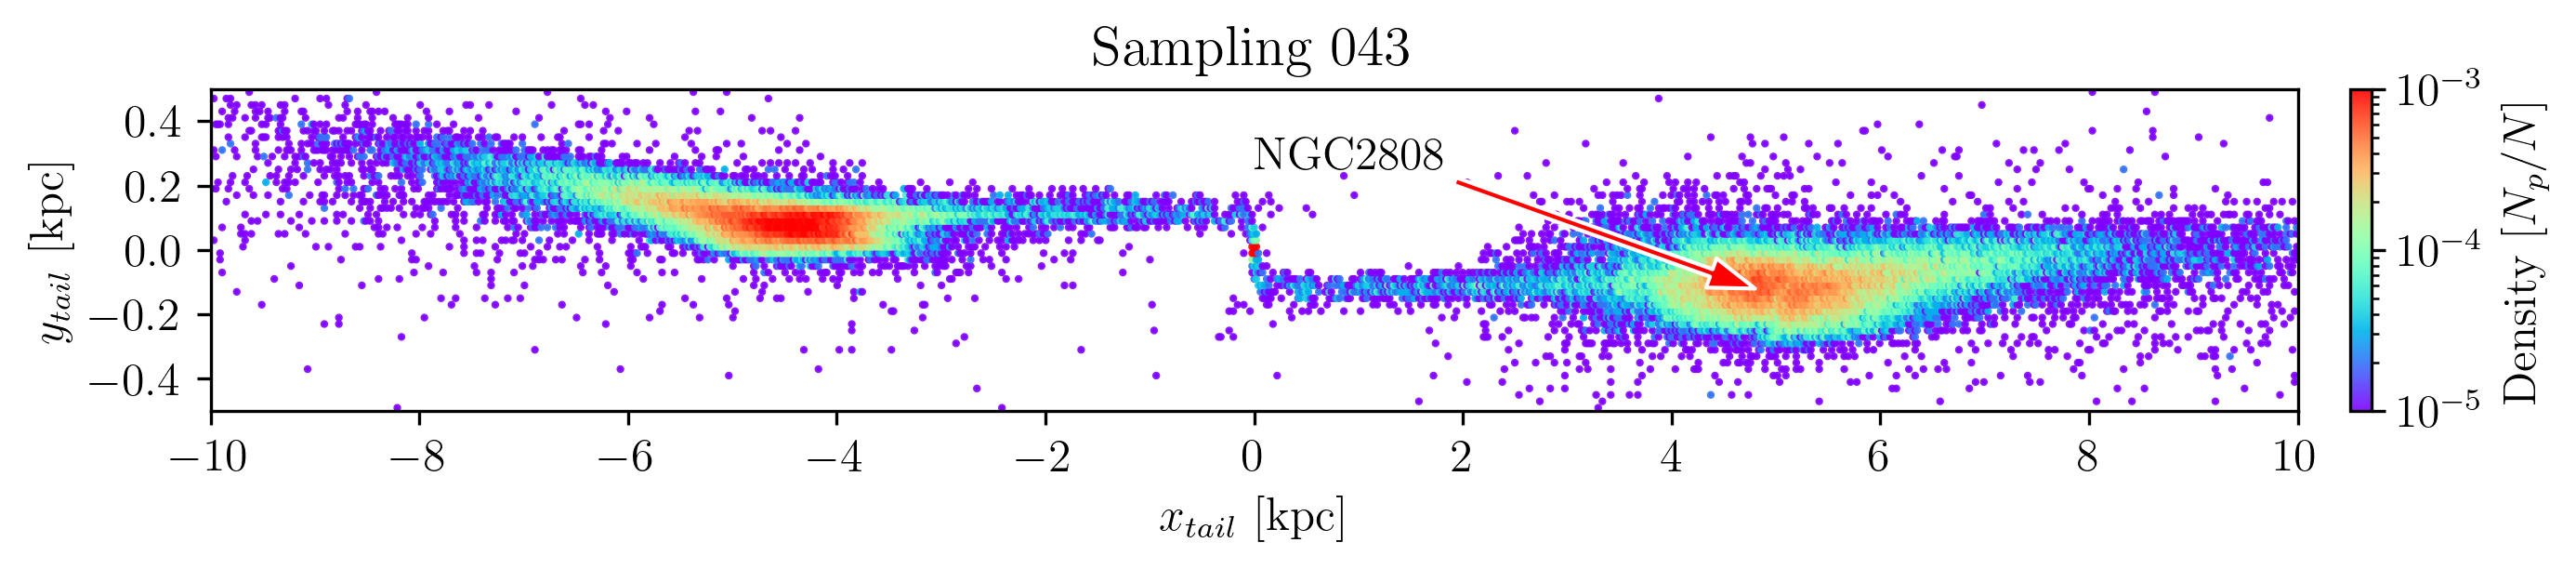
\includegraphics[width=\linewidth]{gallery_of_gaps_monte-carlo-043.png}
      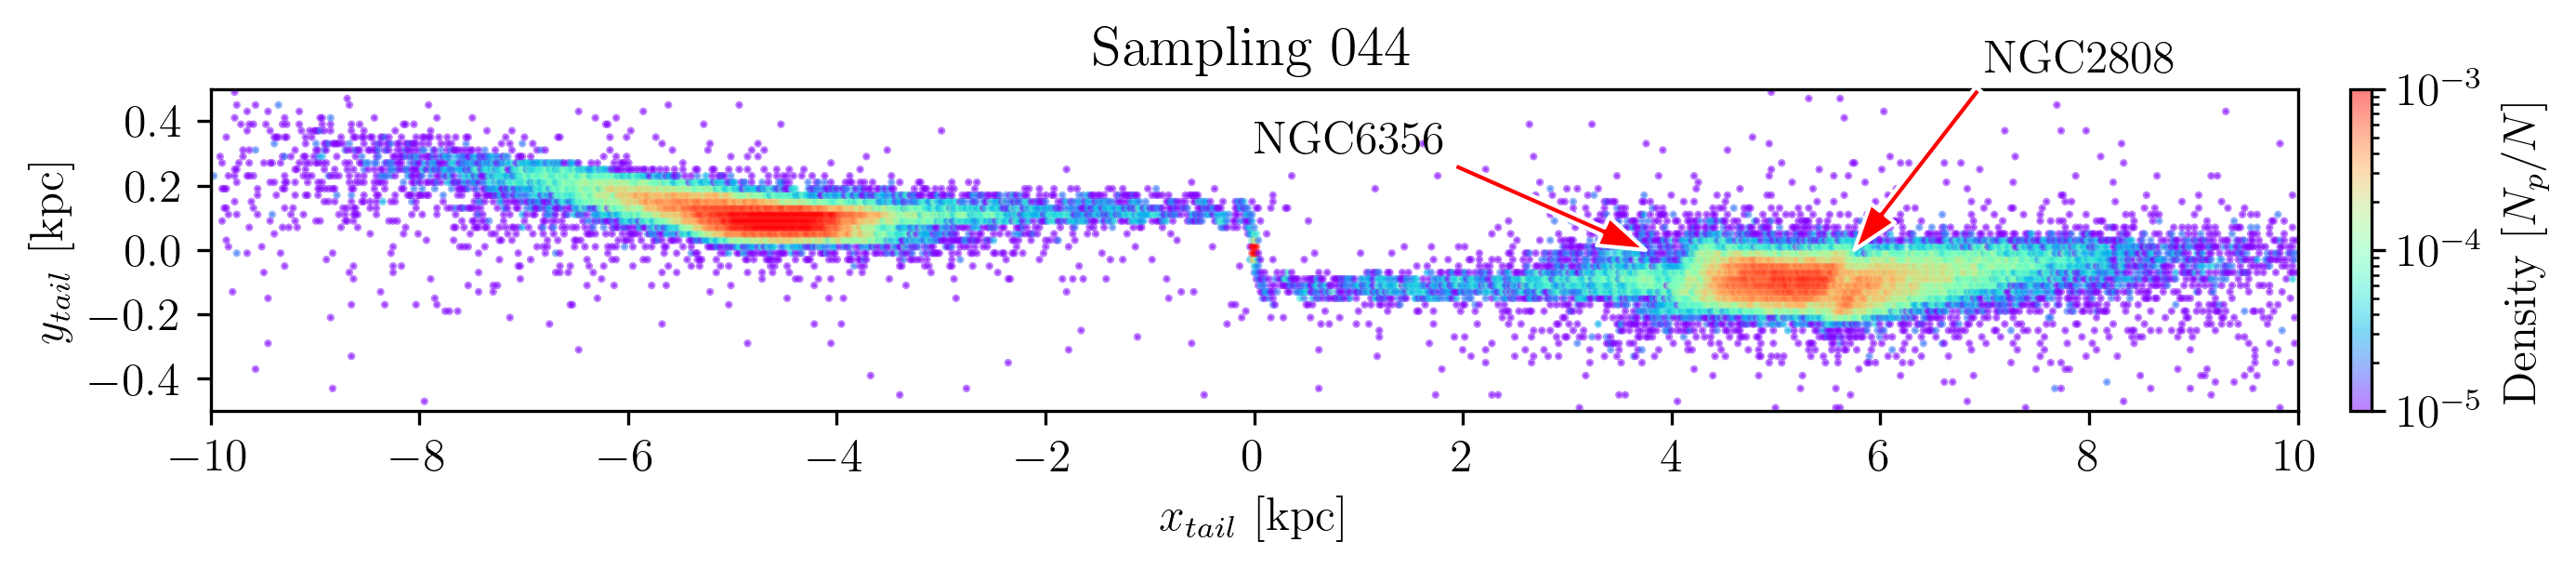
\includegraphics[width=\linewidth]{gallery_of_gaps_monte-carlo-044.png}
      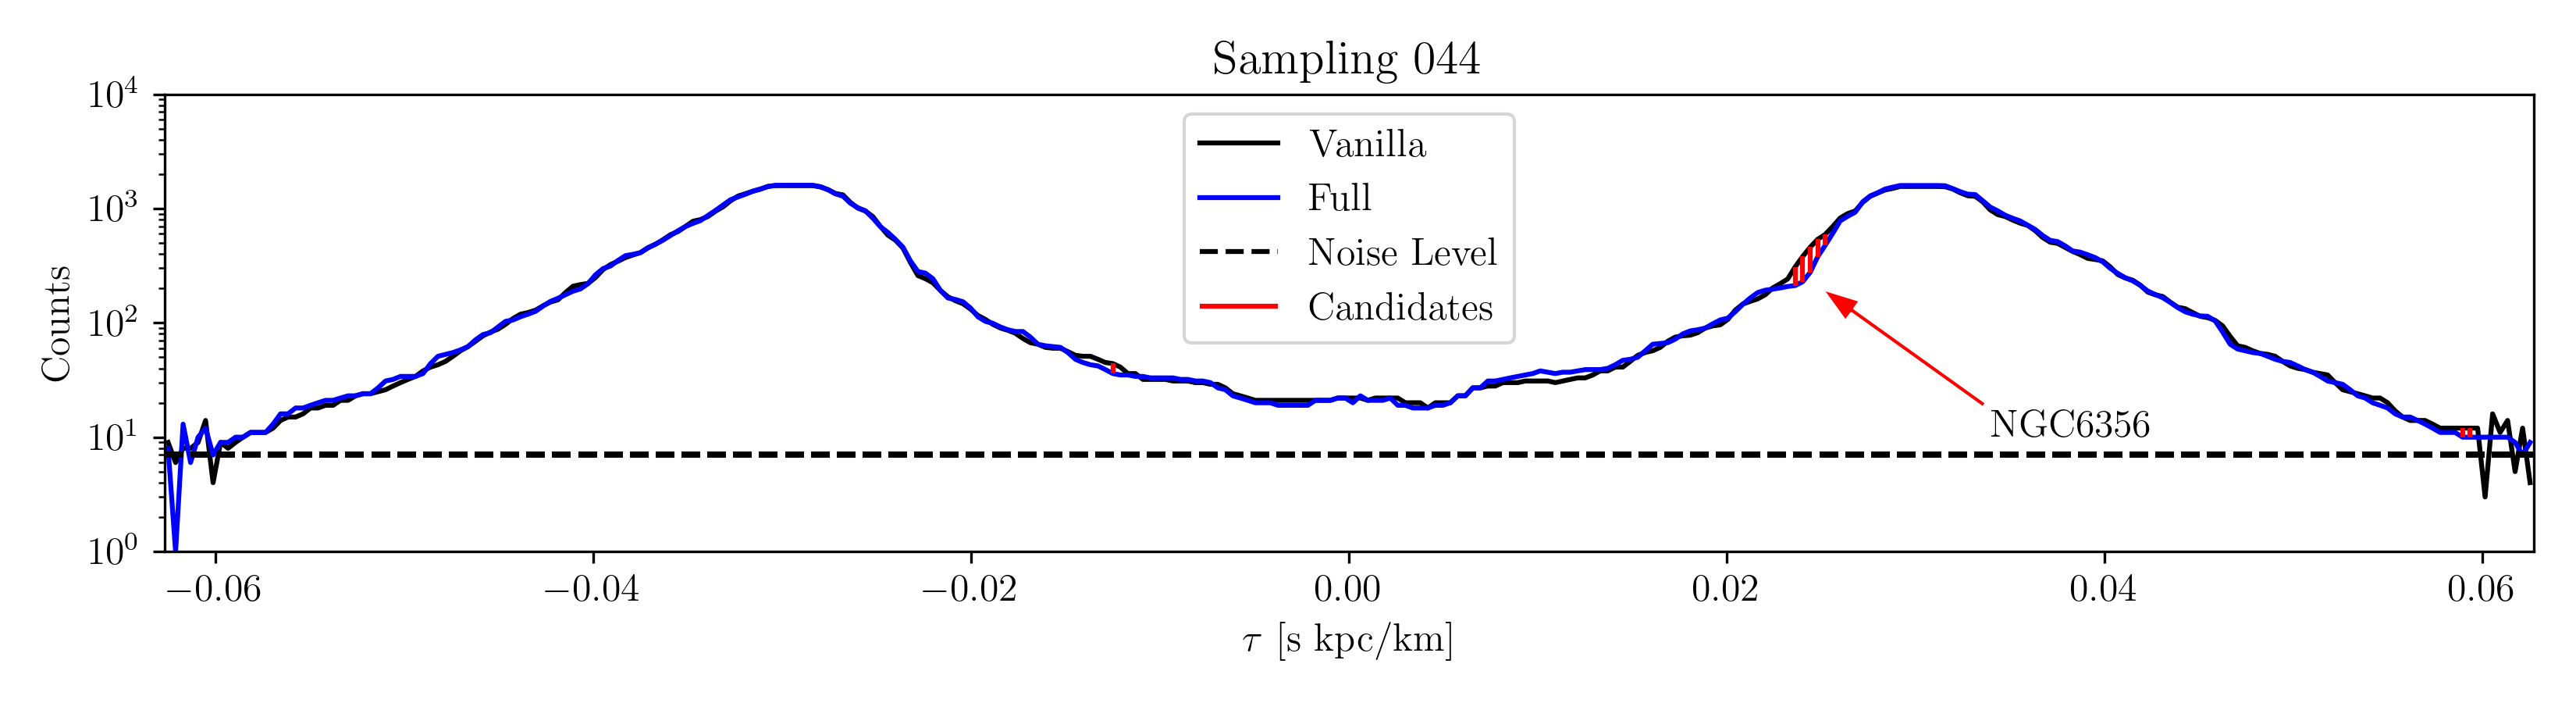
\includegraphics[width=\linewidth]{tau-profile-monte-carlo-044.png}
      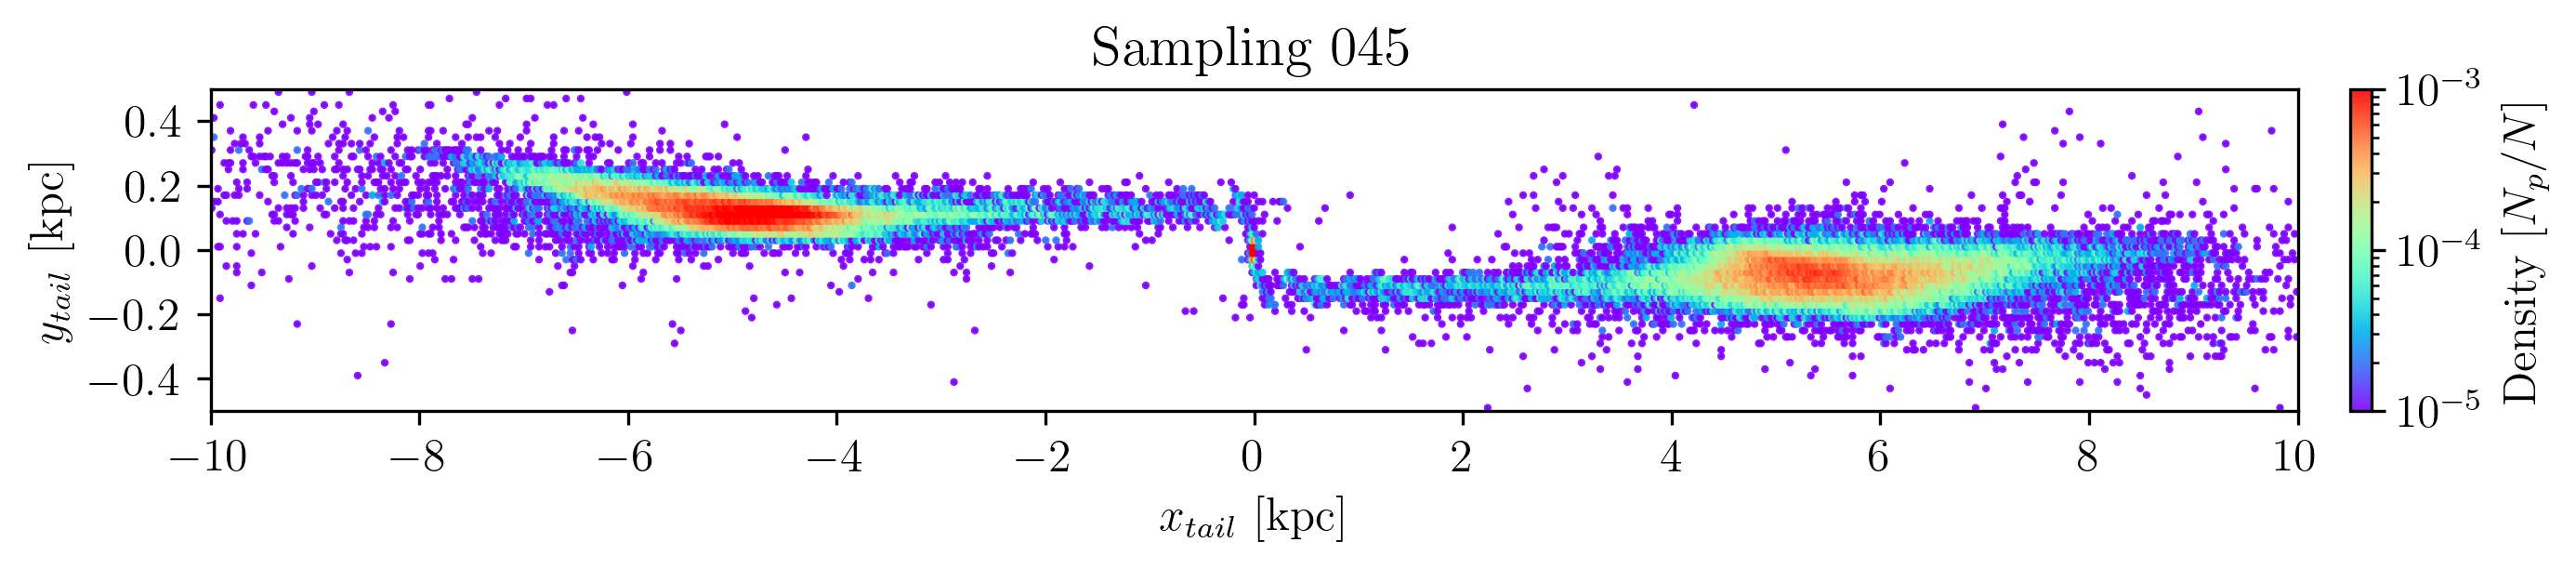
\includegraphics[width=\linewidth]{gallery_of_gaps_monte-carlo-045.png}
      \caption{Eleventh gap gallery}
      \label{fig:gallery010}
    \end{figure*}

    \begin{figure*}
      \centering
      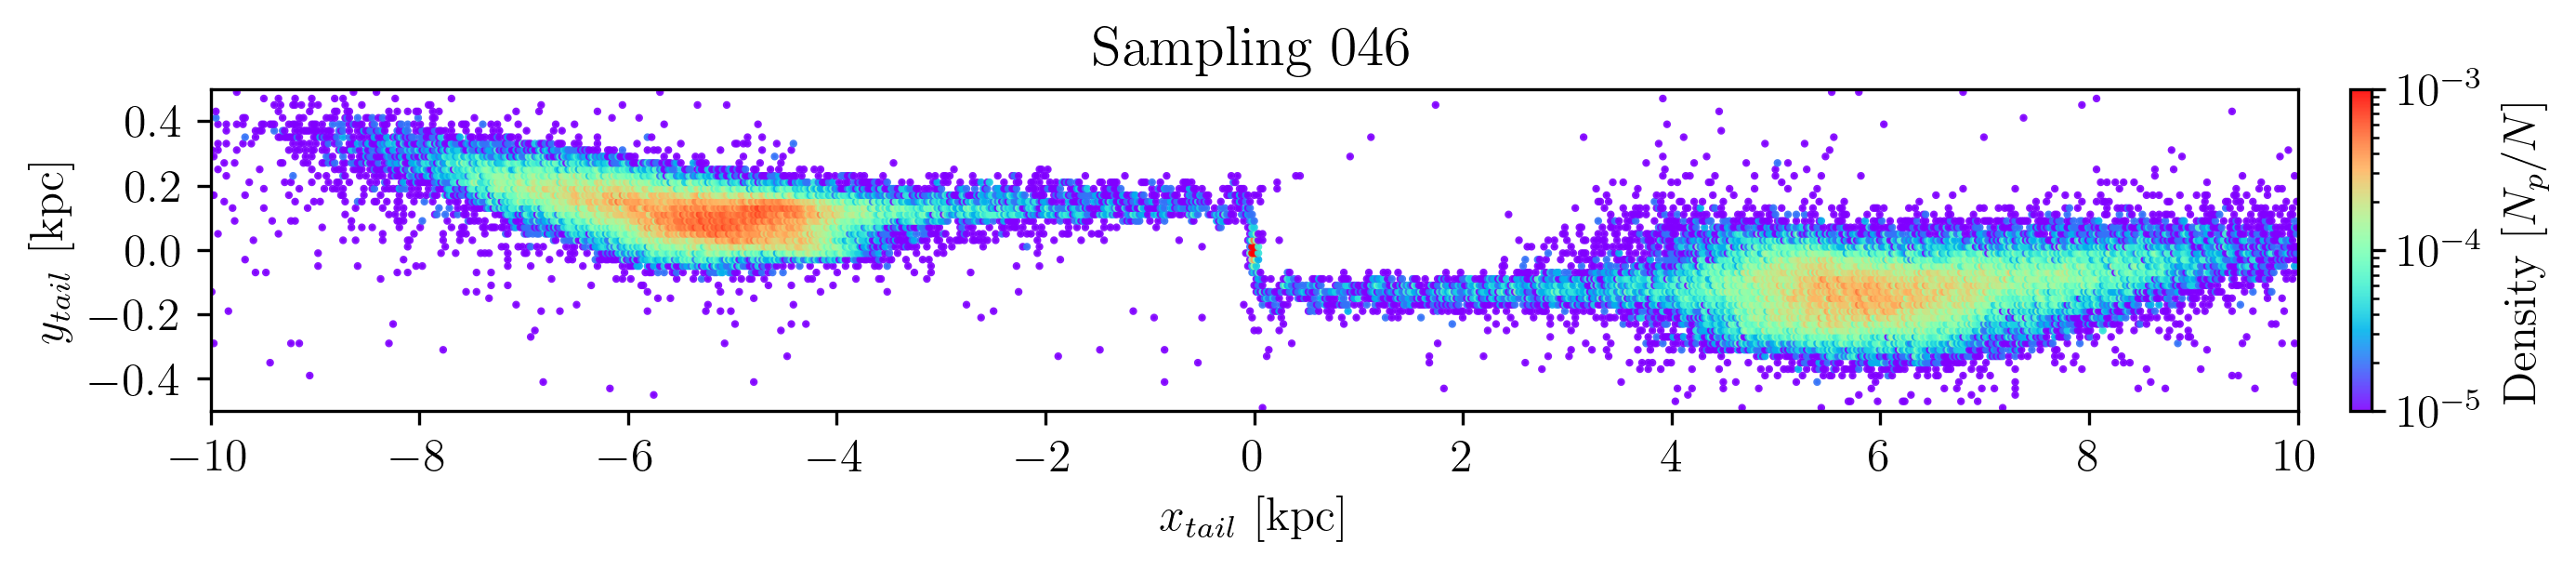
\includegraphics[width=\linewidth]{gallery_of_gaps_monte-carlo-046.png}
      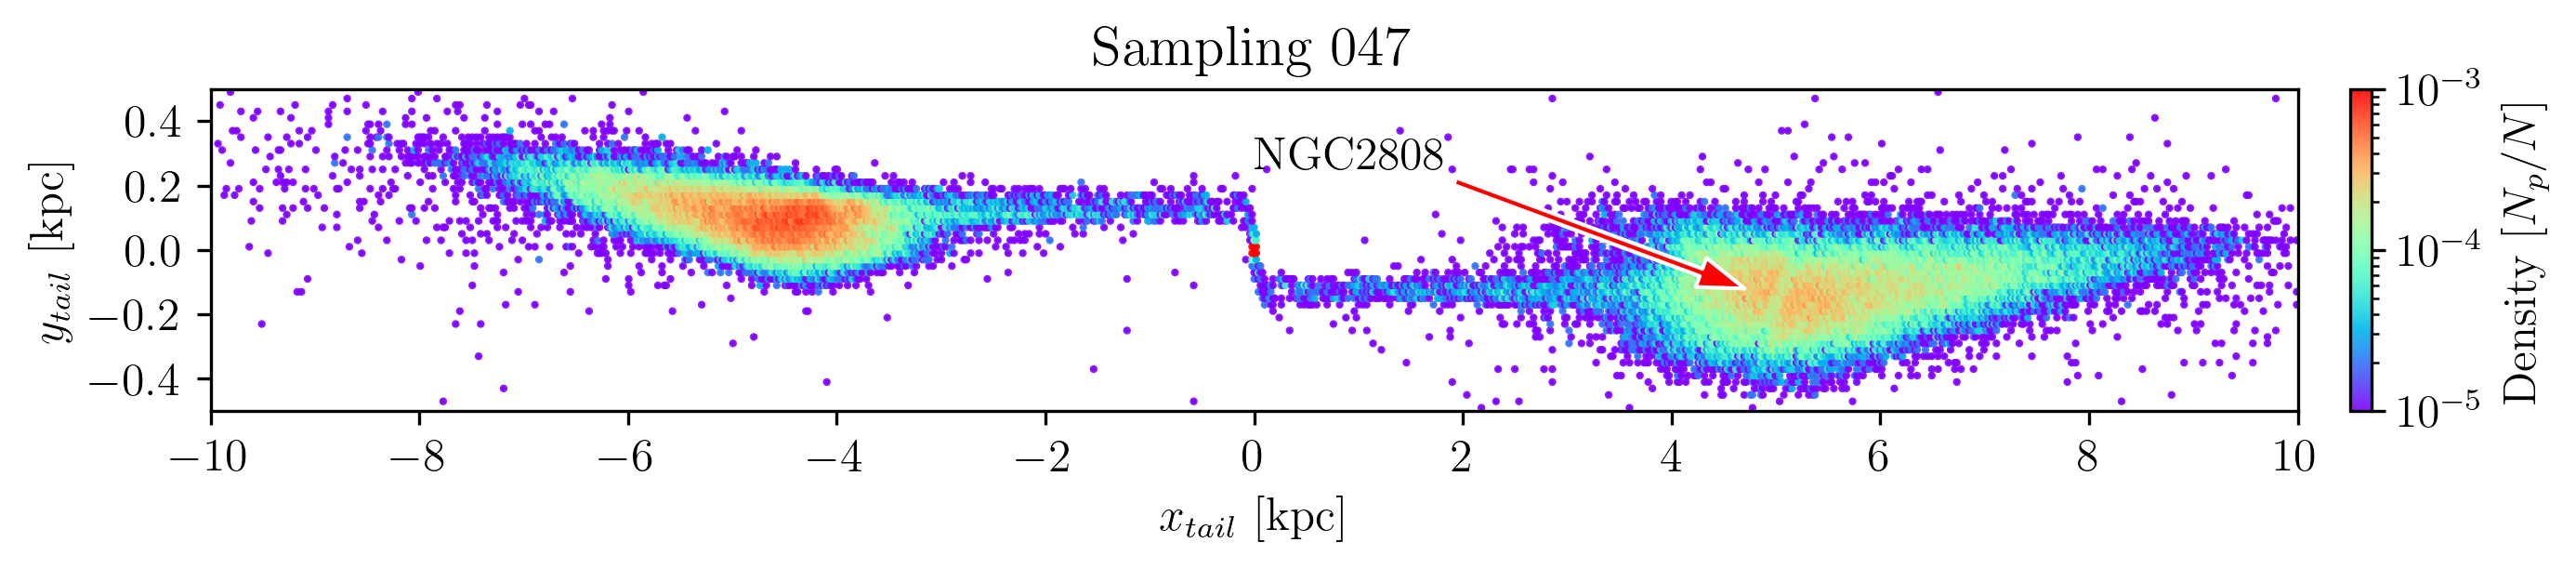
\includegraphics[width=\linewidth]{gallery_of_gaps_monte-carlo-047.png}
      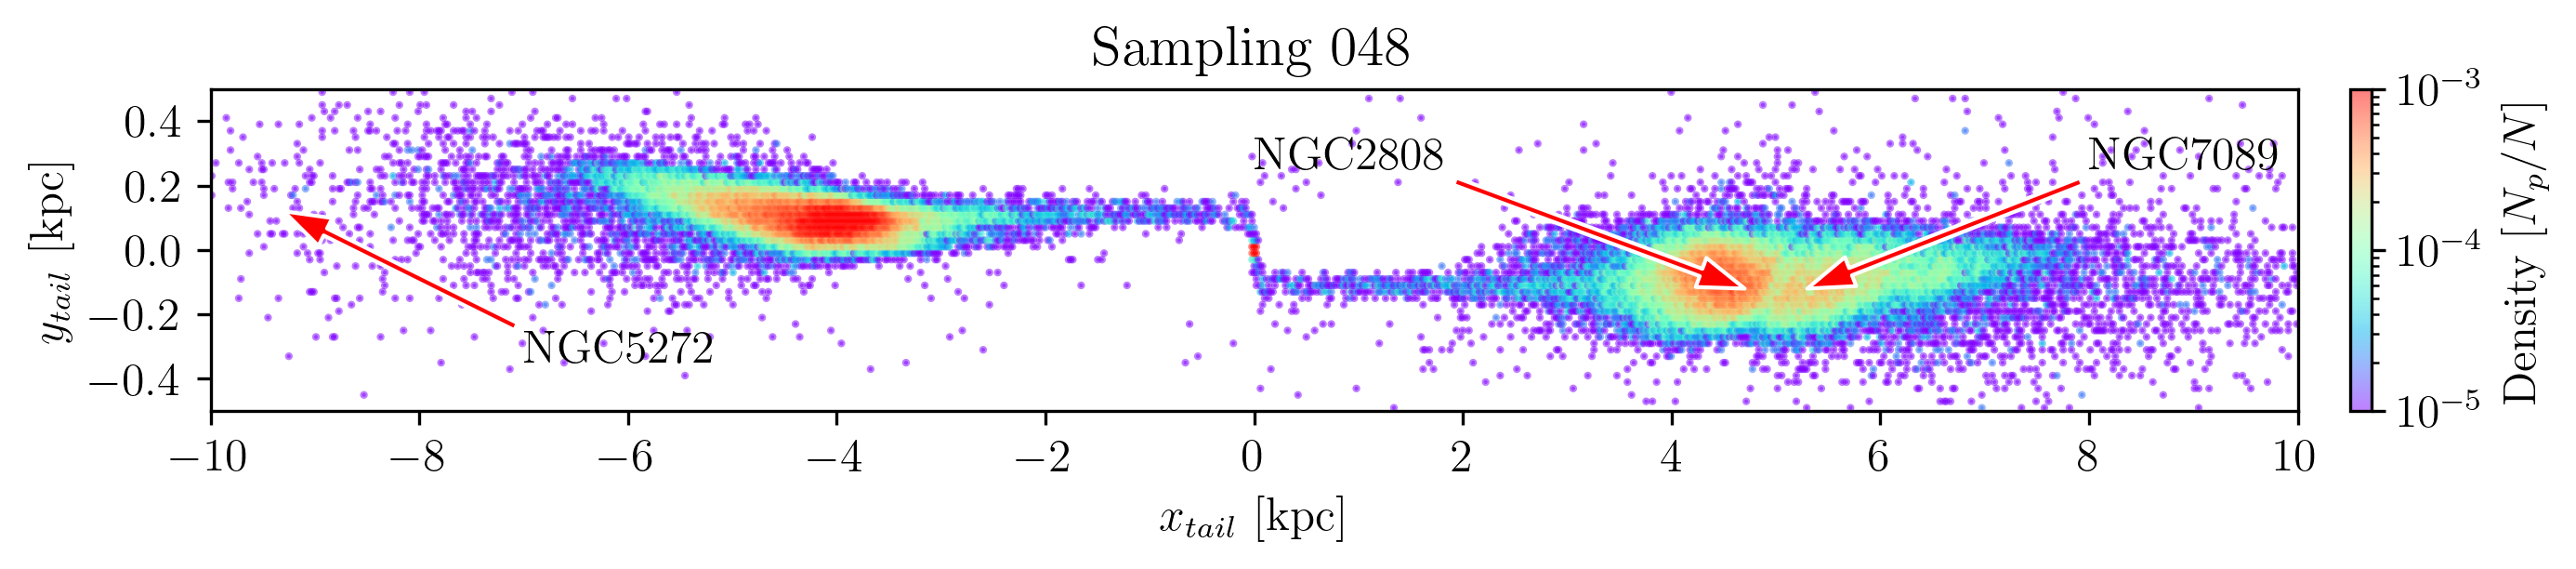
\includegraphics[width=\linewidth]{gallery_of_gaps_monte-carlo-048.png}
      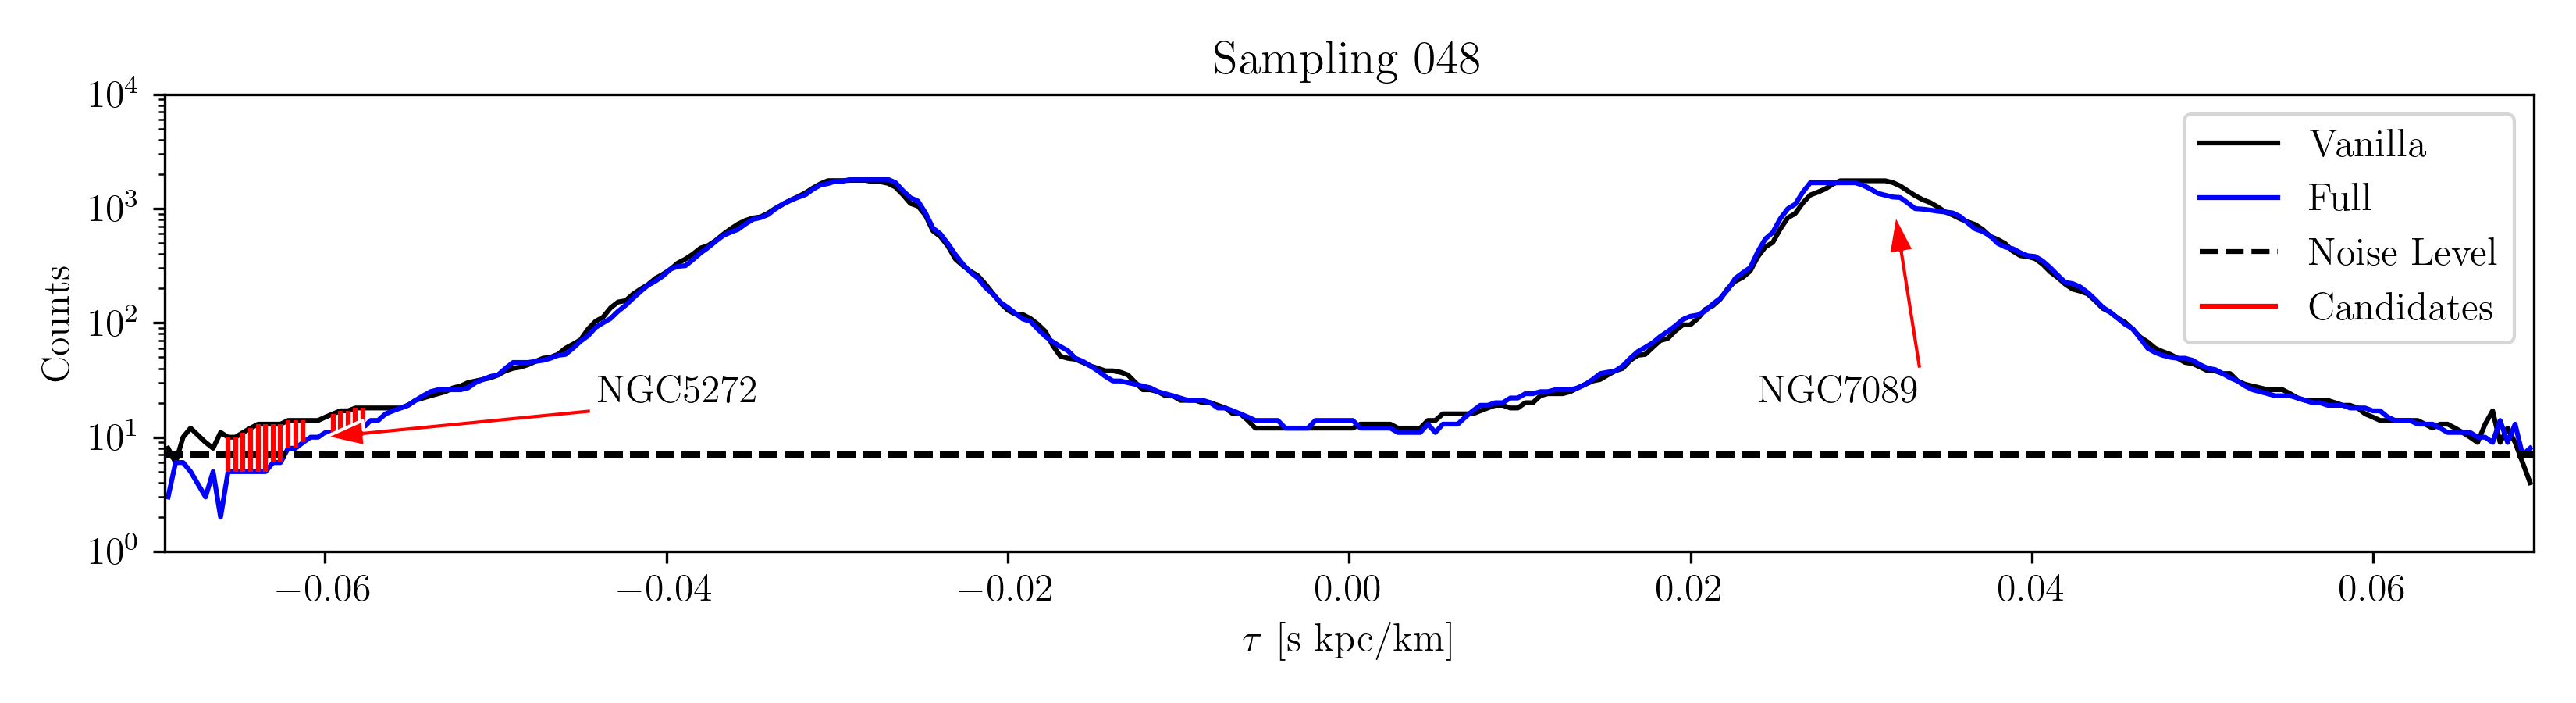
\includegraphics[width=\linewidth]{tau-profile-monte-carlo-048.png}
      
\includegraphics[width=\linewidth]{gallery_of_gaps_monte-carlo-049.png}
      \caption{Twelfth gap gallery}
      \label{fig:gallery11}
    \end{figure*}

\end{document}